%%%%%%%%%%%%%%%%%%%%%%%%%%%%%%%%%%%%%%%%%
% Masters Thesis 
% LaTeX Template
% Version 2.5 (27/8/17)
%
% This template was downloaded from:
% http://www.LaTeXTemplates.com
%
% Version 2.x major modifications by:
% Vel (vel@latextemplates.com)
%
% This template is based on a template by:
% Steve Gunn (http://users.ecs.soton.ac.uk/srg/softwaretools/document/templates/)
% Sunil Patel (http://www.sunilpatel.co.uk/thesis-template/)
%
% Template license:
% CC BY-NC-SA 3.0 (http://creativecommons.org/licenses/by-nc-sa/3.0/)
%
%%%%%%%%%%%%%%%%%%%%%%%%%%%%%%%%%%%%%%%%%

%----------------------------------------------------------------------------------------
%	PACKAGES AND OTHER DOCUMENT CONFIGURATIONS
%----------------------------------------------------------------------------------------

\documentclass[
12pt, % The default document font size, options: 10pt, 11pt, 12pt
oneside, % Two side (alternating margins) for binding by default, uncomment to switch to one side
english, % ngerman for German
draft=false,
doublespacing, % Single line spacing, alternatives: onehalfspacing or doublespacing
%nolistspacing, % If the document is onehalfspacing or doublespacing, uncomment this to set spacing in lists to single
liststotoc, % Uncomment to add the list of figures/tables/etc to the table of contents
toctotoc, % Uncomment to add the main table of contents to the table of contents
parskip, % Uncomment to add space between paragraphs
%nohyperref, % Uncomment to not load the hyperref package
headsepline, % Uncomment to get a line under the header
%chapterinoneline, % Uncomment to place the chapter title next to the number on one line
%consistentlayout, % Uncomment to change the layout of the declaration, abstract and acknowledgements pages to match the default layout
]{MastersDoctoralThesis} % The class file specifying the document structure

\usepackage[utf8]{inputenc} % Required for inputting international characters
\usepackage[T1]{fontenc} % Output font encoding for international characters

\usepackage{mathpazo} % Use the Palatino font by default
\usepackage{graphicx}

\usepackage[backend=bibtex,natbib=true]{biblatex} % Use the bibtex backend

\addbibresource{bibliography.bib} % The filename of the bibliography

\usepackage[autostyle=true]{csquotes} % Required to generate language-dependent quotes in the bibliography

\usepackage[ruled, linesnumbered,noend]{algorithm2e} % For algorithms

% for function graphs
\usepackage{tikz}
\usepackage{color}
\usetikzlibrary{datavisualization}
\usetikzlibrary{datavisualization.formats.functions}

\usepackage{hhline}
\usepackage{rotating}
\usepackage{multirow}
\usepackage{longtable}
\usepackage{lscape}
\usepackage{adjustbox}
\usepackage{array}
\usepackage{booktabs}

\newcolumntype{R}[2]{%
    >{\adjustbox{angle=#1,lap=\width-(#2)}\bgroup}%
    l%
    <{\egroup}%
}
\newcommand*\rot{\multicolumn{1}{R{90}{1em}}}

\usepackage{dingbat}

\newcommand{\blueline}{\raisebox{2pt}{\tikz{\draw[-,black!40!blue,solid,line width = 0.9pt](0,0) -- (5mm,0);}}}
\newcommand{\yellowline}{\raisebox{2pt}{\tikz{\draw[-,black!40!yellow,solid,line width = 0.9pt](0,0) -- (5mm,0);}}}
\newcommand{\redline}{\raisebox{2pt}{\tikz{\draw[-,black!40!red,solid,line width = 0.9pt](0,0) -- (5mm,0);}}}

% for math conditions
\usepackage{amsmath}

\SetKwProg{Fn}{function}{}{}

%----------------------------------------------------------------------------------------
%	MARGIN SETTINGS
%----------------------------------------------------------------------------------------

\geometry{
	paper=letterpaper, % Change to letterpaper for US letter
	inner=2.5cm, % Inner margin
	outer=3.8cm, % Outer margin
	bindingoffset=.5cm, % Binding offset
	top=1.5cm, % Top margin
	bottom=1.5cm, % Bottom margin
	%showframe, % Uncomment to show how the type block is set on the page
}

%----------------------------------------------------------------------------------------
%	THESIS INFORMATION
%----------------------------------------------------------------------------------------

\thesistitle{Semi-Supervised Hybrid Windowing Ensembles for Learning from Evolving Streams} % Your thesis title, this is used in the title and abstract, print it elsewhere with \ttitle
\supervisor{Dr. Herna \textsc{Viktor}} % Your supervisor's name, this is used in the title page, print it elsewhere with \supname
\examiner{} % Your examiner's name, this is not currently used anywhere in the template, print it elsewhere with \examname
\degree{Master of Science in Computer Science} % Your degree name, this is used in the title page and abstract, print it elsewhere with \degreename
\author{Sean Louis Alan \textsc{Floyd}} % Your name, this is used in the title page and abstract, print it elsewhere with \authorname

\subject{Computer Science} % Your subject area, this is not currently used anywhere in the template, print it elsewhere with \subjectname
\keywords{} % Keywords for your thesis, this is not currently used anywhere in the template, print it elsewhere with \keywordnames
\university{\href{https://uottawa.ca}{University of Ottawa}} % Your university's name and URL, this is used in the title page and abstract, print it elsewhere with \univname
\department{\href{https://engineering.uottawa.ca}{School of Electrical Engineering and Computer Science\\ Faculty of Engineering}} % Your department's name and URL, this is used in the title page and abstract, print it elsewhere with \deptname
\group{\href{http://researchgroup.university.com}{Research Group Name}} % Your research group's name and URL, this is used in the title page, print it elsewhere with \groupname
\faculty{\href{http://faculty.university.com}{Faculty of Graduate and Postdoctoral Studies}} % Your faculty's name and URL, this is used in the title page and abstract, print it elsewhere with \facname

\AtBeginDocument{
\hypersetup{pdftitle=\ttitle} % Set the PDF's title to your title
\hypersetup{pdfauthor=\authorname} % Set the PDF's author to your name
\hypersetup{pdfkeywords=\keywordnames} % Set the PDF's keywords to your keywords
}

\begin{document}

\frontmatter % Use roman page numbering style (i, ii, iii, iv...) for the pre-content pages

%\pagestyle{plain} % Default to the plain heading style until the thesis style is called for the body content

%----------------------------------------------------------------------------------------
%	TITLE PAGE
%----------------------------------------------------------------------------------------

\begin{titlepage}
\begin{center}

\vspace*{.05\textheight}

\HRule \\[0.4cm] % Horizontal line
{\huge \bfseries \ttitle\par}\vspace{0.4cm} % Thesis title
\HRule \\[1.5cm] % Horizontal line
 
\large \authorname % Author name - remove the \href bracket to remove the link
 
\vfill

Thesis submitted in partial fulfilment of the requirements for the \\
\textbf{\degreename}\\[0.3cm] % University requirement text
\deptname\\\univname{}\\[2cm] % Research group name and department name
 
\vfill

{\copyright \authorname, Ottawa, Canada, 2019}\\[4cm] % Date
% \includegraphics{Logo} % University/department logo - uncomment to place it
\end{center}
\end{titlepage}

%----------------------------------------------------------------------------------------
%	ABSTRACT PAGE
%----------------------------------------------------------------------------------------
\setcounter{page}{2}
\begin{abstract}
\addchaptertocentry{\abstractname} % Add the abstract to the table of contents
\textbf{In this thesis, learning refers to the intelligent computational extraction of knowledge from data. Supervised learning extracts knowledge from data that is annotated with labels, whereas unsupervised learning extracts knowledge from data that is not labelled. }Semi-supervised learning deals with data sets that are partially labelled. A major issue with supervised and semi-supervised learning of data streams is late-arriving or missing class labels. Assuming that correctly labelled data will always be available and timely is \textbf{often unfeasible}, and, as such, supervised methods are not \textbf{directly} applicable in the real world. Therefore, real-world problems usually require the use of semi-supervised or unsupervised learning techniques. In an intrusion detection problem, \textbf{one cannot} assume that \textbf{it will be known,} with utmost certainty, whether a network packet is malicious or not before any subsequent packet is processed. Additionally, in semi-supervised learning, "the instances having the highest [predictive] confidence are not necessarily the most useful ones" \cite{homayoun2016review}. We investigate how self-training performs without its selective heuristic in a streaming setting.

This leads us to our contributions. We extend an existing concept drift detector to operate without any labelled data, by using a sliding window of our ensemble's prediction confidence, instead of a boolean indicating whether the ensemble's \textbf{predictions are correct.} We also extend selective self-training, \textbf{a semi-supervised learning method}, by using all predictions, and not only those with high predictive confidence. Finally, we \textbf{introduce} a novel windowing type for ensembles, as sliding windows are very time consuming and regular tumbling windows are not a suitable replacement. Our windowing technique can be considered a hybrid of the two: we train each sub-classifier in the ensemble with tumbling windows, but delay training in such a way that only one sub-classifier can update its model per iteration.

We found, through statistical significance tests, that our framework is (roughly 160 times) faster than current state of the art techniques, and achieves comparable predictive accuracy.
That being said, more research is needed to further reduce the quantity of labelled data used for training, while also increasing its predictive accuracy.\end{abstract}

%----------------------------------------------------------------------------------------
%	ACKNOWLEDGEMENTS
%----------------------------------------------------------------------------------------

\begin{acknowledgements}
\addchaptertocentry{\acknowledgementname} % Add the acknowledgements to the table of contents
The research conducted for this thesis has been financed by the Province of Ontario and the University of Ottawa.

I would particularly like to thank my supervisor, Dr. Herna L. Viktor, for her guidance, incredible patience, and, her support.

Finally, I could not have completed this thesis without the support, and encouragement of my friends and family.

Many thanks to each and every one of you.
\end{acknowledgements}

%----------------------------------------------------------------------------------------
%	LIST OF CONTENTS/FIGURES/TABLES PAGES
%----------------------------------------------------------------------------------------

\tableofcontents % Prints the main table of contents

\listoffigures % Prints the list of figures

\listoftables % Prints the list of tables

\listofalgorithms
\addtocontents{loa}{\def\string\figurename{Algorithm}}

%----------------------------------------------------------------------------------------
%	ABBREVIATIONS
%----------------------------------------------------------------------------------------

\begin{abbreviations}{ll} % Include a list of abbreviations (a table of two columns)

\textbf{ADWIN} & Adaptive Windowing \\
\textbf{ANOVA} & Analysis of Variance\\
\textbf{AI} & Artificial Intelligence \\
\textbf{Bagging} & Bootstrap Aggregation \\
\textbf{CPU} & Central Processing Unit \\
\textbf{CSV} & Comma Separated Values\\
\textbf{DDM} & Drift Detection Method \\
\textbf{FHDDMS} & Fast Hoffding Drift Detection Method for evolving data Streams \\
\textbf{GB} & Gigabyte \\
\textbf{IoT} & Internet of Things \\
\textbf{kNN} & k Nearest Neighbours \\
\textbf{LB} & Leveraging Bagging \\
\textbf{LED} & Light Emitting Diode \\
\textbf{LESS-TWE} & Learning from Evolving Stream via Self-Training Windowing Ensembles \\
\textbf{ML} & Machine Learning \\
\textbf{MFHDDMS} & Modified Fast Hoffding Drift Detection Method for evolving data Streams \\
\textbf{MOA} & Massive Online Analysis \\
\textbf{NB} & Naive Bayes \\
\textbf{NN} & Neural Network \\
\textbf{OS} & Operating System \\
\textbf{RAM} & Random Access Memory \\
\textbf{SEA} & Streaming Ensemble Algorithm \\
\textbf{SGD} & Stochastic Gradient Descent \\
\textbf{SSD} & Solid State Drive \\
\textbf{SSL} & Semi-Supervised Learning \\
\textbf{TN} & True Negative \\
\textbf{TP} & True Positive \\
\textbf{UCI} & University of California, Irvine \\
\textbf{VFDT} & Very Fast Decision Tree \\
\textbf{WEKA} & Waikato Environment for Knowledge Analysis \\




\end{abbreviations}

%----------------------------------------------------------------------------------------
%	THESIS CONTENT - CHAPTERS
%----------------------------------------------------------------------------------------

\mainmatter % Begin numeric (1,2,3...) page numbering

\pagestyle{thesis} % Return the page headers back to the "thesis" style

% Include the chapters of the thesis as separate files from the Chapters folder
% Uncomment the lines as you write the chapters

% Chapter 1

\chapter{Introduction\label{chapter:introduction}} % Main chapter title

%----------------------------------------------------------------------------------------

% Define some commands to keep the formatting separated from the content 
\newcommand{\keyword}[1]{\textbf{#1}}
\newcommand{\tabhead}[1]{\textbf{#1}}
\newcommand{\code}[1]{\texttt{#1}}
\newcommand{\file}[1]{\texttt{\bfseries#1}}
\newcommand{\option}[1]{\texttt{\itshape#1}}

Analytical models have been studied and developed by researchers, with increasing intensity over the last two decades, to intelligently and computationally extract knowledge from data \cite{bifet2009data}. The quantity and size of data sets have grown exponentially over that time, requiring new algorithms to respect new constraints. Data streams are a latest data format that researchers are developing techniques for, and, are characterised by velocious and continuous flows of data \cite{krempl2014open}. This format requires algorithms to update their models to adapt to potential changes to the underlying concepts that the stream represent over time. Techniques have been developed to explicitly detect these changes to help models adapt more quickly in order to stay relevant and accurate. Researchers have shown a continuing interest in the development of algorithms to extract knowledge from evolving streams \cite{gama2010knowledge, gama2014survey, ghesmoune2016state, KRAWCZYK2017132, krempl2014open, silva2013data, widmer1996learning}. Another current topic of interest is the development of ensembles, which are defined as an amalgamation of any number of analytical models. Ensembles are considered as one of the most promising research directions nowadays \cite{jain2000statistical, KRAWCZYK2017132, oza2008classifier, polikar2006ensemble, rokach2009taxonomy, wozniak2014survey}.

An abundance of algorithms have been proposed in the literature to use ensembles to learn from evolving streams, that do so either online (read instance-by-instance) or in chunks. These algorithms typically learn in batches by training new classifiers on each incoming chunk, and either use some weighting scheme or replacement strategy that relies on the use of timely and correctly labelled data. Alternatively, algorithms can learn online by using sliding windows of a variable, or fixed, size to summarise the data and appropriately update their models from them.

Drift detection methods have also mainly relied on the use of labelled data by detecting changes in the accuracy of a classifier over time. On the other hand drift detectors that are unsupervised, mostly rely on statistical tests \cite{dries2009adaptive, friedman1979multivariate, sheskin2003handbook, sobolewski2013concept}.

%state the purpose of the study. 
%allow readers to understand the background to the study, without needing to consult the literature themselves.
%To describe the historical development of the topic.
%To provide a context for the later discussion of the results.

%----------------------------------------------------------------------------------------

\section{Motivation}
A major issue with supervised and semi-supervised learning of data streams is late-arriving or missing class labels. For example, a bank cannot know if a loan will default before several months have passed, if not years. Assuming that correctly labelled data will always be available and timely is unreasonable, and, as such, supervised methods are not usually applicable in the real world. Therefore, real-world problems usually require the use of semi-supervised or unsupervised learning techniques. To the best of our knowledge, no research has been conducted to develop semi-supervised techniques to learn from evolving streams without clustering unlabelled data, which is computationally expensive \cite{krempl2014open}. Furthermore, semi-supervised drift detecting algorithms for streams are more applicable to real-world applications, but only one article has been published as of yet \cite{haque2015sand}.
%----------------------------------------------------------------------------------------

\section{Thesis Objective}
The purpose of this thesis is to contribute to narrow the gap in research as it pertains to semi-supervised learning of evolving streams, without clustering unlabelled data.

Therefore, we combined our contributions to introduce a framework, LESS-TWE (Learning from Evolving Streams via Self-Training Windowing Ensembles). Our framework employs self-training, a novel windowing technique exclusive to ensembles, a new weighted soft voting strategy, and an extension of Fast Hoeffding Drift Detection Method for evolving Streams (FHDDMS) to work without labelled data.

Research has not yet been conducted to study how selective self-training, a semi-supervised learning (SSL) algorithm, performs when removing the selective heuristic, thereby predicting labels for unlabelled data then training on it. Selective self-training learns from labelled data that was originally unlabelled. To do so, it annotates previously unlabelled data with labels for which the classifier has predicted with high confidence \cite{zhu2009selftraining}. This presents one of the objectives for this thesis.

By introducing the novel windowing technique, we aim to investigate if savings relating to the execution time can be achieved while maintaining comparable predictive accuracy. Additionally, we can observe if delaying the training of some of the classifiers in the ensemble affects concept drift detection.

Finally, we introduce a weighted soft voting scheme for ensembles, in conjunction with our extension to FHDDMS to detect drifts without relying on labelled data.

%----------------------------------------------------------------------------------------

\section{Thesis Organisation}
This thesis is organised as follows.

In chapter \ref{chapter:background_work} we review the background work surrounding data stream mining, ensemble learners, and concept drift detection.

Following the review, we will present the contributions made by this thesis to the literature in chapter \ref{chapter:contributions}.

As stated above, this will cover improvements to an existing concept drift algorithm to reduce its dependency on ground truth, improvements to a simple voting classifier to also further reduce its dependency on ground truth and finally a novel windowing technique that combines sliding and tumbling techniques.

In chapter \ref{chapter:experimental_design}, we will present the experimental design for testing our contributions and present the results and discuss them in chapter \ref{chapter:evaluation_discussion}.

Finally we conclude in chapter \ref{chapter:conclusion}.
% Chapter 2

\chapter{Background Work} % Main chapter title

\label{chapter:background_work} % For referencing the chapter elsewhere, use \ref{Chapter3} 
In this chapter, we will briefly cover data mining, then go over published works as they pertain to data stream mining. This will consist of various algorithms, and the current research problems being addressed.

We expect the audience of this thesis to be comfortable in the field of computer science and to have briefly read about or been introduced to machine learning.

% The motivation for this technique is to determine if we can spend less execution time training the classifiers and to investigate how progressively delaying training of some of the classifiers in the ensemble affects concept drift detection and classification performance while also hopefully reducing execution time.

%The interleaved test-then-train methodology in a data streaming setting has a rather significant flaw if we consider a real-life scenario: we are assuming that we obtain the ground truth immediately after testing. This means that we assume that the ground truth is always available in a fraction of a second after testing our models. For the vast majority of cases, this approach is not realistic, again, in a real-world setting.

\section{Machine Learning Fundamentals}
Within the vast domain of Artificial Intelligence (AI) lies the field of Machine Learning (ML) whose goal is to extract knowledge from data automatically. Given a data set, a model is constructed using a machine learning algorithm to extract knowledge from the attributes in the data. 
Classification is, among others, a method of knowledge extraction called supervised learning. Each item belonging to a given data set must have a nominal class label and a series of pairs of attributes and values. The class label is almost always constrained to a predefined set. A machine learning algorithm is used to model the relationship between the class labels and the attribute/value pairs. Once a model is created, it can predict the class label of any unlabelled data instance (or labelled, as long as the model does not use its value while predicting).

\textbf{Semi-supervised learning differs (SSL) from traditional supervised learning, which consists of learning from a data set that is not fully labelled, in that not all samples in a data set are labelled.}

Initially, classification tasks dealt with static, small, homogeneous data sets. Therefore models created were also static and did not need to be updated, or did not support it. 
Big data, a sub-field of machine learning, arose due to the need to analyze even more voluminous data sets. This required new knowledge extraction techniques to be developed to handle large swathes of data while specifically focusing on keeping computation time and memory usage as low as possible.
More recently, with the advent of the Internet of Things (IoT), more and more data is being generated and streamed online from low-powered (both computationally and due to battery capacity) internet-connected devices. This has developed an interest in the research community to design machine learning algorithms that can learn from data streams, due to the new challenges brought about by this new data medium.

\section{Data Stream Classification}
% \cite{KRAWCZYK2017132}
\subsection{Data Streams}
Krempl et al., in their paper discussing open challenges in data stream mining, use three Vs to describe the main challenges that must be dealt with: volume, volatility and velocity \cite{krempl2014open}. The difficulty with mining data streams is that these three challenges are present simultaneously, while only a subset must typically be dealt with when mining static data sets.

These challenges can be broken down into the following requirements: limiting time taken to process and model incoming data; modelling over a single pass, in an incremental fashion to keep memory bounded and minimal; establishing a mechanism to safely forget "old data" over time, to adapt to changes in the underlying concepts to be modelled \cite{gama2010knowledge, gama2014survey, ghesmoune2016state, KRAWCZYK2017132, krempl2014open, silva2013data, widmer1996learning}.

\subsection{Baseline classification}
\subsubsection{Majority Class}
This is one of the simplest classifiers. It consists of predicting the class of a new instance as the currently most frequent class. The majority class algorithm is mostly used as a baseline to determine if another classifier performs better or worse than simply predicting the most frequent class. Due to its simplicity, it satisfies the time requirement stated above by running very quickly, and requires very little maintenance and memory: only an array of counters are needed for each class \cite{bifet2018machine}.

\subsubsection{No-change}
This is another very simple classifier. It simply predicts the class of a new instance as the real class of the previously seen instance. This classifier requires even less maintenance than majority class, as it only requires a variable to keep track of the last seen class label \cite{bifet2018machine}.

\subsection{Naive Bayes (NB)}
This algorithm applies the Bayes' theorem with naive feature independence assumptions. Zhang, in his paper discussing the optimality of Naive Bayes, says that it "is one of the most efficient and effective inductive learning algorithms" \cite{zhang2004optimality}. He also proves, that although the feature independence assumption is usually violated in real-world applications, that it can perform optimally if the "dependences distribute evenly in classes, or if the dependences cancel each other out" \cite{zhang2004optimality}.

There are various versions implemented depending on the distribution of the data to be modelled, such as Gaussian NB`, Multinomial NB, and Bernouilli NB.

A downside to using NB in an online setting is its inability to learn new concepts unless they are explicitly added to its training set with their new class label.

\subsection{Stochastic Gradient Descent Classifier}
Bottou, in his paper discussing tricks for stochastic gradient descent, explains that a loss function measures the cost of predicting $\hat{y}$ when the actual class was $y$, and that the objective is to seek a function, which is parameterized by a weight vector, that minimizes that loss.
SGD is a simplification of gradient descent, in that it estimates the gradient of the empirical risk instead of computing it, which measures the training set performance. The estimation of the gradient is, as the name suggests, based on a randomly selected example from the data at each iteration \cite{bottou2012stochastic}.

The particular version of the SGDClassifier selected, from \cite{scikit-learn}, implements a simple yet very efficient method to learn a logistic regression model under convex loss functions. The advantages, as listed by the authors of this particular implementation, are its efficiency, as previously stated, and its simple implementation. They also list, as its disadvantages, the hyperparameters that the classifier requires and its sensitivity to feature scaling. However, they note that it can "easily scale to problems with more than $10^5$ training examples and more than $10^5$ features" \cite{scikit-learn-sgd}. The authors also cite Léon Bottou and his SGD SVM \cite{bottou2008learning}\footnote{SVGSGD: \url{https://leon.bottou.org/projects/sgd}} and other published works \cite{tsuruoka2009stochastic, shalev2011pegasos} as inspiration for their implementation.

\subsection{Hoeffding Trees / VFDT}
The main issue with building decision trees in a streaming setting is reusing instances to determine the best splitting criterion for attributes, which is not possible due to the memory requirements for storing all of the data. Domingos and Hulten suggest a Very Fast Decision Tree algorithm for streaming data (VFDT), called Hoeffding Tree in \cite{domingos2000mining}. This tree waits for new instances to arrive instead of reusing data for computing splits. Most interestingly, they find that the resulting tree is almost identical to the one modelled by an offline batch learning algorithm, given enough data to learn from. The algorithm (\ref{alg:vfdt}) is based on the Hoeffding Bound and chooses, as a confidence interval for the entropy at a node, the value:

\begin{equation}
\epsilon=\sqrt{\frac{R^{2} \ln 1 / \delta}{2 n}}
\end{equation}
where R is the range of the random variable, $\delta$ is one minus the desired probability of choosing the correct attribute at any node, and $n$ is the number of examples collected at a node. Lastly in algorithm \ref{alg:vfdt}, $G$ is the heuristic measure to choose test attributes, and could be information gain as seen in C4.5 or some other heuristic \cite{bifet2018machine, domingos2000mining, }

\begin{algorithm}
\caption{Hoeffding Tree\label{alg:vfdt} \cite{bifet2018machine}}
\Fn{HoeffdingTree(Stream, $\delta$)}{
  \KwData{a stream of labelled examples, confidence parameter $\delta$}
    let HT be a tree with a single leaf node\\
  init counts $n_{ijk}$ at root\\
  \For{each example(x,y) in Stream}{
    HTGrow((x,y), HT, $\delta$)\\
  }
}
\setcounter{AlgoLine}{0}
\Fn{HTGrow((x, y), HT, $\delta$)}{
    sort($x, y$) to leaf $l$ using $HT$\\
    update counts $n_{ijk}$ at leaf $l$\\
    \If{examples seen so far at $l$ are not all of the same class}{
        compute $G$ for each attribute\\
      \If{G($\text{best attribute}$) - G($\text{second best}$) > $\sqrt{\frac{R^{2} \ln 1 / \delta}{2 n}}$}{
        split leaf on best attribute\\
          \For{each branch}{
          start new leaf and initialize counts
          }
        }
    }
}
\end{algorithm}

\subsection{Leveraging Bagging\label{section:leveraging-bagging}}
Leveraging Bagging (LB), also called Leverage Bagging, is a classifier ensemble that improves upon the online Oza Bagging algorithm in terms of accuracy, at the cost of higher memory utilization and an increased execution time \cite{bifet2010leveraging}. In offline bagging, $M$ models are trained, each "with a bootstrap sample of size $N$ created by drawing random samples with replacement from the original training set" \cite{bifet2010leveraging}. Each of the model's training sets should contain the original training set $K$ times.

In online bagging, each sample is assigned a weight according to $Poisson(1)$, instead of sampling with replacement. Bifet, in a study comparing online bagging to online boosting, found that the former was the best method in terms of accuracy \cite{bifet2009new}, but at the cost of a high memory utilization and execution time, just like LB as we stated above. Bifet also claims that adding more random weights to all instances seems to improve accuracy more than if only adding to the misclassified instances. For this reason, they proposed their online leveraging bagging algorithm with randomization improvements: increasing the weights of the input samples and adding randomization to the output of the ensemble via output codes.

The improvements in Leveraging bagging \cite{bifet2010leveraging} therefore come in the form of: first, increasing re-sampling by using a higher parameter for the Poisson distribution, to attribute a wider range of weights to the incoming samples (training samples), thereby increasing the input-space diversity; secondly, through the use of output detection codes: they assign an $n$ bit binary code to each class label, and one of $n$ classifiers are trained on one of those bits in order to correct to a certain extent misclassifications. Finally, to deal with concept drift, LB uses one instance of the ADWIN algorithm for each $n$ classifier. When a drift is detected, the classifier associated with the ADWIN detector that has the highest variance in its sliding window is reset (calculated as the average of the numeric values kept in the window). Algorithm \ref{alg:leveraging-bagging} shows the pseudocode for LB.

\begin{algorithm}
\caption{Leveraging Bagging for \text{M} models\label{alg:leveraging-bagging} \cite{bifet2010leveraging}}
Initialize base models $h_{m}$ for all $m \in \{1,2, \ldots, M\}$
Compute coloring $\mu_m(y)$
\For{\textbf{all} training example(x,y)}{
    \For{$m = {1,2, \ldots, M}$}{
        Set $w = Poisson(\lambda)$
        Update $h_m$ with the current example with weight $w$ and class $\mu_m(y)$
    }
    \If{$\text{ADWIN}$ detects change in error of one of the classifiers}{
        Replace classifier with higher error with a new one
    }
    \textbf{anytime output:}
    \Return hypothesis: $h_{fin}(x) = \text{arg max}_{y\in Y}\sum_{t=1}^T I(h_t(x) = \mu_t(y))$
}
\end{algorithm}


\subsection{Ensemble output mapping\label{section:voting_ensemble}}
Ensemble classifiers are an amalgamation of any given number of other classifiers \cite{KRAWCZYK2017132,opitz1999popular,polikar2006ensemble,rokach2010ensemble}. A function is applied to the output of these classifiers when it comes to predicting the class label of an instance. When the ensemble is given an instance to predict a class label for, it queries the classifiers comprised within it for their predictions. The ensemble then needs to map these multiple, potentially different, predictions to a single output prediction. In order to do so, several functions have been proposed that apply weights to any permutation of the classifiers and/or of their predictions, and then apply a combination rule to these un/weighted values to finally vote on the final output of the ensemble.

Zhou, explains voting techniques in \citep[72-75]{zhou2012ensemble}.

\subsubsection{Majority Voting}
This voting scheme is reportedly the most popular. The method is almost as simple as it sounds. Each classifier in the ensemble votes for a class label and the winning class label is the one with at least half the votes. If none of the class labels obtain more than half of the votes, a "rejection option" is given and no prediction is made. In the case of binary classification, with \textit{n} classifiers, the winning class must have $\lfloor \frac{n}{2} + 1\rfloor$votes. Equation \ref{eq:majority_voting} shows the formula for majority voting. $h_i^j(x) \in [0,1]$ and takes value $1$ if classifier $h_i$ predicts class label $c_j$. $l$ is the number of class labels.

\begin{equation}
    H(x) = 
\begin{cases}
    c_j,& \text{if } \sum^n_{i=1}h^j_i(x) > \frac{1}{2}\sum_{k=1}^{l}\sum_{i=1}^n h_i^k(x)\\
    rejection,              & \text{otherwise}
\end{cases}
\label{eq:majority_voting}
\end{equation} 

\subsubsection{Plurality voting}
This technique is almost identical to majority voting, with the slight difference that it does not require the final class label to obtain more than half of the votes. The final class label is simply the one with the largest amount of votes. Ties are broken arbitrarily, and plurality coincides with majority voting in the case of binary classification. Equation \ref{eq:plurality_voting} shows the formula for plurality voting. $h_i^j(x) \in [0,1]$ and takes value $1$ if classifier $h_i$ predicts class label $c_j$.

\begin{equation}
H(x) = c_{arg_j max\sum^n_{i=1}h^j_i(x)}
\label{eq:plurality_voting}
\end{equation}

\subsubsection{Soft voting}
Soft voting differs from plurality voting in that it requires each of the classifiers in the ensemble to output a confidence value (usually in [0, 1]) for their prediction for each class value or output the probabilities that an instance belongs a given class label for all class labels.
In the case of "simple soft voting", the average probability for each class label is computed over the predictions of all classifiers. The probability of the final class label is given by equation \ref{eq:simple_soft}. Again, $h_i^j(x) \in [0,1]$ and takes value $1$ if classifier $h_i$ predicts class label $c_j$. $L$ is the set of class labels, $l$ here is any label in $L$.

\begin{equation}
H(x)=max( \frac{1}{n}\sum_{i=1}^nh_i^l(x)\ \forall l \in L)
\label{eq:simple_soft}
\end{equation}
There are variations of soft voting where a weight is applied to either each of the classifiers, or to each class, or to each instance. However, Zhou states that in practice, instance weights are typically not used as it may involve a large number of weight coefficients.



\subsection{Ensembles \label{section:ensembles}}
Highlighted in review articles \cite{jain2000statistical, KRAWCZYK2017132, oza2008classifier, polikar2006ensemble, rokach2009taxonomy, wozniak2014survey}, ensembles are considered as one of the most promising research directions nowadays. Ensembles, also known as combined classifiers, multiple classifier systems (MCS), classifier ensembles, classifier fusion, and hybrid classifiers, can also be found reviewed in books \cite{baruque2011fusion, kuncheva2004combining,rokach2010pattern,seni2010ensemble}, and machine-learning handbooks \cite{alpaydin2009introduction, duda2012pattern}.

Krawczyk in his survey reviewing ensemble learning for data streams \cite{KRAWCZYK2017132}, categorizes ensemble learning from data streams for supervised classification using two criteria. The first is the data processing method: online, as in one by one, or in chunks. The second one deals with the ensembles' ability to deal with stationary or non-stationary streams, meaning without or with concept drifts.

\textbf{As our contributions deal with non-stationary streams, we will focus on reviewing techniques for those.}

\subsubsection{Chunk-based ensembles for stationary streams}

Learn$^{++}$ builds incremental neural networks (NN) and uses majority voting to combine their outputs \cite{polikar2001learn++, KRAWCZYK2017132}. However, this technique is unsuitable for large streams, as all NN are retained: memory used continuously increases.

AdaBoost RAN-LTM combines AdaBoost.M1 and Resource Allocating Network with Long-Term Memory. A predetermined number of base classifiers are trained then incrementally updated on new instances \cite{kidera2006incremental, KRAWCZYK2017132}. The forgetting factor is "suppressed" to more efficiently weight voting combinations. Same as for Learn$^{++}$, infinite streams may cause memory usage issues.

Growing Native Correlation Learning (Growing NCL) aims to co-train an ensemble using neural networks. Their algorithm allows for a trade-off between the forgetting rate and the ability to adapt to new data. Experimental results seemed to indicate that fixed size ensembles have a better generalization ability whereas the growing size may easily overcome the impact of too strong forgetting \cite{minku2009negative, KRAWCZYK2017132}

Bagging$^{++}$ was shown to be faster than Learn$^{++}$ and NCL, with comparable results \cite{zhao2010incremental, KRAWCZYK2017132}. It improves upon Learn$^{++}$ through the use of bagging to build new models from incoming data. The ensemble is composed of diverse classifiers selected from a set of four base classifiers.

\subsubsection{Online ensembles for stationary streams}
OzaBag allows the use of bagging in an online setting by replicating newly arriving instances by updating the classifier with $k$ copies of these incoming instances, where $k \sim Poisson(1)$ distribution \cite{oza2005online, KRAWCZYK2017132, }.

Leveraging Bagging (LB), as explained above, adds more randomization to the input and output of the ensemble, by increasing sampling from $Poisson(1)$ to $Poisson(\lambda)$ where $\lambda$ is a parameter for LB \cite{bifet2010leveraging, KRAWCZYK2017132}.

OzaBoost (also known as Online Boosting) uses a fixed amount of classifiers, which are all trained sequentially on all incoming instances \cite{oza2005online, KRAWCZYK2017132, }. When a classifier misclassifies an instance, the instance's weight is increased to boost its importance to the subsequent classifiers. The first weight is the highest possible value: $\lambda=1$. Then, classifiers are trained $k=\text{Poisson}(\lambda)$ times. Each classifier keeps a count of instances it misclassified ($\epsilon$). If a classifier classifies correctly, then $\lambda = \lambda * \frac{1}{2(1-\epsilon)}$, otherwise $\lambda = \lambda * \frac{1}{2\epsilon}$. The new weight $\lambda$ is then used to train the next classifier.

Ultra Fast Forest of binary Trees (UFFT) makes use of an ensemble of Hoeffding Trees \cite{gama2005learning, KRAWCZYK2017132, }. The split criterion used can only be applied to binary classification problems, but binary decomposition allows for multi-class problems to be handled. Each pair of classes has its own binary tree, which is updated when a new instance has a true class label for one of its two classes.

Ensemble of Online Sequential Extreme Learning Machines (EOS-ELM) \cite{lan2009ensemble, KRAWCZYK2017132} is an improvement on an existing technique: OS-ELM. EOS-ELM is composed of initially diverse online neural networks (NN) which are initially trained by using random weights for the hidden layer. The outputs of the NN are averaged to obtain the ensemble's output. Incoming data is used to train all NN in the ensemble sequentially. The authors do not, however, indicate how the classifiers in the ensemble maintain their diversity while learning from the stream.

Other online ensemble techniques for stationary streams include, among others, Ensemble of adaptive-size Hoeffding trees \cite{bifet2009improving}, Online Random Forest \cite{denil2013consistency, saffari2009line}, Online Mondrian Forest \cite{lakshminarayanan2014mondrian}, and Hoeffding Option Trees \cite{gama2010knowledge}.

\subsubsection{Chunk-based ensembles for non-stationary streams}
Typical chunk-based ensembles for non-stationary streams use the following approach:
\begin{enumerate}
\item Given a chunk of data $D$ obtained from a stream, evaluate classifier $C_i$ on $D$ using evaluation measure $E(C_i)$
\item Train a new classifier $C_i$ on $D$
\item Add $C_i$ to the ensemble if its size permits it, or replace a given classifier in the ensemble
\end{enumerate}

The following algorithms use this approach to varying degrees.

Street and Kim, in \cite{street2001streaming}, propose the well-known Streaming Ensemble Algorithm (SEA). SEA follows the approach stated above, with a precision to be added in step three. If the ensemble size has not been reached, $C_i$ is added to the ensemble. Otherwise, $C_i$, and all other classifiers in the ensemble predict class labels for the next training chunk, and the classifier with the worst quality is replaced with $C_i$. In order to promote diversity and avoid over-fitting, SEA favours classifiers that correctly classifies instances for which the other classifiers in the ensemble are "nearly undecided" \cite{street2001streaming}. Finally, it uses majority voting to map the output predictions of the classifiers for an ensemble prediction. Again, due to the ensemble's reliance on prequential accuracy (and therefore true and timely class labels) to replace the lowest quality classifier, it is not the most suited to deal with late-arriving labels or missing labels or to be extended to deal with semi-supervised problems. Other potential issues include determining good chunk and ensemble sizes,  that old classifiers can outweigh newer ones thereby "slowing down adaptation to newer concepts" \cite{KRAWCZYK2017132}. SEA does present the following qualities: it uses approximately constant memory, runs quickly, and can adjust quickly to concept drift.

Accuracy Weighting Ensemble (AWE), proposed by Wang et al. in \cite{wang2003mining}, follows the typical approach, with a variation on the replacement strategy. The idea behind AWE is to weight each classifier using a particular variant of the mean square error on the newest chunk using cross-validation. The weight of a classifier is reversely proportional to the estimation of its prediction error. Classifiers are pruned if they predict randomly or worse, or by only keeping a subset with the highest weights. The reasoning behind this is to remove classifiers that do not model the current concept well or to make room for newer classifiers to learn a new concept. However, just like previous classifiers, AWE relies on the prequential accuracy for its pruning strategy, and therefore may have difficulty with missing or late-arriving class labels, and requires a different pruning strategy to be extended to deal with semi-supervised data. Additionally, the use of cross-validation, for the computation of weights, increases AWE's runtime.

Chu and Zaniolo proposed the Adaptive Boosting ensemble (Aboost) \cite{wang2003mining}, that mixes boosting with chunk-based input. To detect concept drifts, each time a chunk is received, the ensemble's error is computed. If a concept drift is detected, the entire ensemble is completely reset; otherwise, each instance of the chunk is assigned a weight which based on the ensemble's error. This weight is then used to train a new classifier from the weighted chunk, which is added to the ensemble if it is not full; otherwise, it replaces the oldest classifier in the ensemble. Soft voting is used to map the classifier's predictions to a single output for the ensemble. In their experimental evaluation, the authors found that their approach outperformed SEA \cite{street2001streaming} and AWE \cite{wang2003mining} in terms of predictive accuracy. Their technique is also faster and uses less memory and more adaptive to concept drifts. False flags for concept drifts may cause issues, however, as the entire ensemble is reset. Moreover, like for SEA and AWE, prequential accuracy heavily relied upon, in this case, to compute weights, making this algorithm susceptible to failure when dealing with missing or late-arriving class labels.

Elwell and Polikar also proposed a chunk-based approach inspired by boosting called \cite{elwell2011incremental} Learn$^{++}$.NSE, that as its name suggests improves upon Learn$^{++}$ to deal with non-stationary environments. The typical approach is again used, with each incoming chunk being used to train a new classifier in the ensemble. Learn$^{++}$.NSE is similar to Adaptive Boosting but differs in that the weights are assigned based on how a classifier predicts as compared to the entire ensemble. A higher weight is assigned if a classifier predicts correctly when the ensemble does not, and a lower weight is assigned in the opposite case. The authors allow their ensemble to learn from new instances while reinforcing existing and still relevant knowledge by giving more importance to recent misclassifications to promote the learning of newer concepts. Furthermore, Learn$^{++}$.NSE uses a weighted majority voting strategy to combine the classifier's predictions, allowing them to assign a minuscule weight to old classifiers representing old concepts. This allows the algorithm to disable a classifier when it does not predict well and to re-enable it when the concept recurs. However, as Learn$^{++}$.NSE allows for an unlimited number of classifiers, the memory used is not bounded and can keep creeping up. So again, it presents the same issues for late or missing labels.


\textbf{The following strategies use an alternative approach, that differs from the typical one stated at the start of this section.}

Knowledge-Based Sampling (KBS), a boosting-like method, is proposed by Scholz and Klinkenberg in \cite{scholz2005ensemble}. For each new chunk, depending on which has the best resulting accuracy, a new classifier is trained, or the last trained classifier is updated with the new data. In a boosting-like style, weights are assigned to each instance of a chunk, and weights are also attributed to each classifier based on its predictive accuracy for the new chunk. These weights allow for the pruning of poorly performing classifiers, as well as quickly detecting concept drifts. KBS has been shown to not perform well when dealing with a recurring concept right after an abrupt drift. The authors also state that KBS is computationally efficient, and empirically showed that it can "outperform more sophisticated adaptive window and batch selection strategies" \cite{scholz2005ensemble}. However, as all of the other non-stationary algorithms seen, it relies on prequential accuracy, in this case for its pruning strategy, making it susceptible to failure when dealing with missing or late-arriving class labels.

Batch Weighted Ensemble (BWE) was proposed by Deckert \cite{deckert2011batch} to deal with abrupt and gradual concept drifts. BWE consists of an ensemble with an embedded simple (batch) drift detector (BDDM). BDDM builds a simple regression model on accumulated accuracy values from each incoming instance, and will only process batches with decreasing trends, then it will output warning or drift flags. When a drift is possible (warning or drift flag), a new classifier is trained on the new batch, and any classifiers that perform worse than a random classifier are discarded. Again, we can see a reliance on prequential accuracy within the ensemble, and therefore it might cause issues when class labels are missing or late-arriving.

Weighted Aging Ensemble (WAE), proposed by Wozniak in \cite{wozniak2013application}, is inspired by AWE \cite{wang2003mining}, and extended with two modifications. The first being that classifiers are weighted based on their prequential accuracy, but also on how much time they spent within the ensemble. The second being that classifiers are added to the ensemble based on their diversity measure.

Other alternative approaches include Accuracy Updated Ensemble (AUE2) by Brzezinksi \cite{brzezinski2014reacting}, and Ensemble Tracking (ET) which deals specifically with recurring concepts by Ramamurthy \cite{ramamurthy2007tracking}.

\subsubsection{Online ensembles for non-stationary streams}

Nishida, in \cite{nishida2007adaptive}, proposes an enhanced version of Adaptive Classifier Ensembles (ACE) that adds a pruning method and improves the voting method. ACE comprises one online classifier, a set of batch classifiers, and a drift detection mechanism. The online classifier is trained on every incoming instance, and a fixed-sized buffer keeps the more recent instances seen. When the buffer is full or a drift is detected, a new batch classifier is created to summarize the data for that time period, the buffer is emptied, and the online classifier is re-initialized. A weighted majority vote is used to compute the output for the ensemble, for which the classifier weights are determined by the predictive accuracy of the classifiers over the last $W$ seen instances. To manage the number of classifiers in the ensemble, the oldest classifier is usually pruned, unless it has good predictive accuracy for the last seen $W$ instances, making use of older data when concepts recur. The size of the buffer kept does not seem to affect ACE's ability to detect abrupt concept drifts, but determining the size of the sliding window containing the $W$ most recently seen instances might prove to be difficult.
Finally, ACE requires timely and correct class labels in order to function correctly, which means it is not a prime candidate to be extended to deal with semi-supervised tasks, or that it be particularly applicable for real-world applications where labels can arrive late, or not at all.

In \cite{bifet2009new}, Bifet proposes Adaptive Windowing (ADWIN) Bagging, which is merely the result of adding an ADWIN drift detector to online bagging (briefly explained in section \ref{section:leveraging-bagging}. ADWIN is responsible for replacing the worst performing classifier in the ensemble with a new classifier when a drift is detected.

Other algorithms that learn using online ensembles over non-stationary streams include \cite{BRZEZINSKI201450, Kolter:2005:UAE:1102351.1102408, Kolter20072755, kuncheva2004classifier, minku2012ddd, stanley2003learning, yoshida2011adaptive}.

All of the articles reviewed that dealt with non-stationary streams did not address the issue of missing or late-arriving class labels. Furthermore, as they all relied on the prequential accuracy, whether for their weighting scheme, their drift detection, or some other reason, any attempt to extend these algorithms to deal with semi-supervised learning tasks could prove arduous.

\section{Evolving Concepts\label{section:concept_drift}}
In this section, we will first define concept drifts and cover the different kinds of drifts that can occur. Next, we will review some strategies presented in the literature.

\subsection{Concept Drift Preliminaries}

We consider two types of streams: those that are stationary and those that are not. The former consists of those where examples are generated randomly from a stationary but unknown probability distribution. The latter, as its name implies, consists of streams where the distribution of classes and/or attributes can evolve over time. These evolutions in probability distributions are called concept drifts and occur after periods of stability \cite{gama2010knowledge, KRAWCZYK2017132}. As concept drifts occur, a classifier's model learned from previous data becomes out of date with the current probability distribution and, as a result, its accuracy deteriorates over time. The classifier must, therefore, forget its model and start anew.
Ergo, the primary challenge is to detect at which point in time concepts occur. Finally, to detect drifts, an algorithm must "combine robustness to noise with sensitivity to concept change" \cite{gama2010knowledge}.

A few real examples include, among others, surveillance systems, telecommunication systems, sensor networks, categorizing spam, financial fraud detection and weather predictions. 

Gama formalizes concept drift as a change in the joint probability $P(\vec{x}, y)=P(y | \vec{x}) \times P(\vec{x})$ \cite{gama2010knowledge}, that is consistent and persistent.

A consistent concept is defined as a change in the state of the target function over a predetermined threshold between two distinct points in time, whereas a concept is qualified as persistent if measured as consistent given time frame. 

This definition, based on cause and effect, allows us to distinguish two types of drift, and noise too, as table \ref{table:drift-types-def} illustrates. 

\begin{table}[]
\caption{\label{table:drift-types-def}How real drifts differ from virtual drifts, and noise}
\centering
\begin{tabular}{|c|c|c|}
\hline
 & \textbf{Persistent} & \textbf{Consistent} \\ \hhline{===}
\textbf{Real drift} & \checkmark & \checkmark \\ \hline
\textbf{Virtual drift} & $\times$ & \checkmark \\ \hline
\textbf{Noise} & $\times$ & $\times$ \\ \hline
\end{tabular}
\end{table}

In practice, the learning model must be updated regardless of whether a drift is real or virtual.

The most common way to categorize concept drifts, however, is based upon the manner in which changes occur, as figure \ref{fig:concept-drift-types} depicts \cite{bifet2018machine}.

Sudden drifts are characterized by an abrupt change in the distribution generating the data, meaning that a given distribution is suddenly replaced by another distribution instantaneously \cite{tsymbal2004problem}.

Gradual drifts, as their name suggests, present a slower rate of change. The distribution generating the data is slowly replaced over a longer period of time. In \cite{minku2010impact}, two types of gradual drifts are identified. The first, simply called gradual drifts, samples back and forth from two different distributions by slowly increasing its probability of sampling from the new distribution all the while decreasing from the one being replaced.
The second transitions from two distributions by slowly morphing from one to the other, thereby slowly incorporating incremental changes. During this transition phase, data cannot be attributed to one distribution or another, but rather a mix of both. These drifts are qualified as incremental.

The last commonly identified type of drift is the recurrent, or re-occurring, drift. Concepts can reappear after some length of time, and may or may not do so in a cyclic fashion meaning that concepts could appear in a specific order \cite{tsymbal2004problem, KRAWCZYK2017132, bifet2018machine}.


\begin{figure}
  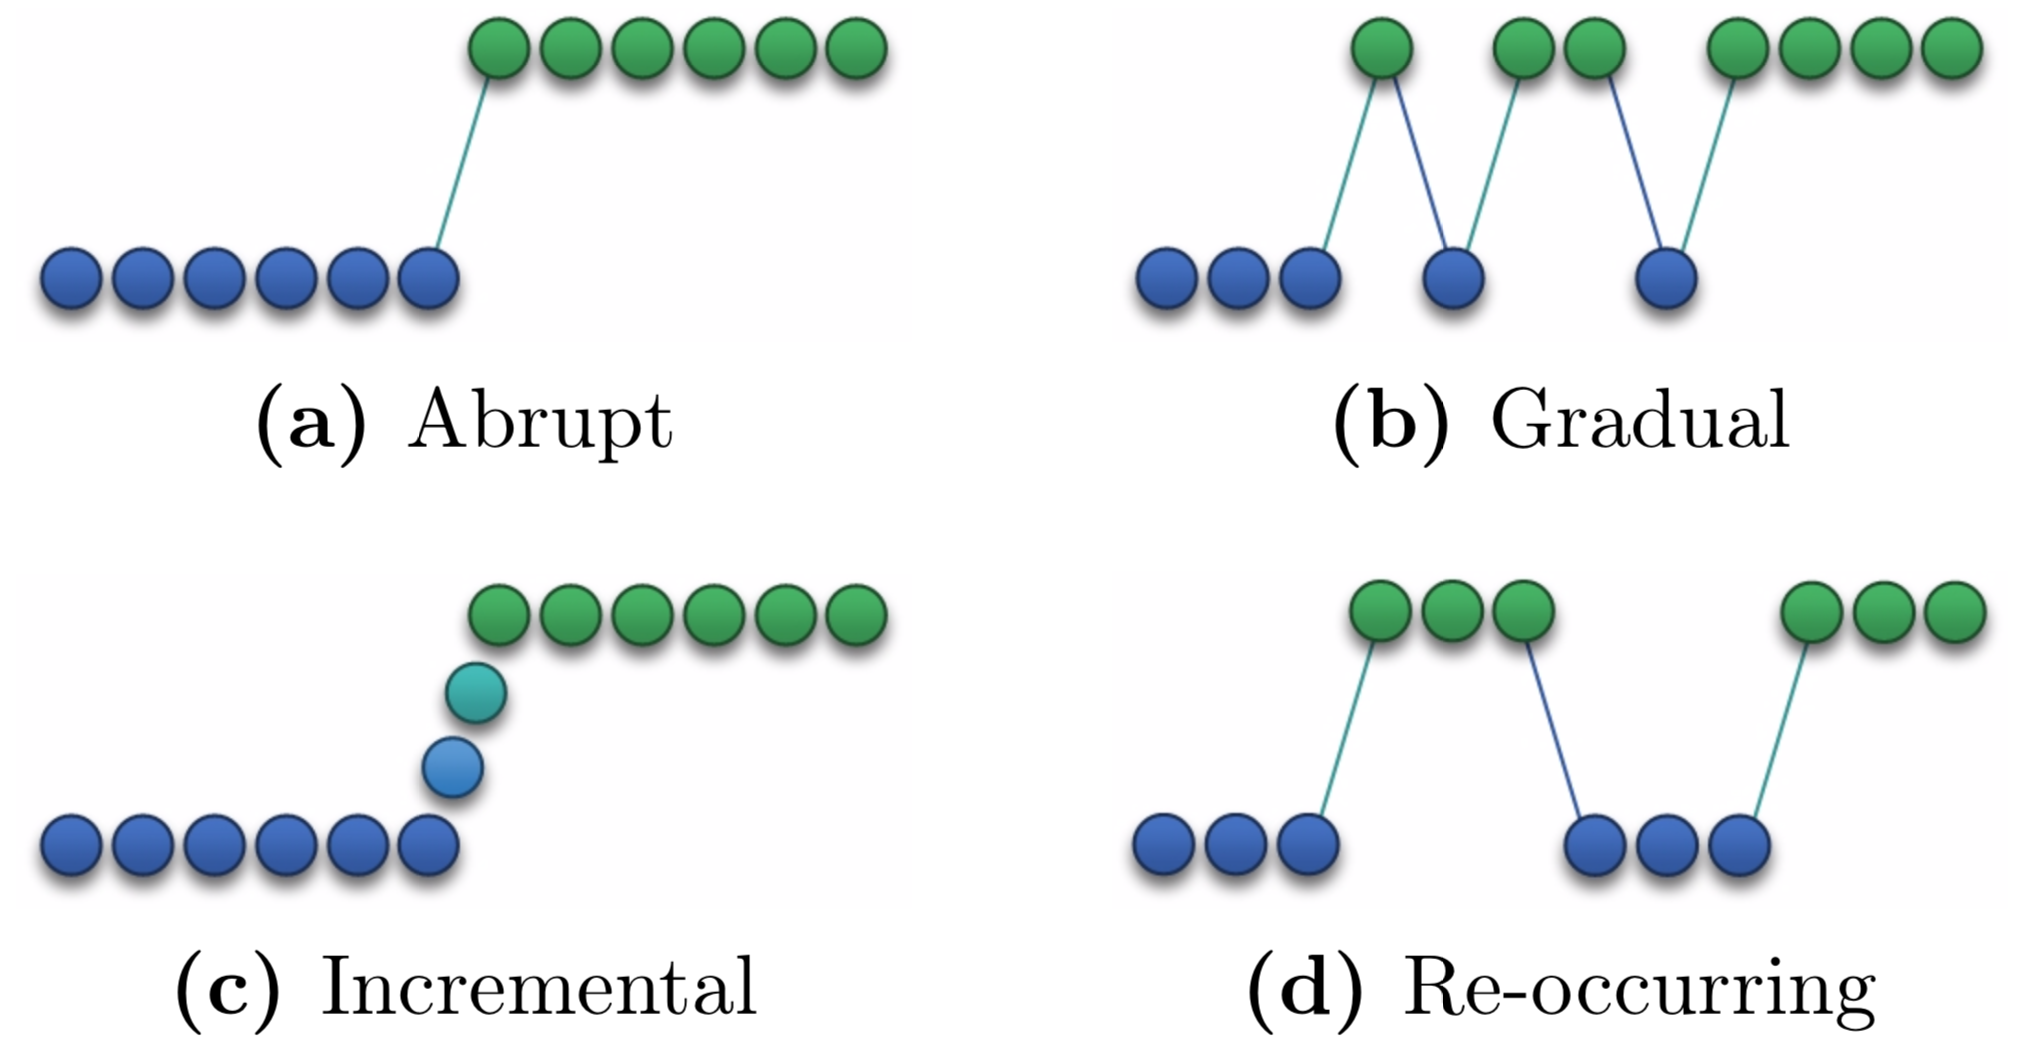
\includegraphics[width=\linewidth]{./images/chapter2/concept-drifts}
\caption{\label{fig:concept-drift-types}Types of drifts \cite{pesaranghader2018reservoirthesis}}
\end{figure}

\subsection{Concept Drift Detection Methods}
Methods to detect drifts do so based on information collected from a classifier's performance or directly from the incoming data. They warn that a drift may be occurring or that one has occurred, which is usually followed by updating, retraining or replacing an old classifier by a new one.

As we previously stated, fully supervised learning of data streams is not very suitable for real-world applications of data stream mining. It logically follows that drift detection methods that rely on a classifier's predictive performance, through the use of class labels, would also not be suitable for real-world applications.

3 metrics are usually considered to measure a drift detector's performance, according to \cite{KRAWCZYK2017132}: the number of correct positive drift detections (real drifts detected), the number of false alarms (no drift present, but detected one erroneously), and the drift detection delay (time between a drift and its actual detection).
As is usually the case, trade-offs are typically made between the three metrics. However, some aggregated measures are proposed in the literature. One such measure is the \textit{acceptable delay length}, proposed by Pesaranghader and Viktor in \cite{pesaranghader2016fast}, that determines if a drift is a true positive by measuring the distance between where a drift is detected and its actual location.

Gama categorizes drift detection methods into 4 groups \cite{Gama:2014:SCD:2597757.2523813}, which we will briefly cover in the upcoming paragraphs. These four groups are \textit{Statistical Process Control} methods, \textit{Sequential Analysis} methods, methods that \textit{monitor distributions of 2 different time windows} and \textit{contextual approaches}.

Drift Detection Method (DDM), proposed by Gama in \cite{gama2004learning}, is the most well-known method for the first category. The main idea behind DDM is to monitor the number of errors a classifier makes when predicting. They use the assumption, which they back through statistical theory, that the error-rate should decrease if the distribution generating the incoming data does not change. Consequently, a change in distribution will increase the error rate. They set two thresholds for both warnings and drifts. If and when the warning level is reached, incoming instances are to be stored in a special window to be used to retrain the classifier if it ever reaches the drift level. If the drift level is not reached and that the error rate drops below the warning level, the window is forgotten, and the drift is considered as a false alarm. DDM is not an optimal candidate to be extended for semi-supervised tasks.

Early Drift Detection Method (EEDM) \cite{baena2006early} extends DDM to improve the detection of gradual drifts. Instead of monitoring the number of misclassifications, they monitor the distance between misclassifications.

Krawczyk, in \cite{KRAWCZYK2017132}, states that sequential probability ratio tests, such as the Wald test, are the basis for detectors that use a \textit{sequential analysis} method.
The Cumulative Sum approach (CUSUM) proposed by Page in \cite{page1954continuous}, computes a weighted sum of the last $k$ examples to detect significant changes in a specified parameter of the probability distribution.

Methods using Hoeffding's (HDDM) and McDiarmid's inequalities were proposed in \cite{frias2015online}. These methods use moving averages and weighted moving averages to detect when a statistic ($p$) deviates statistically far from its expected value. The authors use a normal distribution example where the warning would be at 95\% ($p$ differs from $\mu\pm 2\sigma$) and the drift level at 99\% ($p$ differs from $\mu\pm 3\sigma$). The algorithm generalizes to any distribution but requires a desired significance level $\alpha_W$ for warnings and $\alpha_D$ for drifts. The authors state that their two methods are independent of classifier choice, have $O(1)$ complexity for time and applicable to scenarios where "labels are harder to obtain". 

Adaptive Windowing (ADWIN2) proposed by Bifet\cite{bifet2007learning} maintains a window of variable size containing bits or real numbers. The size of the window grows when no change is apparent and shrinks when change is apparent. ADWIN requires $O(\log(W)$ update time and memory for a window size of $W$. Change is detected when two distinct sub-windows have a different average. The split index between these two sub-windows is considered as an indication of a drift. ADWIN is a very well known drift detection method, and the best-known method for \textit{monitoring distributions of 2 different time windows}.

As we have previously stated, these drift detection methods rely on timely access to labels which is not a realistic assumption in the real world.  Active-Learning is an approach that has not yet extensively researched, nor has the use of unlabelled data for detecting drifts.

Unsupervised detection of drifts can rely on, according to \cite{sobolewski2013concept}, non-parametric statistical tests such as the CNF Density Estimation test \cite{dries2009adaptive}, the multivariate version of the Wald–Wolfowitz test \cite{friedman1979multivariate}.
A two-sample Kolmogorov–Smirnov test, a Wilcoxon rank sum test, and a two-sample t-test can also be used to detect drifts in data distribution according to \cite{sobolewski2013concept, sheskin2003handbook}.

Our thesis contributes to the gap in research dealing with unsupervised drift detection by extending FHDDM, which we cover in the following section.

\subsubsection{FHDDM and FHDDMS\label{section:fhddm/s}}
Ali Pesaranghader, in \parencite{pesaranghader2018reservoirthesis,pesaranghader2018reservoir, pesaranghader2016fast}, proposes two similar concept drift detection algorithms. The first uses a single sliding window, the other using two sliding windows: one short and the other longer. The sliding window stores whether or not the classifier predicted the class properly. His drift detection algorithms keep track of the maximum frequency value seen of correct predictions as well as the current frequency of correct predictions over the sliding window(s), then computes the difference between the maximum and current frequency. Hoeffding's inequality is used to determine the maximum desired difference between an empirical mean and a true mean of \textit{n} random independent variables, without making any assumptions on the distribution of the data. A drift is detected by using Hoeffding's inequality to detect when a significant change occurs between the two frequency measures, meaning that the difference surpasses a given threshold. The author found that FHDDM and FHDDMS were able to detect drifts with smaller delays and greater accuracy when compared to the state-of-the-art. Refer to algorithm \ref{alg:fhddm} for the implementation of FHDDM.

\begin{algorithm}
\caption{Fast Hoeffding Drift Detection Method (FHDDM)\label{alg:fhddm}}
\Fn{init(window\_size, delta)}{
    (n, $\delta$) = (window\_size, delta)\;
    $\epsilon_d = \sqrt{\frac{1}{2n}ln\frac{1}{\delta}}$\;
    reset()\;
}

\Fn{reset()}{
    w=[]\;
    $\mu^m=0$\;
}

\Fn{detect(p)}{
    \If{w.size = n}{
        w.tail.drop()\;
    }
    w.push(p)\;
    \eIf{$w.size < n$}{
        return False\;
    }{
        $\mu^t=\frac{w.count(1)}{w.size()}$\;
        \If{$\mu^m < \mu^t$}{
            $\mu^m =\mu^t$\;
        }
        $\Delta\mu = \mu^m - \mu^t$\;
        \eIf{$\Delta\mu \ge \epsilon_d$}{
            reset()\;
            \Return True
        }{
            \Return False
        }
    }
}
\end{algorithm}

%----------------------------------------------------------------------------------------

\section{Summary and Discussion}
 
% Chapter 3
\chapter{Contributions} % Main chapter title

\label{Chapter3} % For referencing the chapter elsewhere, use \ref{Chapter3} 

%----------------------------------------------------------------------------------------

\section{Voting Classifier}
A voting classifier was extracted from the scikit-learn library and modified to handle classification in a streaming setting. There were two voting schemes previously implemented; the first was a "hard" vote, which uses the predicted class labels for majority voting; and a "soft" vote, which selects the label with the highest probability average. 
\textit{Big blurb on voting classifiers}

%----------------------------------------------------------------------------------------

\section{FHDDMS}

Additionally, this thesis builds upon my colleague's, Ali Pesaranghader, work \parencite{pesaranghader2016fast} in which he proposes a concept drift detection algorithm that uses a sliding window storing whether or not the classifier predicted the class properly. To detect the drift, the author uses Hoeffding's inequality to detect when a significant change occurs between the maximum probability of correct predictions and the most recent probability of correct predictions. The authors found that FHDDMS was able to detect a drift with a smaller delay and greater accuracy when compared to the state-of-the-art.

\textit{Bigger blurb on how FHDDMS works}

%----------------------------------------------------------------------------------------

\section{Improvements to voting classifier for concept drift}

As previously stated, the scikit-learn voting classifier implements two voting strategies: the first being "soft" voting and the second being "hard" voting. The former calculates the probability that one or many tuples belong to a given class label. The latter performs a majority voting, meaning that the class label with the highest number of votes will be chosen.
The "soft" voting strategy also requires that all classifiers in the voting ensemble be capable of outputting a probability associated to its class label prediction.

We implemented one additional voting scheme similar to the "soft" scheme in that it requires its classifiers to output a probability or confidence in the class label prediction. Our method uses a logistic function with a sigmoid curve function to weigh the probability, centered around seventy five percent (75\%) confidence.
Logistic functions have the following equation
\begin{equation}
    f(x)=\frac{L}{1+e^{-k(x-x_0)}}\\ 
    \label{eq:logistic_function}
\end{equation}
where \textit{e} is the natural logarithm base, \textit{$x_0$} is the x-value of the sigmoid's midpoint, \textit{L} is the curve's maximum value, and \textit{k} is the steepness of the curve.

The logistic function that we used, uses the following values for the variables listed above. $x_0=0.75$, $L=1$, and $k=11$. These values were selected based on the resulting graph for values of x between zero and one ([0;1]), which allowed us to assign almost no weight to predictions with a probability of under forty percent (40\%), and give more weight to predictions with a probability of over seventy five percent (75\%).

Our proposed voting strategy therefore computes the sum of this logistic function using the prediction of each classifier for each class label. See the following equation:
\begin{equation}
    \sum_{i=0}^{c} \frac{\frac{1}{1+e^{-11(p_i(X)-0.75)}}}{\frac{1}{1+e^{-11(0.25)}}}\\ 
    \label{eq:logistic_sum}
\end{equation}
where $c$ is the number of classifiers in the voting ensemble and $p_i(X)$ is the probability of classifier $i$ predicting that the tuple belongs to class X. We then divide by the maximum value for $p_i(X)$ to ensure that our sum covers all values from 0 to 1.

Another weighting equation is proposed to determine if it is possible to achieve similar results by using a different function that resembles the logistic sigmoid function presented above while being less computationally intensive.
The weighting function is seen in equation \ref{eq:sin_weight_fn} and the sum is seen in equation \ref{eq:sin_sum}. The plot of equation \ref{eq:sin_weight_fn} is almost identical to the plot of \ref{eq:logistic_function}, with a maximum difference of approximately 0.0183 over [0, 1].
\begin{equation}
    f(x)=sin^8(\frac{x*\pi}{2})
    \label{eq:sin_weight_fn}
\end{equation}
\begin{equation}
\sum_{i=0}^{c} sin^8(\frac{p_i(X)*\pi}{2})
    \label{eq:sin_sum}
\end{equation}
The sums presented in equations \ref{eq:logistic_sum} and \ref{eq:sin_sum} are calculated for each class label. The class label with the highest sum is thereafter selected as the winner in the vote, and we hope proves to be more accurate based on the importance of the weight of the predicted class probability.

%----------------------------------------------------------------------------------------

\section{Hybrid sliding-tumbling windows}
One of many issues in data stream data mining is execution time, in the sense that our algorithm must learn faster than tuples can arrive. In our case, we want to determine if we can delay training of some classifiers in our VE, and how it affects execution time and classifying performance, as well as drift detection.

We propose the following algorithm, also seen in figure \ref{alg:sliding_tumbling_windows}, titled \textit{Sliding-Tumbling windows for training the VE}.
Let the number of tuples (single tuple or chunk) used in the interleaved test-then-train loop iterations be \textit{number\_of\_tuples}, and let \textit{number\_of\_classifiers} be the number of classifiers in the voting ensemble (VE). The VE will have a window size of \textit{number\_of\_tuples}*\textit{number\_of\_classifiers}. At every iteration of the interleaved test-then-train loop, we will append the new tuples to the VE's window and train a single classifier in the VE. For the next \textit{number\_of\_classifiers - 1} iterations, we will train the remaining \textit{number\_of\_classifiers - 1} classifiers in the ensemble so that from the point of view of the VE, we are training and testing using sliding windows but from the point of each c classifier, we are training them using tumbling windows.

While not used for the same purpose, my colleague Sarah D'Ettore used the same sliding batches to improve CDC-Stream in her thesis \citep{d2016fine}. Figure \ref{fig:sliding_tumbling_windows}, taken from my colleagues' thesis, shows how the algorithm works for three (3) classifiers in the ensemble with a batch size of one (1) and a window size of three (3). Each classifier will only learn from the same coloured batch; meaning that at time \textit{t}, only a single classifier has enough tuples to learn from, but the others will learn at time \textit{t+1} and finally at time \textit{t+2}. Each classifier will be learning from what essentially is a tumbling window, from their point of view, just not all from the same one.

The motivation for this technique is to determine if we can spend less execution time training the classifiers and to investigate how progressively delaying training of some of classifiers in the VE affects concept drift detection and classification performance while also hopefully reducing execution time.

\begin{algorithm}
\KwIn{X, y}
\KwResult{at least one classifier in the VE was trained}
\eIf {classifiers never been trained yet}{
    classifierToFit = classifierList[index]\\
    index = index+1 modulo numberOfClassifiers\\
    classifierToFit.partialTrain(X, y)
}{
    \For{$classifier \in classifierList$}{
        classifier.partialTrain(X, y)
    }
}
\caption{Sliding-Tumbling windows for training the VE\label{alg:sliding_tumbling_windows}}
\end{algorithm}

\begin{figure}
  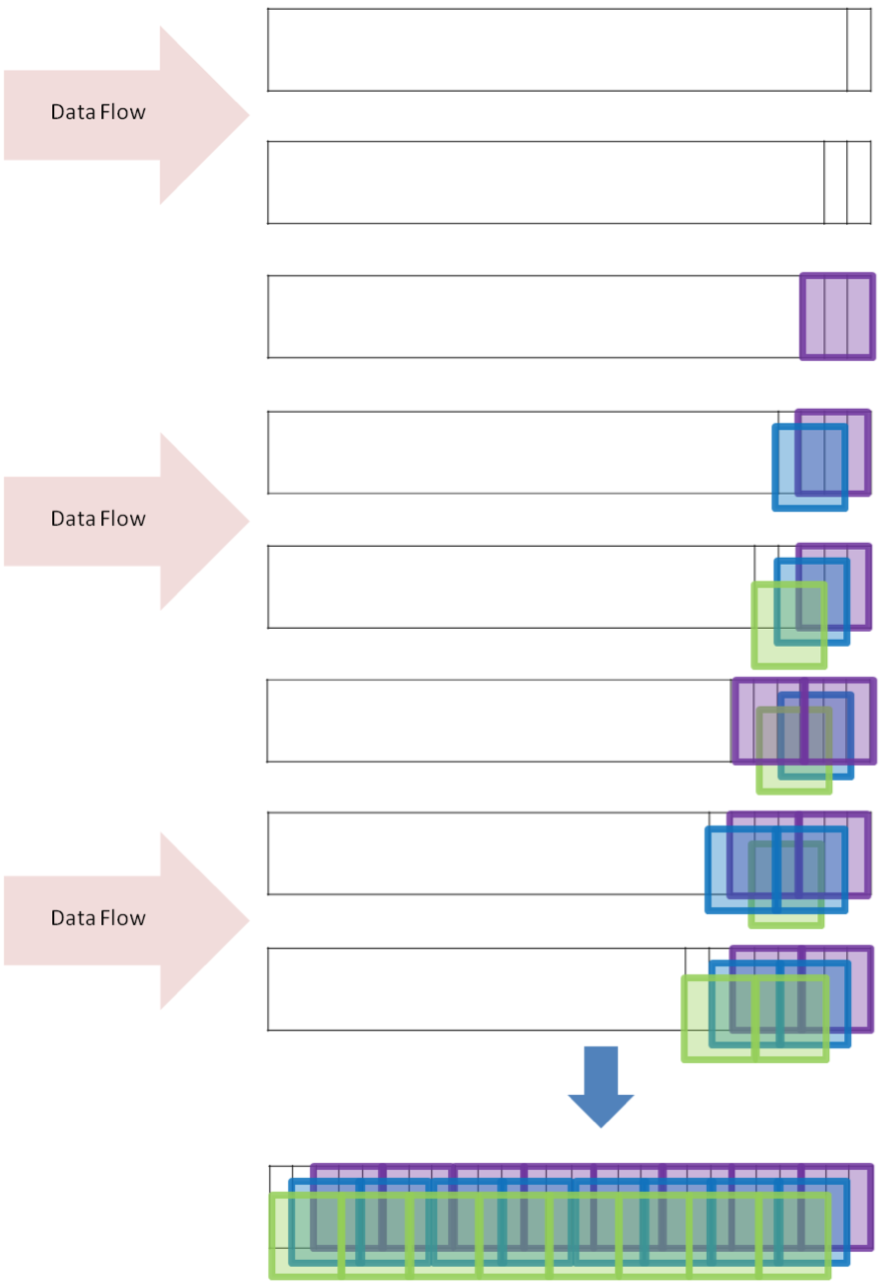
\includegraphics[width=\linewidth]{./Figures/sliding_tumbling_windows.png}
  \caption{Sliding Tumbling windows.}
  \label{fig:sliding_tumbling_windows}
\end{figure}



%----------------------------------------------------------------------------------------

\section{Improvements to voting classifier to reduce dependency on ground truth}

The interleaved test-then-train methodology in a data streaming setting has a rather large flaw: we are assuming that we obtain the ground truth immediately after testing. This means that we assume that the ground truth is always available in a fraction of a second after testing our models. For the large majority of cases, this approach is not realistic in a real world setting.

Therefore, we wanted to determine if we could re-use the idea behind self-training in an offline setting to reduce our dependency on the ground truth in the online streaming setting for the interleaved test-then-train method. We propose an approach that is, as previously stated, similar to self-training in that we use the classifier's prediction, and not ground truth, when training.

However, using only the predictions to train our model in an online setting is a recipe for disaster. The known cons to using self-training in an offline setting is that it can reinforce and classification errors; it is therefore a logical conclusion to assume that we will encounter the same risks in porting this idea to a streaming setting.

Given the restriction of limiting reinforcing misclassification errors, we want to determine at what ratio of predictions to ground truth our voting ensemble's accuracy would decline and by how much.

The algorithm behind this idea is very straightforward: it consists in duplicating the ground truth array, and replacing at random a particular fraction of values with the actual prediction from the classifier.

%----------------------------------------------------------------------------------------

\section{Improvements to FHDDMS to remove dependency on ground truth}

Along the same lines of the previous section, the drift detection algorithm proposed by my colleague Dr. Pesaranghader in \cite{pesaranghader2016fast}, \textit{FHDDMS}, relies on immediate knowledge of the ground truth after testing and after training. The drift detection mechanism in FHDDMS relies on storing, in a sliding window, whether or not the classifier accurately predicted the class. This method only applies to a select few domains where ground truth can be available almost instantly after the tuples are generated. For the large majority of domains, this method simply isn't applicable.

It is for that reason that we have set out to study how much ground truth can be omitted in the case of FHDDMS to reduce or remove its dependency on immediate knowledge of the ground truth to detect drifts in an online streaming setting.

In order to do so, we have opted to modify FHDDMS to run inside of the voting ensemble, with one sliding window per classifier in the ensemble. In each sliding window, we store not whether the classifier accurately predicted the class label, but rather if that sliding window's classifier voted for the class label that won the ensemble vote.

It is our hope that we can achieve similar results for drift detection speed while maintaining good classification accuracy.

%----------------------------------------------------------------------------------------

\section{Summary}

%----------------------------------------------------------------------------------------


\chapter{Experimental Design\label{chapter:experimental_design}} % Main chapter title
In this chapter, we describe our experimental design.

The data sets used for our analysis in the upcoming chapter are SEA \cite{street2001streaming}, CIRCLES, SINE1 and MIXED \cite{10.1007/3-540-59286-5_74}, which all containing noise, and either abrupt or gradual concept drifts.

The estimation technique we use is prequential evaluation, also known as interleaved test-then-train, which consists of infinitely executing a loop where a classifier first predicts labels for new data (without its label), then adapts its model for said data, with the correct label.

The performance measures that we use are the execution time, measured in seconds, as well as the $\kappa$-temporal statistic to evaluate a classifier's predictive performance, also called $\kappa^+$ or $\kappa_t$. This $\kappa$ statistic compares our classifier to a no-change classifier and takes into account temporal dependence in the data.

Using the mean values for the entire stream for both of the metrics mentioned above, we use statistical tests to determine whether or not the differences observed are statistically significant and not due to simple coincidence. When comparing two classifiers across multiple data sets, we use the Wilcoxon test, and when comparing more than two classifiers, we use the Friedman test, coupled with the post-hoc Nemenyi test.

We conduct the following experiments:
\begin{itemize}
\item  examine the impact of each parameter value on the mean of each metric,
\item rank the results of each parameter combination in order to establish any trend regarding parameter values across the metrics,
\item compare the top ranking parameter combinations to the state of the art.
\end{itemize}

%----------------------------------------------------------------------------------------

\section{Software and Hardware specifications}
In order to ensure that our experiments are reproducible, we specify the specifications of the hardware and software used to run them. All experiments were run on a MacBook Pro model \textit{11,4}. This machine was running macOS 10.14.4 on a quad-core Intel i7 2.2GHz processor (\textbf{3.4GHz} TurboBoost, 8 virtual cores), with a 256 GB SSD, and \textbf{16GB of RAM}. During the course of the experiments, the laptop was plugged in and fully charged.

Python 3.7.3 was installed, with the following dependencies:
\begin{itemize}
\item \textit{sortedcontainers} v2.0.5
\item \textit{numpy} v1.15.3
\item \textit{scipy} v1.1.0
\item \textit{scikit-learn} v0.20.0
\item \textit{pandas} v0.23.4
\item \textit{mlxtend} v0.13.0
\item \textit{scikit-multiflow} (latest commit from master rebased onto our branch) \textit{\textbf{\#f18a433}}
\end{itemize}

\section{Scikit-multiflow}
Scikit-multiflow \cite{skmultiflow} is a Python framework, that complements scikit-learn, an offline, batch learning Python library. As it currently stands, scikit-multiflow implements stream generators, machine learning algorithms, drift detection algorithms and evaluation methods for data streams. The authors describe scikit-multiflow as "an open-source framework for multi-output / multi-label and stream data mining", and takes its inspiration from MOA \cite{bifet2010moa} and MEKA \cite{read2016meka}. The former is the most popular data stream mining framework, implemented in Java, which includes a collection of machine learning algorithms, and evaluation tools. The latter is another project implemented in Java, but for multi-label learning and evaluation.

We selected this framework as it is backed by Bifet, implemented in Python: a popular language among data scientists, open-source, and very recent.

\section{Data sets\label{section:datasets}}
\subsection{Discussion on real-world and synthetic data sets}
The four data sets that we select to conduct our experiments on are known as benchmarking data sets for evaluating algorithms in evolving streams. As such, they are widely used in the literature \cite{baena2006early,bifet2007learning,gama2004learning,nishida2007detecting,olorunnimbe2015intelligent}. Lu, in a review on concept drift, states that "[as] instances are generated using predefined rules [...], synthetic data sets [are] a good option for evaluating the performance of learning algorithms in different concept drift scenarios" \cite[12-13]{lu2018learning}.

Real-world streaming data sets can present real concept drift, or drift that is synthetically generated. In the case of the latter, they have been referred to as semi-real-world streaming data sets \cite[42]{pesaranghader2018reservoirthesis}. While real data sets can provide realistic benchmarking for different drift detection algorithms, some researchers have put forward that the location and/or presence of concept drift for real-world streaming data sets are unknown \cite{bifet2007learning, bifet2009new,frias2015online,huang2015drift}. As such, real-world data sets make it difficult for algorithms to "understand the drift, and could introduce bias when comparing different machine learning models" \cite[13]{lu2018learning}. Lastly, as real-world data is time-consuming to correctly label, streaming data sets that contain real data are minuscule compared to synthetic data sets. It is not uncommon for real data sets to contain as little as five to ten thousand instances, which is a far cry from being realistic. As Bifet states in \cite{bifet2009new}, "demonstrating systems only on small amounts of data does not build a convincing case for capacity to solve more demanding data stream applications".

Therefore, we opt to conduct our experiments on the widely-used synthetic benchmarking data sets described below. Having said that, further research should still be conducted to investigate the performance of this framework on real, or semi-real streaming data sets.

\subsection{Synthetic Data Sets}

For our experiments, four synthetic data sets are used, three of which ($CIRCLES$, $SINE1$, and $MIXED$) were generated by my colleague for his paper \cite{pesaranghader2016fast} where he proposed FHDDMS, the drift detection algorithm. These data sets were generated with ten percent (10\%) class noise to test the robustness of his drift detection algorithm against noisy data streams. In order to do so, the true label of an instance is replaced by another label. The data sets contain one hundred thousand rows belonging to one of two classes, and present either gradual or abrupt concept drift. To generate concept drift, Bifet's approach is used, where a sigmoid function defines "the probability that every new instance of the stream belongs to the new concept after the drift" \cite{bifet2009new}. A parameter, $W$, indicates the length of the concept drift, starting at the point of change $t_0$. Pesaranghader sets $W=500$ for generating gradual concept drifts, and $W=50$ for abrupt drifts.
While the specific data sets we use were generated by Pesaranghader, the genesis of these synthetic data sets can be traced back to \cite{10.1007/3-540-59286-5_74} and were further used in, among others, the following papers \cite{baena2006early,bifet2007learning,gama2004learning,nishida2007detecting,olorunnimbe2015intelligent}. 

\subsubsection{CIRCLES}
As stated by Gama et al. in \cite{gama2004learning}, this data set is composed of two relevant numerical attributes: $x$ and $y$, which are uniformly distributed in [0, 1]. There are four different concepts in this data set, each representing whether or not a point is within a circle given $x$, and $y>$ coordinates for its centre and its radius $r_c$. This data set contains gradual concept drifts that occur at every twenty-five thousand (25 000) instances. The four pairs of $<(x,y), r_c>$ defining each concept are given in table \ref{table:circle_concepts}.

\begin{table}[]
\centering
\caption{\label{table:circle_concepts}$CIRCLES$ data set concepts}
\begin{tabular}{|c|c|c|c|c|}
\hline
center & (0.2, 0.5) & (0.4, 0.5) & (0.6, 0.5) & (0.8, 0.5) \\ \hline
radius & 0.15       & 0.2        & 0.25       & 0.3        \\ \hline
\end{tabular}
\end{table}

\subsubsection{SINE1}
As stated by Gama et al. in \cite{gama2004learning}, this data set contains abrupt concept drifts, with noise-free examples. It has only two relevant numerical attributes, for which the values are uniformly distributed in [0, 1]. Before the concept drift, all instances for values below the curve $y = sin(x)$ are classified as \textbf{positive}. Then, after the concept drift, the rule is reversed; therefore the values below the curve become \textbf{negative}. The drifts were generated at every twenty thousand (20 000) instances.

\subsubsection{MIXED}
As stated by Gama et al. in \cite{gama2004learning}, this data set contains abrupt concept drifts and uses four relevant attributes. Two of which are boolean, let them be $v$ and $w$; and the other two attributes are numerical, in [0, 1]. Instances belong to the positive class if two of three conditions are met: $v$ is true, $w$ is true, $y < 0.5 + 0.3 \times sin(3\pi x)$. For each concept drift, the conditions are reversed, meaning that if the conditions are met, it will be a positive instance, then after the drift, it will be a negative instance. The abrupt concept drifts occur at every twenty thousand (20 000) instances.

\subsubsection{Streaming Ensemble Algorithm (SEA) generator}
First described in \cite{street2001streaming} by Street and Kim, the Streaming Ensemble Algorithm (SEA) generates streams with abrupt concept drift. It is composed of three numerical attributes of values in [0, 10], and only the first two attributes are relevant. For each instance, the class is determined by checking if the sum of the two relevant attributes passes a threshold value. Let $f_1$ and $f_2$ be the two numerical relevant attributes, and $\theta$ the threshold. An instance belongs to class \textit{one} if $f_1 + f_2 \leq \theta$. As in Street's paper, our stream has four concepts, with the threshold values for each being 8, 9, 7 and 9.5. We generate streams of one hundred thousand instances, from zero to twenty percent noise, in ten percent increments ($\{0; 10; 20\%\}$). Drifts, therefore, occur at every twenty-five thousand (25 000) instances, and the length of the concept drift is $W=0$.

\section{Estimation techniques}
In an offline setting, with static data, the most common evaluation method used is called cross-validation. However, given how little time a model has to learn from each instance due to the velocity of data streams and the risk of concept drift, cross-validation is not suited for an online setting. The two following techniques are, though.

\subsection{Holdout}
Two distinct data sets are required for this technique: a training data set to train a model, and another to test it.  Cross-validation is typically used in offline static data mining, but is too computationally heavy and/or can be too time-consuming in a streaming setting, and therefore the validation step is skipped, and performance is measured against a single holdout set \cite{bifet2009data}.
 
This technique is most useful when the training and testing sets have already been defined, as it makes comparing results from different studies possible.
In order to track performance, the model is evaluated periodically, but not too frequently to avoid negatively impacting performance.

The holdout data set can be sourced from new tuples arriving from the data stream, and can also be added later to the training set in order to optimise instance use.

It should be sufficient to safely use a single static holdout set if we make the assumption that there is no concept drift \cite{bifet2009data}.

\subsection{Interleaved test-then-train, or prequential\label{section:prequential}}
Another evaluation method is prequential evaluation, also known as the interleaved test-then-train method. The evaluation method consists of first testing the classifier on a given set of instances, then training the classifier on that same set. The evaluation strategy, therefore, ensures that the model has not previously seen testing tuples, and no holdout testing set is necessary, and the accuracy of the model is therefore incrementally updated. This method also allows us to use all of the data for both testing and training. As more data is tested than in the holdout method, each instance used to assess the accuracy and performance of the model weighs less than it would have in a smaller holdout test set \cite{bifet2009data}.

All experiments are done using the interleaved test-then-train evaluation technique.

\section{Performance measures\label{section:performance_measures}}

\subsection{Accuracy \& Confusion Matrix}
Let us assume that we are dealing with a binary classification problem (with two classes) with a \textbf{P}ositive and \textbf{N}egative class.

A confusion matrix keeps track of the correctness of our classifying model by using the following four measurements \cite[77-79]{japkowicz2011evaluating}.

\begin{itemize}
\item False Positive (FP): number of instances incorrectly classified as positive
\item False Negative (FN): number of instances incorrectly classified as negative
\item True Positive (TP): number of instances correctly classified as positive
\item True Negative (TN): number of instances correctly classified as negative
\end{itemize}

It should then be clear that all of the positive class instances (P) are in the combined groups of FN and TP, and that all of the negative class instances (N) are in the remaining FP and TN groups.

A confusion matrix helps us to visualise these measurements by presenting them in a matrix (two-by-two grid in the case of a binary classification problem). Each column represents all of the instances for an actual class, whereas each row represents the instances predicted for a given class. Table \ref{table:confusion_matrix} shows a confusion matrix.

\begin{table}[]
\centering
\caption{Confusion Matrix\label{table:confusion_matrix}}
\begin{tabular}{|c|c|c|}
\hline
                   & Actual Positive & Actual Negative \\ \hline
Predicted Positive & TP              & FN              \\ \hline
Predicted Negative & FP              & TN              \\ \hline
\end{tabular}
\end{table}

Given our four measurements above, we can calculate the following metrics:
\begin{itemize}
\item The \textit{sensitivity} and \textit{specificity} (or \textit{recall}) indicate the completeness for a given class of instances retrieved that belong to that class \cite[96]{japkowicz2011evaluating}; in other words the percentage of correctly classified instances of a given class that were found overall.
\begin{equation}
\frac{TP}{TP+FN}=\frac{TP}{P} \text{ and } \frac{TN}{TN+FP}=\frac{TN}{N}
\end{equation}
\item The \textit{accuracy}, while not a reliable metric, indicates the number of correct predictions over all cases to be predicted \cite[86]{japkowicz2011evaluating}.
\begin{equation}
sensitivity\times\frac{P}{P+N}\times specificity\times\frac{N}{P+N} = \frac{TP+TN}{P+N}
\end{equation}
\item \textit{Precision} indicates the exactness of predictions for a given class \cite[99]{japkowicz2011evaluating}. In other words, the percentage of instances the classifier predicted as positive that were actually positive,\begin{equation}\frac{TP}{TP+FP}\end{equation}
\item \textit{F-measure}, which is the harmonic mean of precision and recall \cite[103]{japkowicz2011evaluating}. \begin{equation}2\times\frac{precision\times recall}{precision+recall}\end{equation}
\end{itemize}

\subsection{Kappa ($\kappa$) statistics\label{section:kappa_stats}}
\subsubsection{$\kappa$ statistic}
Bifet and Frank argue in \cite{bifet2010sentiment} that prequential accuracy is not well suited for classifying unbalanced data in a stream whereas the Kappa ($\kappa$) statistic proposed by Cohen in \cite{cohen1960coefficient} is better adapted when dealing with changing class distributions. They therefore proposed a sliding-window kappa as defined by equation \ref{eq:kappa}
\begin{equation}
\kappa=\frac{p_0-p_c}{1-p_c}
\label{eq:kappa}
\end{equation}where $p_0$ is the classifier's prequential accuracy and $p_c$ is the probability that a chance (or no-change) classifier makes a correct prediction. Refer to \cite{bifet2010sentiment} for the equations used to calculate $p_0$ and $p_c$.

Values of $\kappa$ are in [0, 1]. If the classifier always classifies instances correctly, then $p_0=1$ and $\kappa=1$; if the classifier correctly classifies instances as often as the chance classifier, then $p_0 = p_c$ and $\kappa=0$; and if the chance classifier is always right, then $p_c=1$ and $\kappa=1$.

\subsubsection{$\kappa^+$ statistic\label{section:kappa_t}}
The $\kappa^+$ statistic is an improvement upon the regular $\kappa$ statistic that takes into account temporal dependence in order to better evaluate the performance of a given classifier. When there is no temporal dependence in the data and that classes are balanced, then $\kappa^+$ is equal to $\kappa$. While we could solely rely on $\kappa^+$, the authors however recommend using both $\kappa$ and $\kappa^+$ statistics in order to obtain a more thorough evaluation.
$\kappa^+$ is defined in equation \ref{eq:kappa_plus}
\begin{equation}
\label{eq:kappa_plus}
\kappa^+=\frac{p_0-p'_e}{1-p'_e}
\end{equation}where $p_0$ is the classifier's prequential accuracy and $p'_e$ is the accuracy of a no-change classifier. The no-change classifier predicts that the next class label will be the same as the last seen class label \cite{bifet2015efficient}. Just like the original $\kappa$ statistic, $\kappa^+\in [0, 1]$. Refer to \cite{DBLP:conf/pkdd/2013-1} for the equations relating to calculating $p_0$ and $p'_e$. $\kappa^+$ is also sometimes referred to as $\kappa$-temporal ($\kappa_t$) \cite{vzliobaite2015evaluation}.

\subsubsection{$\kappa_m$ statistic}
The $\kappa_m$ statistic is another improvement upon the regular to indicate whether a classifier is performing better than a majority-class classifier \cite{bifet2015efficient}. Its definition is given in equation \ref{eq:kappa_m}.

\begin{equation}
    \label{eq:kappa_m}
    \kappa_m = \frac{p_0-p_m}{1-p_m}
\end{equation}where $p_0$ is the classifier's prequential accuracy and $p_m$ is the prequential accuracy of a majority-class classifier. If the classifier always predicts correctly, then $\kappa_m=1$. If the classifier predicts correctly as often as the majority-class one, then $\kappa_m=0$.

\subsection{Testing for Statistical Significance}
While the measures presented in \ref{section:performance_measures} are useful for evaluating the performance of our classifiers, it is insufficient to rely solely on them to fully evaluate performance differences between classifiers. Statistical significance tests are used to determine whether or not the differences that were observed are statistically significant and not due to simple coincidence \cite{japkowicz2011evaluating}.

Popular choices for statistical tests in the machine learning community for comparing multiple classifiers across multiple cases are the Analysis of Variance (ANOVA) \cite{fisher1956statistical} and the Friedman test \cite{friedman1937use}. 

The ANOVA test assumes a normal data distribution whereas the Friedman test does not. It is for this reason, coupled with the fact that the Friedman test is also non-parametric, that we have chosen the latter as our choice for a statistical significance test. However, the Friedman test is not recommended when only comparing two algorithms on multiple domains \cite[355]{flach2012ml}; for that reason, we will be using the Wilcoxon test \cite{wilcoxon1945individual} in those scenarios.

\subsubsection{The Friedman test}
The test ranks each algorithm separately for each data set and computes a test statistic using the variation within the ranks and the variation within the error variation. The Friedman statistic $\chi^2_F$ is defined in equation \ref{eq:friedman_statistic}, taken from \cite{japkowicz2011evaluating};

\begin{equation}
\label{eq:friedman_statistic}
\chi^2_F = \frac{SS_{Total}}{SS_{Error}}=\bigg[\frac{12}{n\times k\times(k+1)}\times\sum_{j=1}^k(R_.j)^2\bigg]-3\times n \times (k+1)
\end{equation}where $n$ is the number of data sets, $k$ is the number of algorithms considered, and $R$ simply denotes ranking. And finally $(k-1)$ is known as the degrees of freedom.

The Friedman statistic ($\chi^2_F$) is then looked up in the $\chi^2$ distribution table to obtain a \textit{probability value} (p-value), signifying $P(\chi^2_{k-1} \geq \chi^2_F )$. This p-value is widely used in null-hypothesis testing by measuring it against a threshold value called a significance level. A lower p-value means a higher statistical significance. Traditionally, the significance level is either 0.1 or 0.5, and denoted as $\alpha$. The null hypothesis is accepted if the p-value is greater than $\alpha$; otherwise, $H_1$ is accepted, and the null hypothesis is rejected.

When the null hypothesis is rejected following a Friedman test, post hoc Nemenyi tests are recommended by Japkowicz and Shah in \cite{japkowicz2011evaluating}, as well as Flach in \cite[355]{flach2012ml}.

\subsubsection{Wilcoxon's Signed-Rank test}
This test is a non-parametric version of the matched-paired \textit{t}-test. It is used to test if two paired samples come from the same distribution, by measuring the difference in their mean ranks.

The test procedure is as follows \cite[233-235]{japkowicz2011evaluating}, \cite[354]{flach2012ml}:

$N$ will be set as the sample size, meaning that there are $2N$ data points, and since data are paired, $[x_{1, i}, x_{2, i}]$ represent the measurements for pairs where $i\in [1 ; N]$.

We test the following null hypothesis.

$H_0 $: difference between the pairs follows a symmetric distribution around zero
\newline$H_1$: does not follow a symmetric distribution around zero

\begin{itemize}
\item Calculate $d_i = (x_{1, i} - x_{2, i}) \forall i\in[1;N]$.
\item Pairs for which the difference is zero are excluded, let $N_r$ be the reduced sample size.
\item Rank the $N_r$ pairs by their absolute difference in increasing order, let $R_i$ denote rank. In the case of ties, assign the pairs with the average of their ranks.
\item Two sum of ranks are then calculated: 
\newline$W_{s 1}=\sum_{i=1}^{N_r} I(d_{i}>0) \operatorname{rank}(d_{i}),$ 
\newline$W_{s 2}=\sum_{i=1}^{N_r} I(d_{i}<0) \operatorname{rank}(d_{i})$.
\item Calculate statistic $T_{wilcox}=\min(W_{s 1}, W_{s 2})$.
\item For smaller values of $N$, which is the case in our thesis, look up tabulated critical values of $T$ (according to N and statistical significance level) and reject the null hypothesis if the statistic is inferior to the tabulated value.
\end{itemize}



\subsubsection{Post-hoc test: the Nemenyi test}
The Nemenyi test \cite{nemenyi1962distribution} is used in order to determine which algorithms compared in the Friedman test actually differ. It computes a statistic, $q$, as defined in equation \ref{eq:nemenyi_q} for a pair of classifiers $f_{j1}$ and $f_{j2}$. $q$ gives us the difference between ranks of the two algorithms, and can be also expressed as a critical difference (CD) \cite[356]{flach2012ml}. In order compare the rankings, the Nemenyi test computes the mean rank for a given classifier using equation \ref{eq:nemenyi_mean_rank} where $R_{ij}$ is the rank of classifier $f_j$ on data set $S_i$ \cite[256-257]{japkowicz2011evaluating}.
\begin{equation}
\label{eq:nemenyi_q}
\overline{R}_{.j}=\frac{1}{n}\sum_{i=1}^nR_{ij}
\end{equation}\begin{equation}
\label{eq:nemenyi_mean_rank}
q=\frac{\overline{R}_{.j1}-\overline{R}_{.j2}}{\sqrt{\frac{k(k+1)}{6n}}}
\end{equation}

\section{Experimental Setup}
For these experiments, the following classifiers were used: Gaussian Naive Bayes (G\_NB), Leveraging Bagging, Stochastic Gradient Descent (SGD), Multinomial Naive Bayes (M\_NB), and our Voting Ensemble composed of three sub-classifiers. The three classifiers inside the voting ensemble are the SGD, M\_NB, and G\_NB. Finally, we also used a no-change classifier as well as a majority-class classifier as our baselines.

Readers familiar with classification algorithms \cite{viktor2015course} might know that some advantages of NB are its scalability, high accuracy, ability to use prior knowledge, and the fact that it has comparable performance to decision trees and neural networks. NB is incrementally more confident, and easy to implement. However, the downsides are its significant compute costs, and that using conditional dependencies reduces accuracy due to the real dependency between attributes.
SGDs have generally high predictive accuracy, generalise well meaning that they are robust and suitable for noisy domains, and good for incremental learning. However, they are known to have a slow training time, may fail to converge, and output a black box model which means that results cannot be interpreted.
Leveraging bagging \cite{bifet2010leveraging} is an improvement over the Online Bagging technique of Oza and Russel. They introduce more randomisation to the online bagging algorithm to achieve a more accurate classifier. However, the authors noted that subagging, half subagging, and bagging with-out replacement ran faster but were marginally less accurate.

Unless stated otherwise, our default parameters for the experiments are listed in table \ref{table:default_exp_parameters} and the default parameters for the classifiers are listed in table \ref{table:default_clf_parameters}. These values were obtained through extensive experimentation.

Finally, each experiment is run on five different examples each sourced from three synthetic data sets (5 examples of $SINE1$, another 5 of $CIRCLES$, etc.) and three streams generated by the SEA generator with levels of noise in increments of ten percent (from 0\% to 20\%), for a grand total of eighteen (18) streams of one hundred thousand (100000) instances.

\begin{table}[]
\centering
\caption{\label{table:default_exp_parameters}Default parameters for the experiments}
\begin{tabular}{|l|l|}
\hline
\multicolumn{1}{|c|}{\textbf{Parameter}} & \multicolumn{1}{c|}{\textbf{Value}} \\ \hline \hhline{==}
Classifier & Ensemble Voting Classifier \\ \hline
Pretrain size & 1 000 \\ \hline
Max samples & 100 000 \\ \hline
Batch size & 25 \\ \hline
Window size & 75 \\ \hline
Window type & sliding tumbling hybrid \\ \hline
Ground truth \% & 100 \\ \hline
Drift reset type & none \\ \hline
\end{tabular}
\end{table}

\begin{table}[]
\centering
\caption{\label{table:default_clf_parameters}Our default parameters for all classifiers}
\begin{tabular}{|l|l|}
\hline
\multicolumn{1}{|c|}{\textbf{Classifier}} & \multicolumn{1}{c|}{\textbf{Parameters}} \\ \hline \hhline{==}
Leveraging Bagging & \begin{tabular}[c]{@{}l@{}}base\_estimator=HoeffdingTree()\\ n\_estimators=10\\ w=6\\ delta=0.002\\ leverage\_algorithm=leveraging\_bag\\ random\_state=None\end{tabular} \\ \hline
Hoeffding Tree & \begin{tabular}[c]{@{}l@{}}max\_byte\_size=33.5MB\\split\_criterion=information gain\\split\_confidence=0.0000001\\binary\_split=False\\remove\_poor\_atts=False\\no\_preprune=False\\leaf\_prediction=Naive Bayes Adaptive\end{tabular} \\ \hline
Gaussian NB & \begin{tabular}[c]{@{}l@{}}priors=None\\ var\_smoothing=1e-9\end{tabular} \\ \hline
Multinomial NB & \begin{tabular}[c]{@{}l@{}}alpha=1.0\\ fit\_prior=True\\ class\_prior=None\end{tabular} \\ \hline
Stochastic Gradient Descent & \begin{tabular}[c]{@{}l@{}}loss=log\\ penalty=l2\\ alpha=0.0001\\ l1\_ratio=0.15\\ fit\_intercept=True\\ max\_iter=1000\\ tol=1e-3\\ shuffle=True\\ epsilon=0.1\\ n\_jobs=-1\\ random\_state=None\\ learning\_rate=optimal\\ eta0=0.0\\ power\_t=0.5\\ early\_stopping=False\\ validation\_fraction=0.1\\ n\_iter\_no\_change=5\\ average=False\\ n\_iter=None\end{tabular} \\ \hline
\end{tabular}
\end{table}

Our voting ensemble takes seven (7) different parameters, some of which are conditional upon the value of others. The parameters and the values they can take are shown in table \ref{table:ensemble_params}. Some combinations of parameters are not allowed such as combining boolean voting with non-boolean drift detector content, or using probability voting with weighted probability drift content. In the worst case, when counting the illegal combinations, there are $4\times2\times3\times5\times4\times3\times2=1880$ combinations. There are 1110 permitted parameter combinations.

\begin{table}[]
\caption{Voting ensemble parameters\label{table:ensemble_params}}
\begin{tabular}{|l|l|}
\hline
\textbf{Parameter} & \textbf{Values} \\ \hline \hhline{==}
Voting type & boolean, probability, avg. w. probability, w. avg. probability \\ \hline
Window type & sliding, hybrid \\ \hline
Chunk size & 25, 75, 100 \\ \hline
Ground truth & 60\%, 70\%, 80\%, 90\%, 100\% \\ \hline
Drift reset type & no drift detection, blind, partial, complete \\ \hline
Drift content & boolean, probability, weighted probability \\ \hline
Drift detector count & 1 or many \\ \hline
\end{tabular}
\end{table}

We will run our algorithm for each permitted combination of the parameters stated above, and will measure  $\kappa_t$ and the execution time for each of the eighteen data sets. We will then evaluate how each parameter affects the execution time and $\kappa_t$.

We will test the null hypothesis that all values of a given parameter will perform similarly in regards to a given measure when we set all other parameters. We will repeat this experiment over all combinations of the "other" parameters.

For parameters that have only two values, we will use the Wilcoxon test to determine if the values of the parameters lead to statistically significant differences in the metrics measured. We will also use the internal intermediate results of the Wilcoxon test to rank the parameter values, again depending on the metric measured.

Otherwise, for parameters that can take more than two values, we will use the Friedman test; and when the Friedman test rejects the null hypothesis, we will use a post-hoc Nemenyi test to determine which pairs of values lead to statistically significant differences in the measured metrics.

We will be comparing the values of each parameter across all permitted parameter combinations. We will then be able to assess if a parameter value is often ranked better and if it seems to influence the measures even when changing the "other" set parameters. In other words, we aim to determine if a parameter is likely to frequently affect our measured metrics no matter of the other parameters.

After we assess the impact of the parameter values on the measured metrics, we will use the ranking algorithm from the post-hoc Nemenyi test to rank each parameter combination to determine the top ranking combination for each measured metric and over both metrics.

Once we obtain the parameter combinations that lead to the best results, we will compare them to the state of the art algorithm (leveraging bagging). We will, also, be comparing these results with no-change and majority-class classifiers (trained with 100\% labelled examples and sliding windows). The leveraging bagging classifier is implemented with a built-in ADWIN drift detector. As we will be comparing at least 3 algorithms, we will employ the Friedman test in conjunction with the post-hoc Nemenyi test where appropriate to determine which pairs of algorithms differ.

In summary, we:
\begin{enumerate}
\item compare each value of one parameter (while setting other parameters to a given value), multiple times and each time changing the other parameter combination to assess the impact of that one parameter value on the measured metrics
\item rank the results of each parameter combination
\item use those rankings to compare the top parameter combinations to the state of the art
\end{enumerate}

In the following chapter, we present the results of our experiments, analyse these findings and discuss their significance. 
% Chapter 5

\chapter{Experimental Evaluation and Discussion} % Main chapter title

Recall from the previous chapter that in order to evaluate our contributions, we will need to compare how our algorithm performs against 4 different data sets. We will be using the $\kappa_t$ metric, as well as the execution time. Finally, we will also be considering the percentage of labelled data is used to train our ensemble.
{In this chapter, we will be investigating how each parameter influences each measured metric using omnibus Wilcoxon and Friedman tests, and in the case of the latter, post-ho\textbf{}c Nemenyi tests to further confirm which pairs of algorithms differ in performance. Next, we will compare all of the parameter combinations together by ranking them by each metric. This is done to find any trends that lead to better performance. Finally, we will compare our approach to the state of the art}

\label{Chapter5} % For referencing the chapter elsewhere, use \ref{Chapter3} 

\begin{figure}
  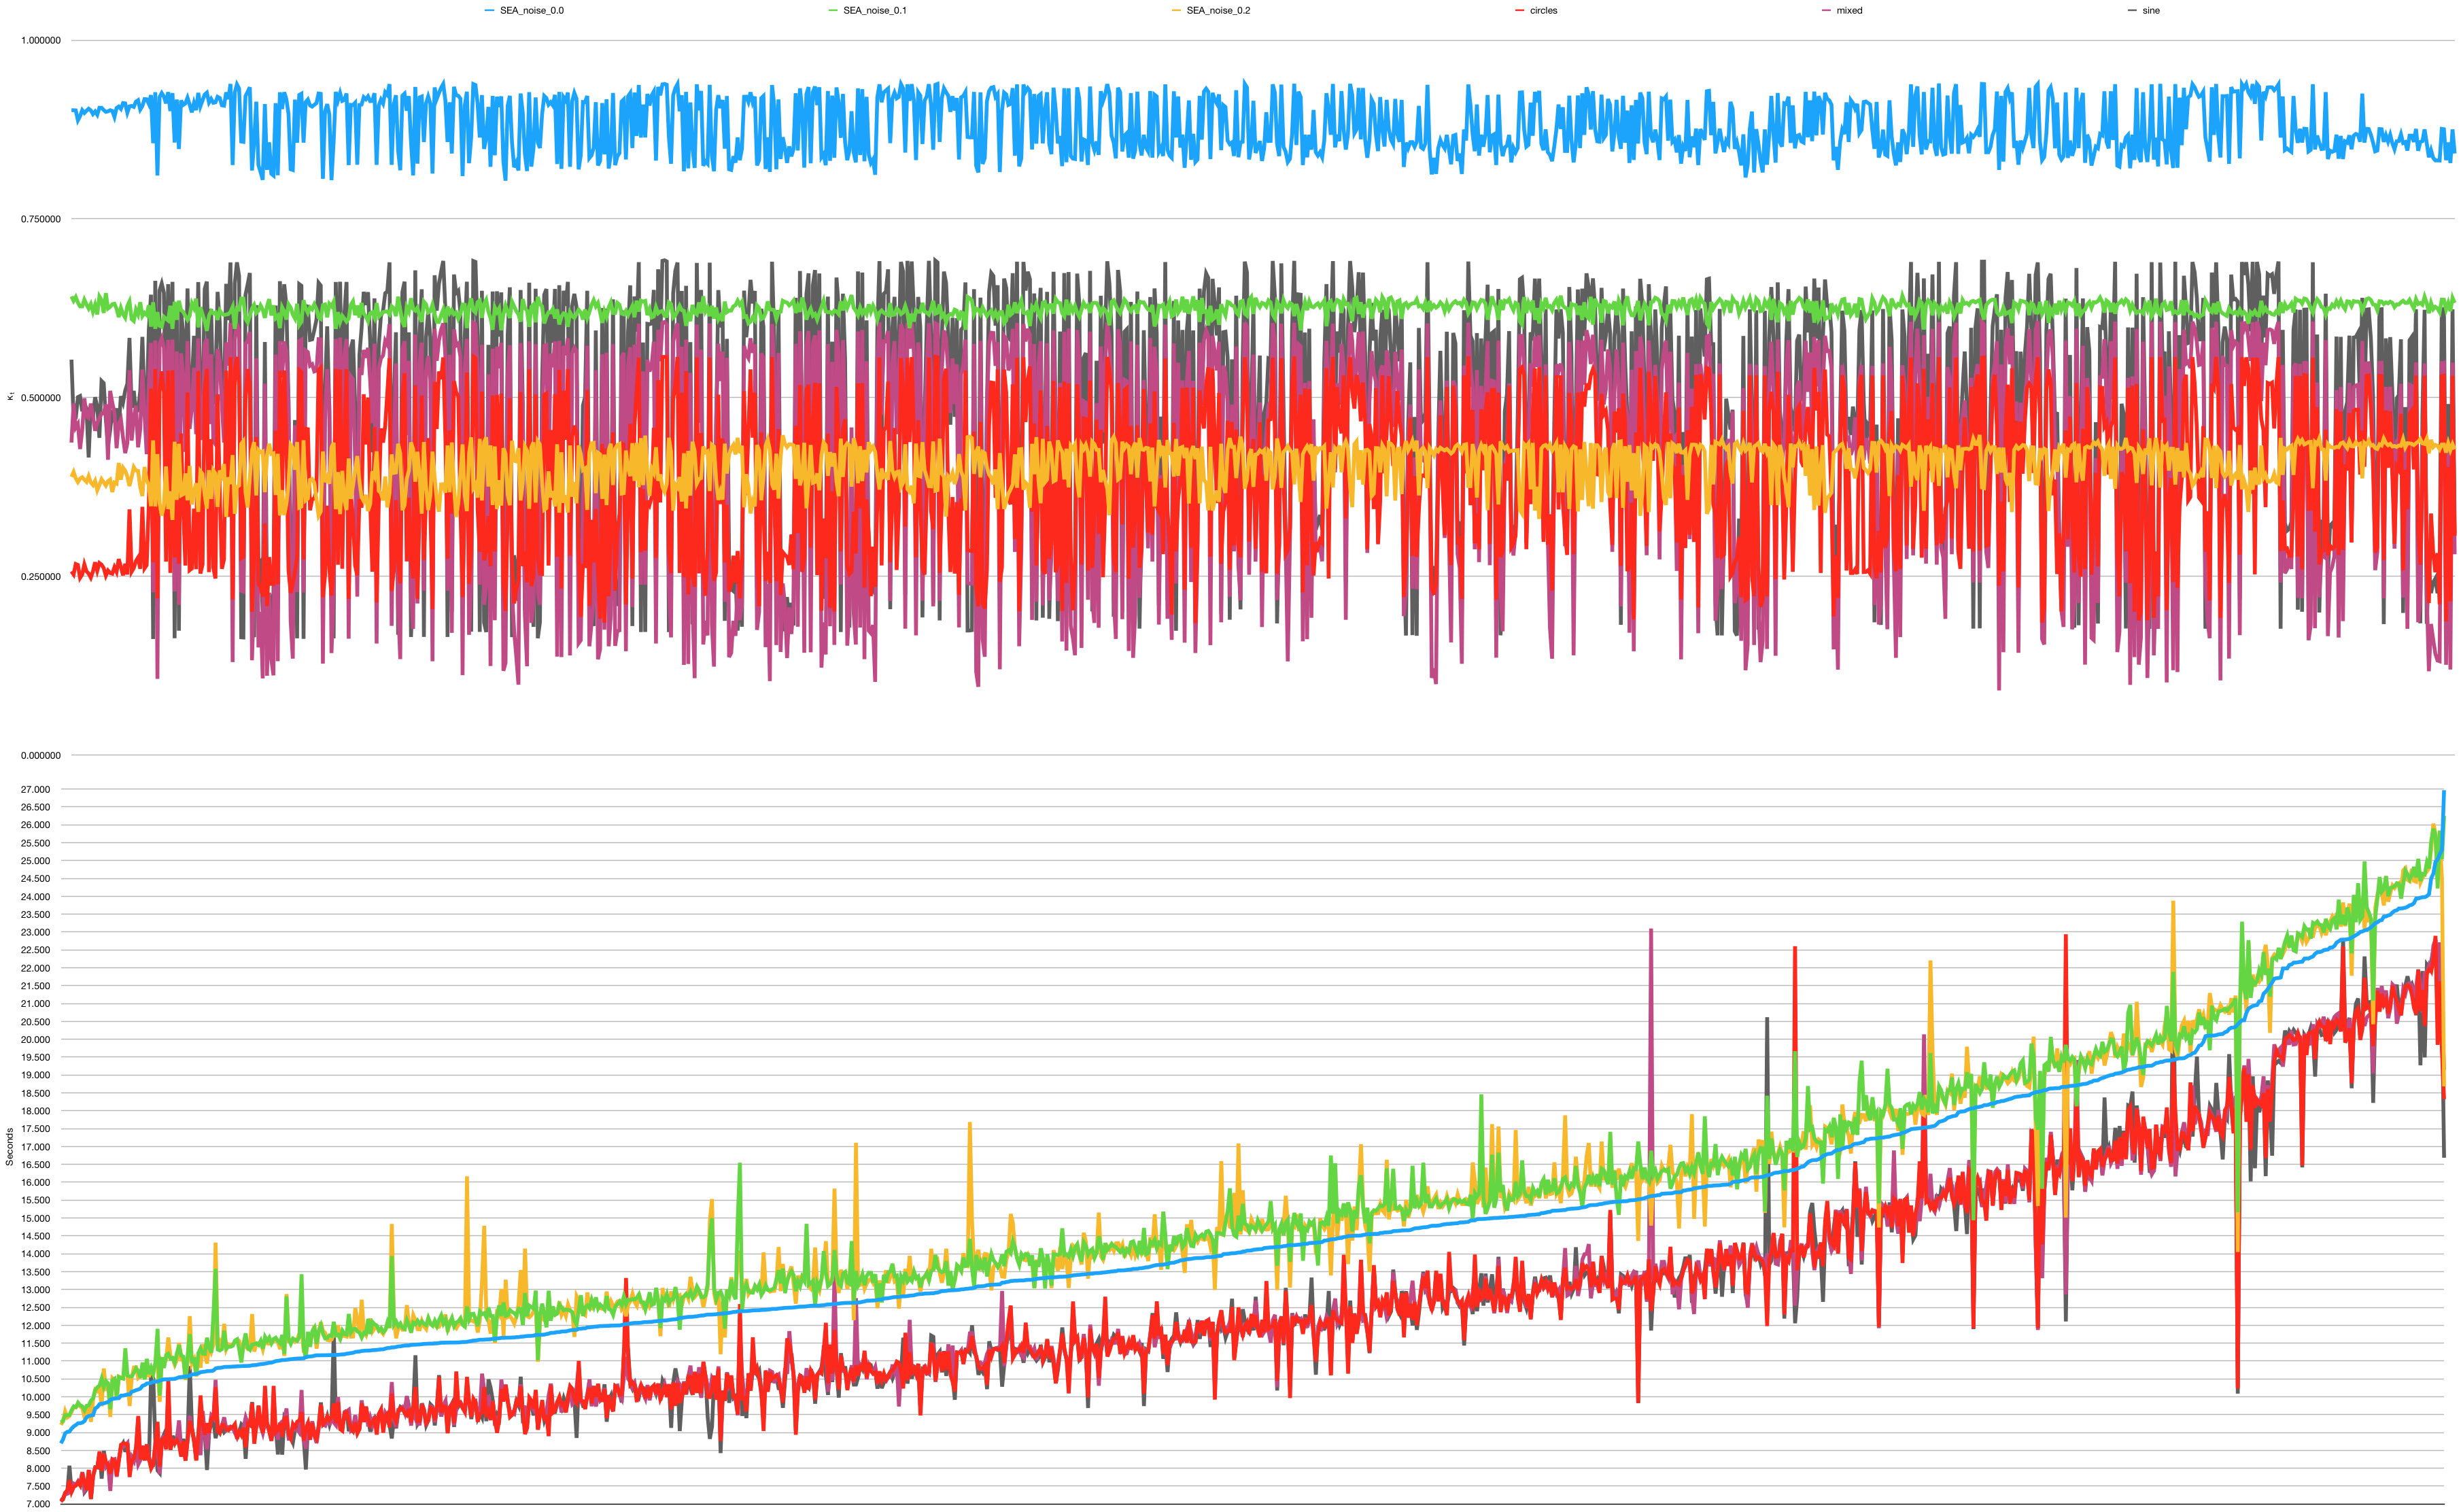
\includegraphics[width=\linewidth]{./images/kappa_vs_time}
\caption{\label{fig:kappa_vs_time}$\kappa_t$ in relation to time, across all parameter combinations}
\end{figure}
Figure \ref{fig:kappa_vs_time} shows that as the execution time increases, $\kappa_t$ stays roughly constant. The majority of the changes seem to be due to the various parameter combinations. This is a good sign as it suggests that the predictive accuracy of our model is at most very loosely tied to the execution time of its algorithm.

\section{Investigating how each parameter influences each metric}

\subsection{Wilcoxon tests}

\subsubsection{Drift Detector Count}

\begin{table}[]
\centering
\caption{\label{table:wilcoxon_significant}Statistically significant percentage of parameter combinations found via the Wilcoxon test}
\begin{tabular}{|l|l|l|l|l|l|}
\hline
\textbf{Parameter} & \textbf{Measure} & \textbf{0.05} & \textbf{0.01} & \textbf{0.001} & \textbf{Total} \\ \hline \hhline{======}
\multirow{2}{*}{Drift detector count} & execution time & 5\% & 6\% & 82\% & 93\% \\ \cline{2-6} 
 & $\kappa_t$ & 4\% & 1\% & 1\% & 7\% \\ \hline\hhline{======}
\multirow{2}{*}{Window type} & execution time & 1\% & 6\% & 89\% & 97\% \\ \cline{2-6} 
 & $\kappa_t$ & 7\% & 8\% & 44\% & 60\% \\ \hline
\end{tabular}
\end{table}

As we can see from table \ref{table:wilcoxon_significant}, the parameter \textit{Drift Detector Count} seems to heavily influence the execution time of the algorithm, regardless of the other parameter values. When it comes to the $\kappa_t$ metric, only 7\% of combinations proved to have statistically significant differences in predictive performance. 

\begin{table}[]
\centering
\caption{\label{table:wilcoxon_drift_detector_count}Statistically significant percentage of parameter combinations by parameter value for Drift Detector Count found via the Wilcoxon test}
\begin{tabular}{|l|l|l|l|l|l|l|l|l|}
\hline
\multirow{3}{*}{\textbf{Measure}} & \multicolumn{4}{l|}{\textbf{1 for ensemble}} & \multicolumn{4}{l|}{\textbf{1 per classifier}} \\ \cline{2-9} 
 & \multicolumn{2}{l|}{\textbf{significant}} & \multicolumn{2}{l|}{\textbf{insignificant}} & \multicolumn{2}{l|}{\textbf{significant}} & \multicolumn{2}{l|}{\textbf{insignificant}} \\ \cline{2-9} 
 & \textbf{count} & \textbf{\%} & \textbf{count} & \textbf{\%} & \textbf{count} & \textbf{\%} & \textbf{count} & \% \\ \hline \hhline{=========}
execution time & 447 & 99\% & 22 & 73\% & 4 & 0\% & 8 & 26\% \\ \hline
$\kappa_t$ & 19 & 59\% & 206 & 48\% & 13 & 40\% & 217 & 51\% \\ \hline
\end{tabular}
\end{table}


\begin{figure}
\centering
  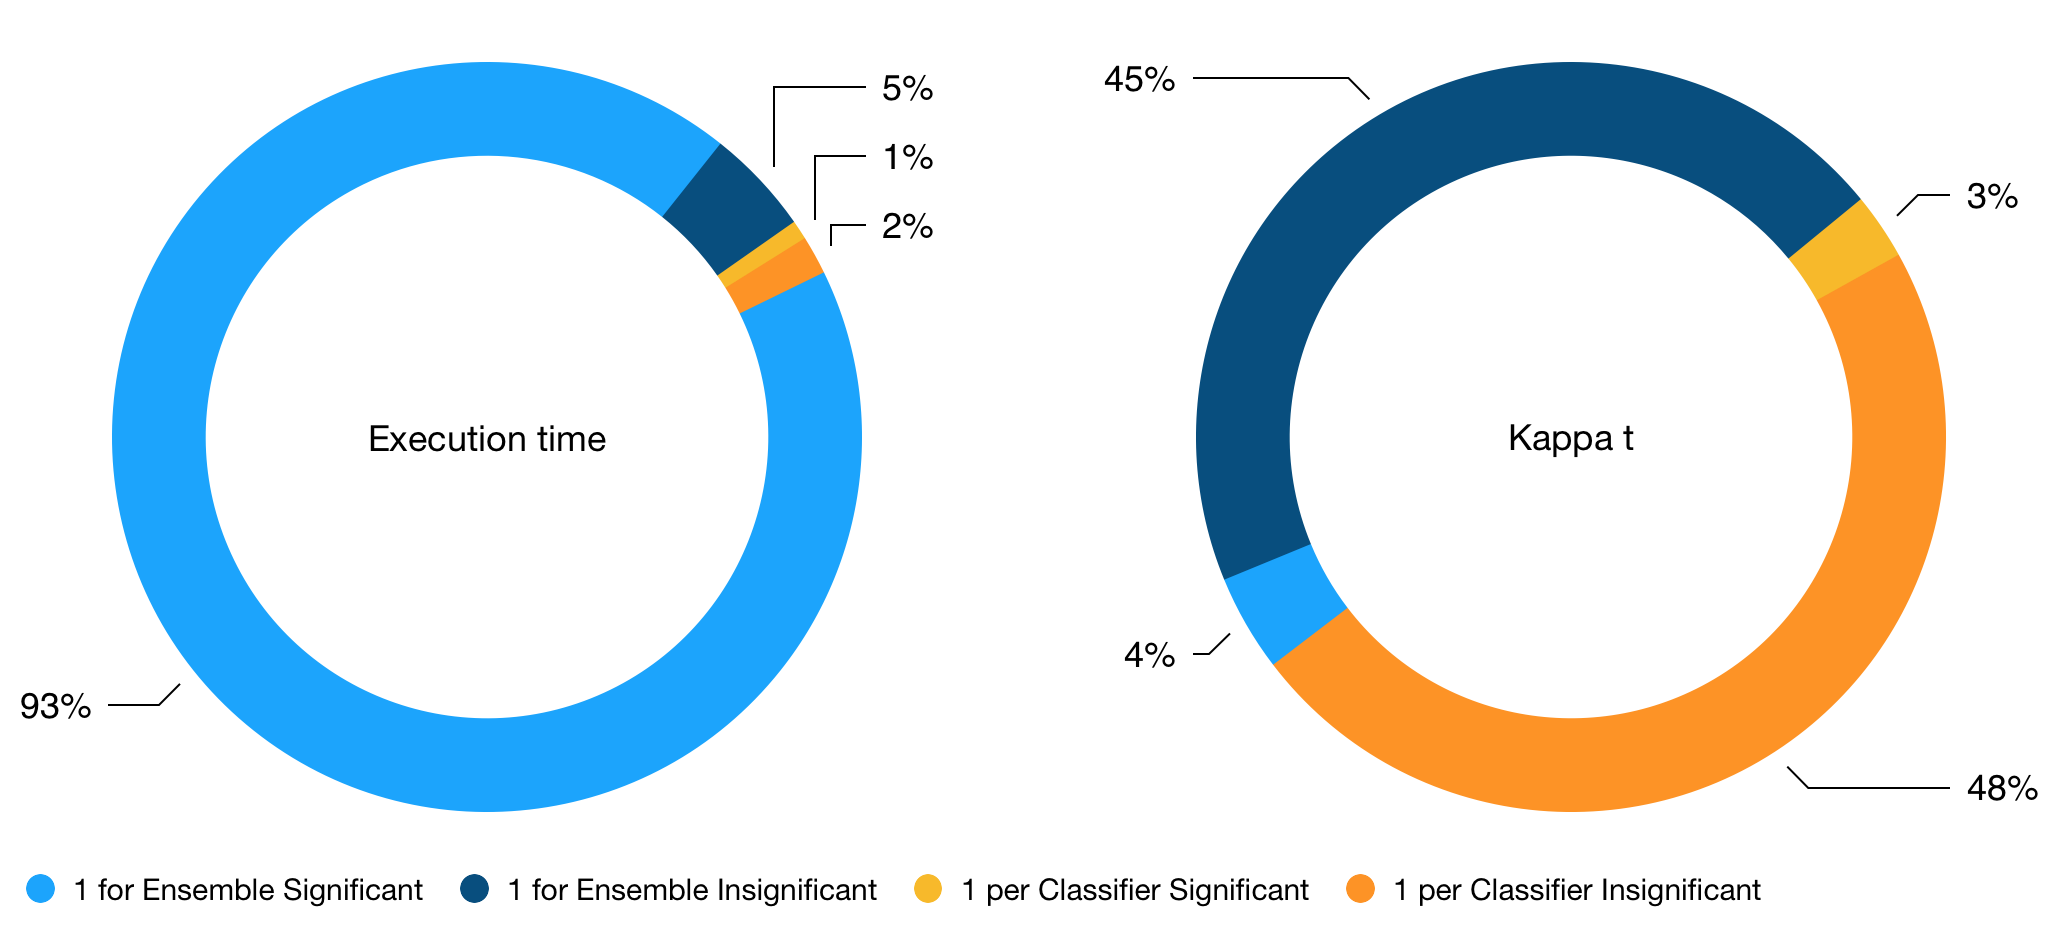
\includegraphics[width=\linewidth]{./images/wilcoxon_drift_detector_count_pie}
\caption{\label{fig:wilcoxon_drift_detector_count_pie}Pie chart illustrating table \ref{table:wilcoxon_significant}}
\end{figure}



When we dig deeper into the \textit{Drift Detector Count} parameter, as we can see from table \ref{table:wilcoxon_drift_detector_count} and figure \ref{fig:wilcoxon_drift_detector_count_pie}, for the execution time metric, the parameter value \textit{1 for ensemble} is evidently the best choice as it ranks best across 92\% of parameter combinations, and best across 99\% of statistically significant different results. For the $\kappa_t$ metric, it is not as clear cut; both \textit{1 for ensemble} and \textit{1 per classifier} rank best among about 50\% of the time. 

The results we found lead us to believe that choosing the \textit{1 for ensemble} value for the \textit{Drift Detector Count} parameter is very beneficial in reducing the execution time of the algorithm. While this finding might not hold across all data streams examined, it is likely that choosing this value for the parameter will decrease execution time significantly. Logically, it makes perfect sense that choosing \textit{1 for ensemble} over \textit{1 per classifier} leads to lower execution time because the implementation of the former is such that it performs only a fraction of the operations of the latter. Additionally, we also found that none of the parameter values consistently outranked the others in predictive accuracy, and we therefore cannot say if choosing a particular parameter value will result in better values for the $\kappa_t$ metric. We will later be looking at the raw values to see if a particular drift detector count leads to better predictive accuracy.

\subsubsection{Window Type}
As for the \textit{Window Type} parameter, $97\%$ of parameter combinations show a significant statistical difference in the execution time depending on the value of the window type. This indicates that the parameter value heavily influences the execution time of the algorithm, independently of other parameter values. When it comes to the $\kappa_t$ metric, over half (60\%) of combinations proved to show a statistically significant difference in predictive performance. This suggests that the \textit{Window Type} parameter could have some non-negligible influence over the $\kappa_t$ metric.

\begin{table}[]
\centering
\caption{\label{table:wilcoxon_window_type}Statistically significant percentage of parameter combinations by parameter value for Window Type found via the Wilcoxon test}
\begin{tabular}{|l|l|l|l|l|l|l|l|l|}
\hline
\multirow{3}{*}{\textbf{Measure}} & \multicolumn{4}{l|}{\textbf{Hybrid}} & \multicolumn{4}{l|}{\textbf{Sliding}} \\ \cline{2-9} 
 & \multicolumn{2}{l|}{\textbf{significant}} & \multicolumn{2}{l|}{\textbf{insignificant}} & \multicolumn{2}{l|}{\textbf{significant}} & \multicolumn{2}{l|}{\textbf{insignificant}} \\ \cline{2-9} 
 & \textbf{count} & \textbf{\%} & \textbf{count} & \textbf{\%} & \textbf{count} & \textbf{\%} & \textbf{count} & \% \\ \hline \hhline{=========}
execution time & 514 & 99\% & 6 & 54\% & 5 & 0\% & 5 & 45\% \\ \hline
$\kappa_t$ & 9 & 2\% & 86 & 40\% & 319 & 97\% & 125 & 59\% \\ \hline
\end{tabular}
\end{table}


\begin{figure}
  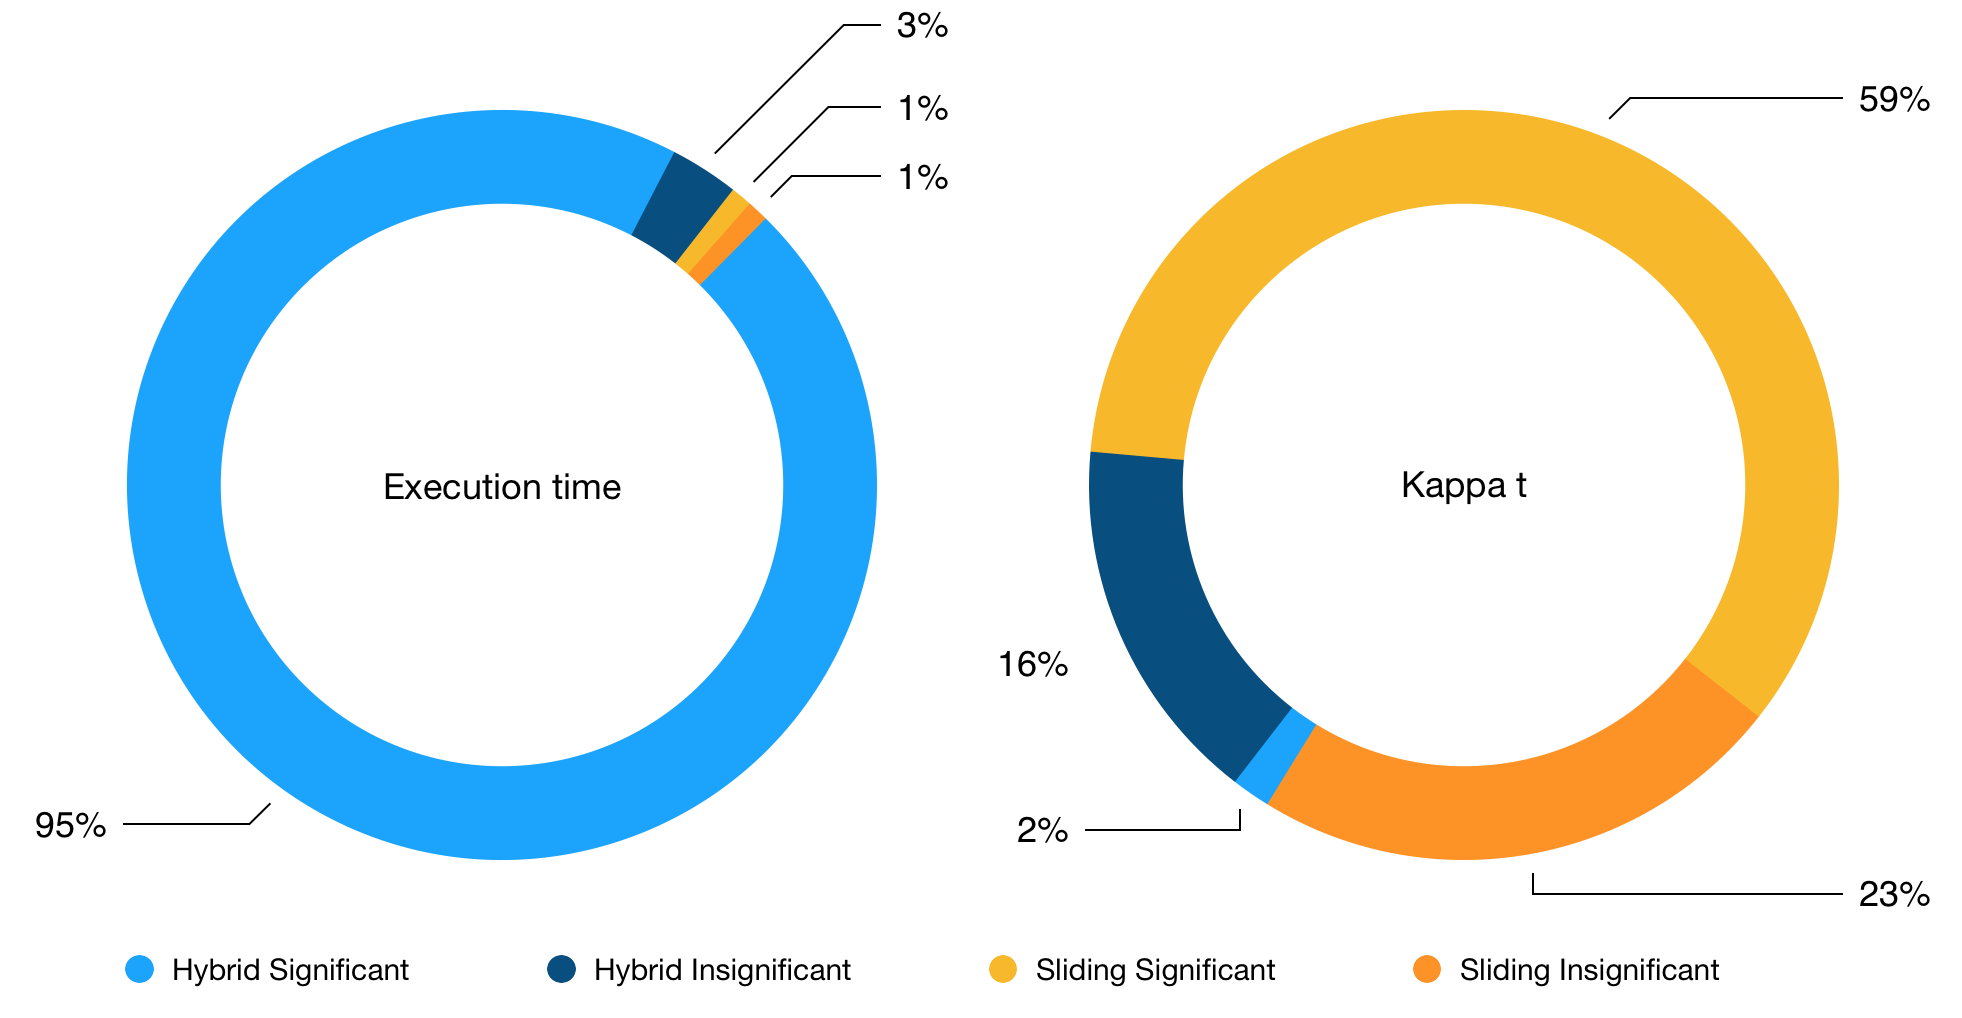
\includegraphics[width=\linewidth]{./images/wilcoxon_window_type_pie}
\caption{\label{fig:wilcoxon_window_type_pie}Pie chart illustrating table \ref{table:wilcoxon_window_type}}
\end{figure}


When we dig deeper into the \textit{Window Type} parameter, as we can see from table \ref{table:wilcoxon_window_type}  and figure \ref{fig:wilcoxon_window_type_pie}, for the execution time metric, \textit{hybrid} is evidently the best choice as it ranks best across 98\% of parameter combinations. For the $\kappa_t$ metric, it is just as obvious as \textit{sliding} ranks best across about 82\% of the parameter combinations. 

The \textit{Window Type} parameter ranking results suggest that \textit{hybrid windowing} has a significant impact on the execution time of the algorithm, independently of other parameters values. This suggests that choosing the \textit{hybrid windowing} value for the \textit{Window Type} parameter could be very beneficial in reducing the execution time of the algorithm. Again, this is exactly as expected: the implementation of \textit{hybrid windowing} is such that each sub-classifier in the ensemble only trains on each instance once, whereas the \textit{sliding windowing} technique is implemented such that each sub-classifier in the ensemble trains on each instance at least once. This, logically, leads to fewer operations, and therefore a reduction in execution time for the algorithm. This should hold true across all data streams, and therefore we recommend anyone who chooses to run this algorithm with the intent of reducing the execution time to choose the \textit{hybrid windowing} parameter value.
However, we also found that \textit{sliding windowing} outperforms \textit{hybrid windowing} across most parameter combinations, with or without a significant statistical difference. Again, using the explanation above for the reduction in execution time, since each sub-classifier training using \textit{sliding windowing} trains on each instance multiple times, it is logical that it is better able to fit the data instance in its model. 
This means that the algorithm presents a trade-off between execution time and predictive accuracy when considering the \textit{Window Type} parameter. Whoever runs the algorithm must choose which metric they value more, and choose a windowing type accordingly.

As other parameters can take more than two values, we must use the Friedman test in combination with the post-hoc Nemenyi test in order to test our null hypotheses.

\subsection{Post-hoc Nemenyi tests}

\begin{table}[]
\centering
\caption{\label{table:nemenyi_significant_breakdown}Percentage of parameter combinations that showed statistically significant differences from the post-hoc Nemenyi test}
\begin{tabular}{|l|l|c|l|c|l|}
\hline
\textbf{Parameter} & \textbf{Measure} & \textbf{Significant} & \textbf{\%} & \textbf{Insignificant} & \textbf{\%} \\ \hline \hhline{======}
\multirow{2}{*}{Batch size} & $\kappa_t$ & $\frac{1}{330}$ & $0.3\%$ & $\frac{229}{330}$ & $99.70\%$ \\ \cline{2-6} 
 & execution time & $\frac{287}{330}$ & $86.97\%$ & $\frac{43}{330}$ & $13.03\%$ \\ \hline \hhline{======}
\multirow{2}{*}{Drift reset type} & $\kappa_t$ & $\frac{1}{330}$ & $0.30\%$ & $\frac{329}{330}$ & $99.70\%$ \\ \cline{2-6} 
 & execution time & $\frac{64}{330}$ & $19.39\%$ & $\frac{266}{330}$ & $80.61\%$ \\ \hline \hhline{======}
\multirow{2}{*}{Ground truth} & $\kappa_t$ & $\frac{57}{198}$ & $28.79\%$ & $\frac{141}{198}$ & $71.21\%$ \\ \cline{2-6} 
 & execution time & $\frac{168}{198}$ & $84.85\%$ & $\frac{30}{198}$ & $15.15\%$ \\ \hline \hhline{======}
\multirow{2}{*}{Voting type} & $\kappa_t$ & $\frac{0}{180}$ & $0\%$ & $\frac{180}{180}$ & $100.00\%$ \\ \cline{2-6} 
 & execution time & $\frac{154}{180}$ & $85.56\%$ & $\frac{26}{180}$ & $14.44\%$ \\ \hline
\end{tabular}
\end{table}

\begin{table}[]
\centering
\caption{\label{table:nemenyi_significant_breakdown_aggregate}Number of different ranking and statistically significant parameter combinations from table \ref{table:nemenyi_significant_breakdown}}
\begin{tabular}{|l|l|c|c|}
\hline
\textbf{Parameter} & \textbf{Measure} & \textbf{Significant} & \textbf{Insignificant} \\ \hline \hhline{====}
\multirow{2}{*}{Batch size} & $\kappa_t$ & $ 1 \rightarrow 1 $ & $ 229 \rightarrow 6 $ \\ \cline{2-4} 
 & execution time & $ 287 \rightarrow 2 $ & $ 43 \rightarrow 2 $ \\ \hline \hhline{====}
\multirow{2}{*}{Drift reset type} & $\kappa_t$ & $ 1 \rightarrow 1 $ & $ 229 \rightarrow 6 $ \\ \cline{2-4} 
 & execution time & $ 64 \rightarrow 6 $ & $ 266 \rightarrow 6 $ \\ \hline \hhline{====}
\multirow{2}{*}{Ground truth} & $\kappa_t$ & $ 57 \rightarrow 3 $ & $ 141 \rightarrow 6 $ \\ \cline{2-4} 
 & execution time & $ 168 \rightarrow 22 $ & $ 30 \rightarrow 16 $ \\ \hline \hhline{====}
\multirow{2}{*}{Voting type} & $\kappa_t$ & $ 0 \rightarrow 0 $ & $ 180 \rightarrow 4 $ \\ \cline{2-4} 
 & execution time & $ 154 \rightarrow 2 $ & $ 26 \rightarrow 3 $ \\ \hline
\end{tabular}
\end{table}

\subsubsection{Batch Size}

As we can see from table \ref{table:nemenyi_significant_breakdown}, only 1 combination of parameters among 330 were significantly statistically different when considering the $\kappa_t$ metric for the batch size parameter, which is a negligible amount. As for the execution time metric, we can see that almost $87\%$ of parameter combinations proved to show a significant statistical difference. This confirms our expectations that changing only the batch size has a large impact on the execution time of the algorithm but no significant impact on its predictive accuracy.
The first row of table \ref{table:nemenyi_significant_breakdown_aggregate} indicates that there are 7 variations of rankings of batch size rankings for the $\kappa_t$ metric; the second line indicates that there are 2 variations of rankings and pairs of parameters that were significantly statistically different and 2 variations of ranks for batch sizes that were insignificant. These values are seen in table \ref{table:batch_size_rankings} and figure \ref{fig:batch_size_rankings_pie}.

\begin{table}[]
\centering
\caption{\label{table:batch_size_rankings}Rankings for batch size and parameter combination counts}
\begin{tabular}{|l|c|l|c|c|}
\hline
\textbf{Metric} & \textbf{Stat. Sig.} & \textbf{Ranks} & \textbf{Stat. Sig. values} & \textbf{\%} \\ \hline \hhline{=====}
\multirow{7}{*}{$\kappa_t$} & \checkmark & 25 / 75 / 100 & 25 / 100 & 0.30\% \\ \cline{2-5} 
 & \multirow{6}{*}{$\times$} & 100 / 25 / 75 & \multirow{6}{*}{} & 16.36\% \\ \cline{3-3} \cline{5-5} 
 &  & 100 / 75 / 25 &  & 10.30\% \\ \cline{3-3} \cline{5-5} 
 &  & 25 / 100 / 75 &  & 16.67\% \\ \cline{3-3} \cline{5-5} 
 &  & 25 / 75 / 100 &  & 27.58\% \\ \cline{3-3} \cline{5-5} 
 &  & 75 / 100 / 25 &  & 10.00\% \\ \cline{3-3} \cline{5-5} 
 &  & 75 / 25 / 100 &  & 18.79\% \\ \hline \hhline{=====}
\multirow{4}{*}{Execution time} & \multirow{2}{*}{\checkmark} & 100 / 75 / 25 & 100 / 25 & 71.52\% \\ \cline{3-5} 
 &  & 75 / 100 / 25 & 75 / 25 & 15.45\% \\ \cline{2-5} 
 & \multirow{2}{*}{$\times$} & 100 / 75 / 25 & \multirow{2}{*}{} & 6.67\% \\ \cline{3-3} \cline{5-5} 
 &  & 75 / 100 / 25 &  & 6.36\% \\ \hline
\end{tabular}
\end{table}

\begin{figure}
  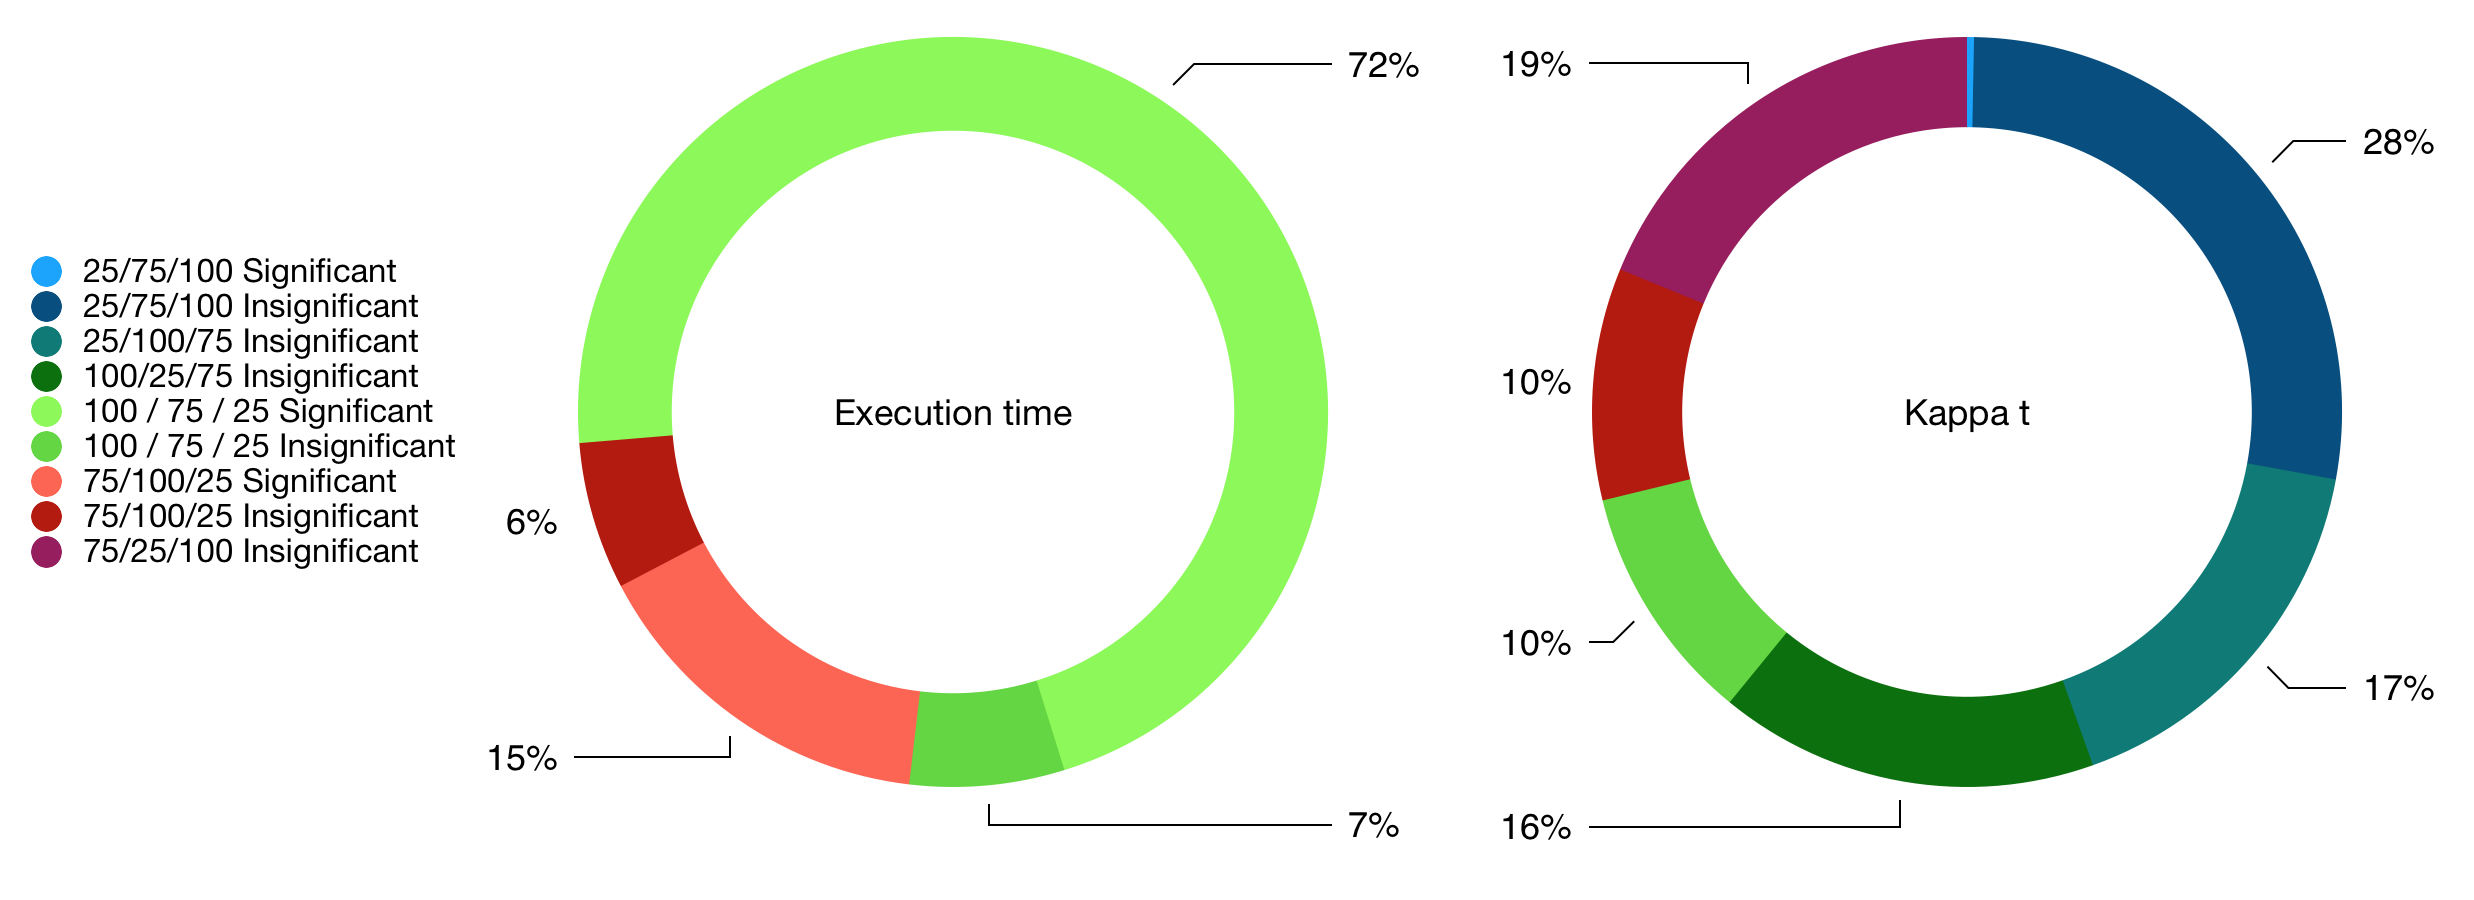
\includegraphics[width=\linewidth]{./images/batch_size_rankings_pie}
\caption{\label{fig:batch_size_rankings_pie}Pie chart illustrating table \ref{table:batch_size_rankings}}
\end{figure}

Let us examine the pie charts illustrating the rankings of the \textit{Batch size} parameter values.
We will first examine the results for the execution time. At first glance, we notice that \textit{100} clearly ranks first over the majority of parameter combinations, followed by \textit{75} over a minority of combinations.
For the $\kappa_t$ metric, the rankings are less clear. \textit{25} seems to rank first more frequently (across $45\%$ of parameter combinations), whereas \textit{75} and \textit{100} rank first across $26\%$ of parameter combinations each. These rankings do not tell us how much the difference is across parameter combinations. By this, we mean that while a parameter value may rank first across a larger percentage of parameter combinations, it may actually perform worse than another value over a smaller percentage of parameter combinations.
In any case, the results indicate that there is another trade-off to be made in regards to the batch size parameter between predictive accuracy and execution time. Again, we expected these results as a batch size of 100 allows the ensemble to learn from more examples at once, which reduces the quantity of operations that would have to be repeated were we to use a batch size of 25 for example, where each operation down the line would be run 4 times instead of only 1 time. As for predictive accuracy, \textit{25} has a slight advantage over the other parameter values possibly because there is a better chance that a drift wreaks havoc on a sub-classifier's ability to train on a batch of \textit{75} or \textit{100} than on a batch of \textit{25}. For a batch of \textit{25}, the sub-classifiers can be reset sooner, and the next batch may be easier to model.

\subsubsection{Drift Reset Type}

Let us now investigate the Drift Reset Type parameter. As we can see from table \ref{table:nemenyi_significant_breakdown}, only a single out of 330 parameter combinations showed a significant statistical difference in parameter values when considering the $\kappa_t$ metric, whereas about $20\%$ of parameter values showed a statistical significant difference in parameter values when considering the execution time metric. This suggests that the value of the drift reset type parameter does not have a significant impact over other values on the measured metrics.
Table \ref{table:nemenyi_significant_breakdown_aggregate}, lists the number of different rankings found in table \ref{table:drift_reset_type_rankings} over the measured metrics, depending on whether results showed a statistical significant difference.

Let us examine table \ref{table:drift_reset_type_rankings} or better yet, the pie charts seen in figure \ref{drift_reset_type_rankings_pie} illustrating the rankings of the \textit{Drift Reset Type} parameter values.
Again, we will first examine the results for the execution time. At first glance, we notice that \textit{blind resets} clearly ranks first the least over the parameter combinations. \textit{Reset all} ranks first across half of the parameter combinations and \textit{partial resets} over about a third of them. This is a good sign, and expected. Since sub-classifiers must be reset more frequently, they must be completely re-trained on data, which also prevents them from learning from a larger set of older data. This might be good for streams with very frequent drifts, but those where they appear infrequently, blindly resetting the classifier prevents it from remembering possibly useful historical data.

For the $\kappa_t$ metric, the rankings are not as clear. Again, we must remember that these rankings do not tell us the difference across parameter combinations, meaning that while a parameter value may rank first across a larger percentage of parameter combinations, it may perform less well than another value over a smaller percentage of parameter combinations.
In any case, the results indicate that each parameter value ranks first across a third of parameter combinations. This does not allow us to conclude much, other than blind resets may perform just as well as resetting every sub-classifier or only a minority of them. It could be that the sub-classifiers are not very apt at learning from the data, or that resetting the sub-classifiers is not very effective. Another reason could be attributed to the way partial drift resets work, in that each sub-classifier has a chance of being reset, meaning that there is a chance that the offending sub-classifier that is not properly adapting to the concept drift is not reset. A more thorough investigation is unfortunately outside of the scope of this work, due to time constraints. It could also be that the predictive accuracy can not improve much after a drift due to the limitations of the sub-classifiers to model the data effectively. Either way, this is truly unfortunate, as it suggests that changing how often and how many sub-classifiers are reset does not seem to affect the $\kappa_t$ metric.
These results indicate that blind resets perform almost as well as our other reset strategies, which may suggest that our drift reset strategy needs further investigation.

\begin{table}[]
\centering
\caption{\label{table:drift_reset_type_rankings}Rankings for drift reset type and parameter combination counts}
\begin{tabular}{|l|c|l|c|c|}
\hline
\textbf{Metric} & \textbf{Stat. Sig.} & \textbf{Ranks} & \textbf{Stat. Sig. values} & \textbf{\%} \\ \hline \hhline{=====}
\multirow{7}{*}{$\kappa_t$} & \checkmark & BLIND / ALL / PARTIAL & BLIND / PARTIAL & 0.30\% \\ \cline{2-5}
 & \multirow{6}{*}{$\times$} & ALL / BLIND / PARTIAL & \multirow{6}{*}{} & 23.64\% \\ \cline{3-3} \cline{5-5} 
 &  & ALL / PARTIAL / BLIND &  & 13.64\% \\ \cline{3-3} \cline{5-5} 
 &  & BLIND / ALL / PARTIAL &  & 15.45\% \\ \cline{3-3} \cline{5-5} 
 &  & BLIND / PARTIAL / ALL &  & 17.88\% \\ \cline{3-3} \cline{5-5} 
 &  & PARTIAL / ALL / BLIND &  & 14.24\% \\ \cline{3-3} \cline{5-5} 
 &  & PARTIAL / BLIND / ALL &  & 14.85\% \\ \hline \hhline{=====}
\multirow{12}{2cm}{Execution time} & \multirow{6}{*}{\checkmark} & ALL / PARTIAL / BLIND & ALL / BLIND & 6.97\% \\ \cline{3-5} 
 &  & ALL / BLIND / PARTIAL & ALL / PARTIAL & 0.61\% \\ \cline{3-5} 
 &  & BLIND / PARTIAL / ALL & BLIND / ALL & 0.91\% \\ \cline{3-5} 
 &  & BLIND / ALL / PARTIAL & BLIND / PARTIAL & 0.91\% \\ \cline{3-5} 
 &  & PARTIAL / BLIND / ALL & PARTIAL / ALL & 1.52\% \\ \cline{3-5} 
 &  & PARTIAL / ALL / BLIND & PARTIAL / BLIND & 8.48\% \\ \cline{2-5} 
 & \multirow{6}{*}{$\times$} & ALL / BLIND / PARTIAL & \multirow{6}{*}{} & 6.36\% \\ \cline{3-3} \cline{5-5} 
 &  & ALL / PARTIAL / BLIND &  & 36.36\% \\ \cline{3-3} \cline{5-5} 
 &  & BLIND / ALL / PARTIAL &  & 7.58\% \\ \cline{3-3} \cline{5-5} 
 &  & BLIND / PARTIAL / ALL &  & 5.45\% \\ \cline{3-3} \cline{5-5} 
 &  & PARTIAL / ALL / BLIND &  & 21.82\% \\ \cline{3-3} \cline{5-5} 
 &  & PARTIAL / BLIND / ALL &  & 3.03\% \\ \hline
\end{tabular}
\end{table}

\begin{figure}
  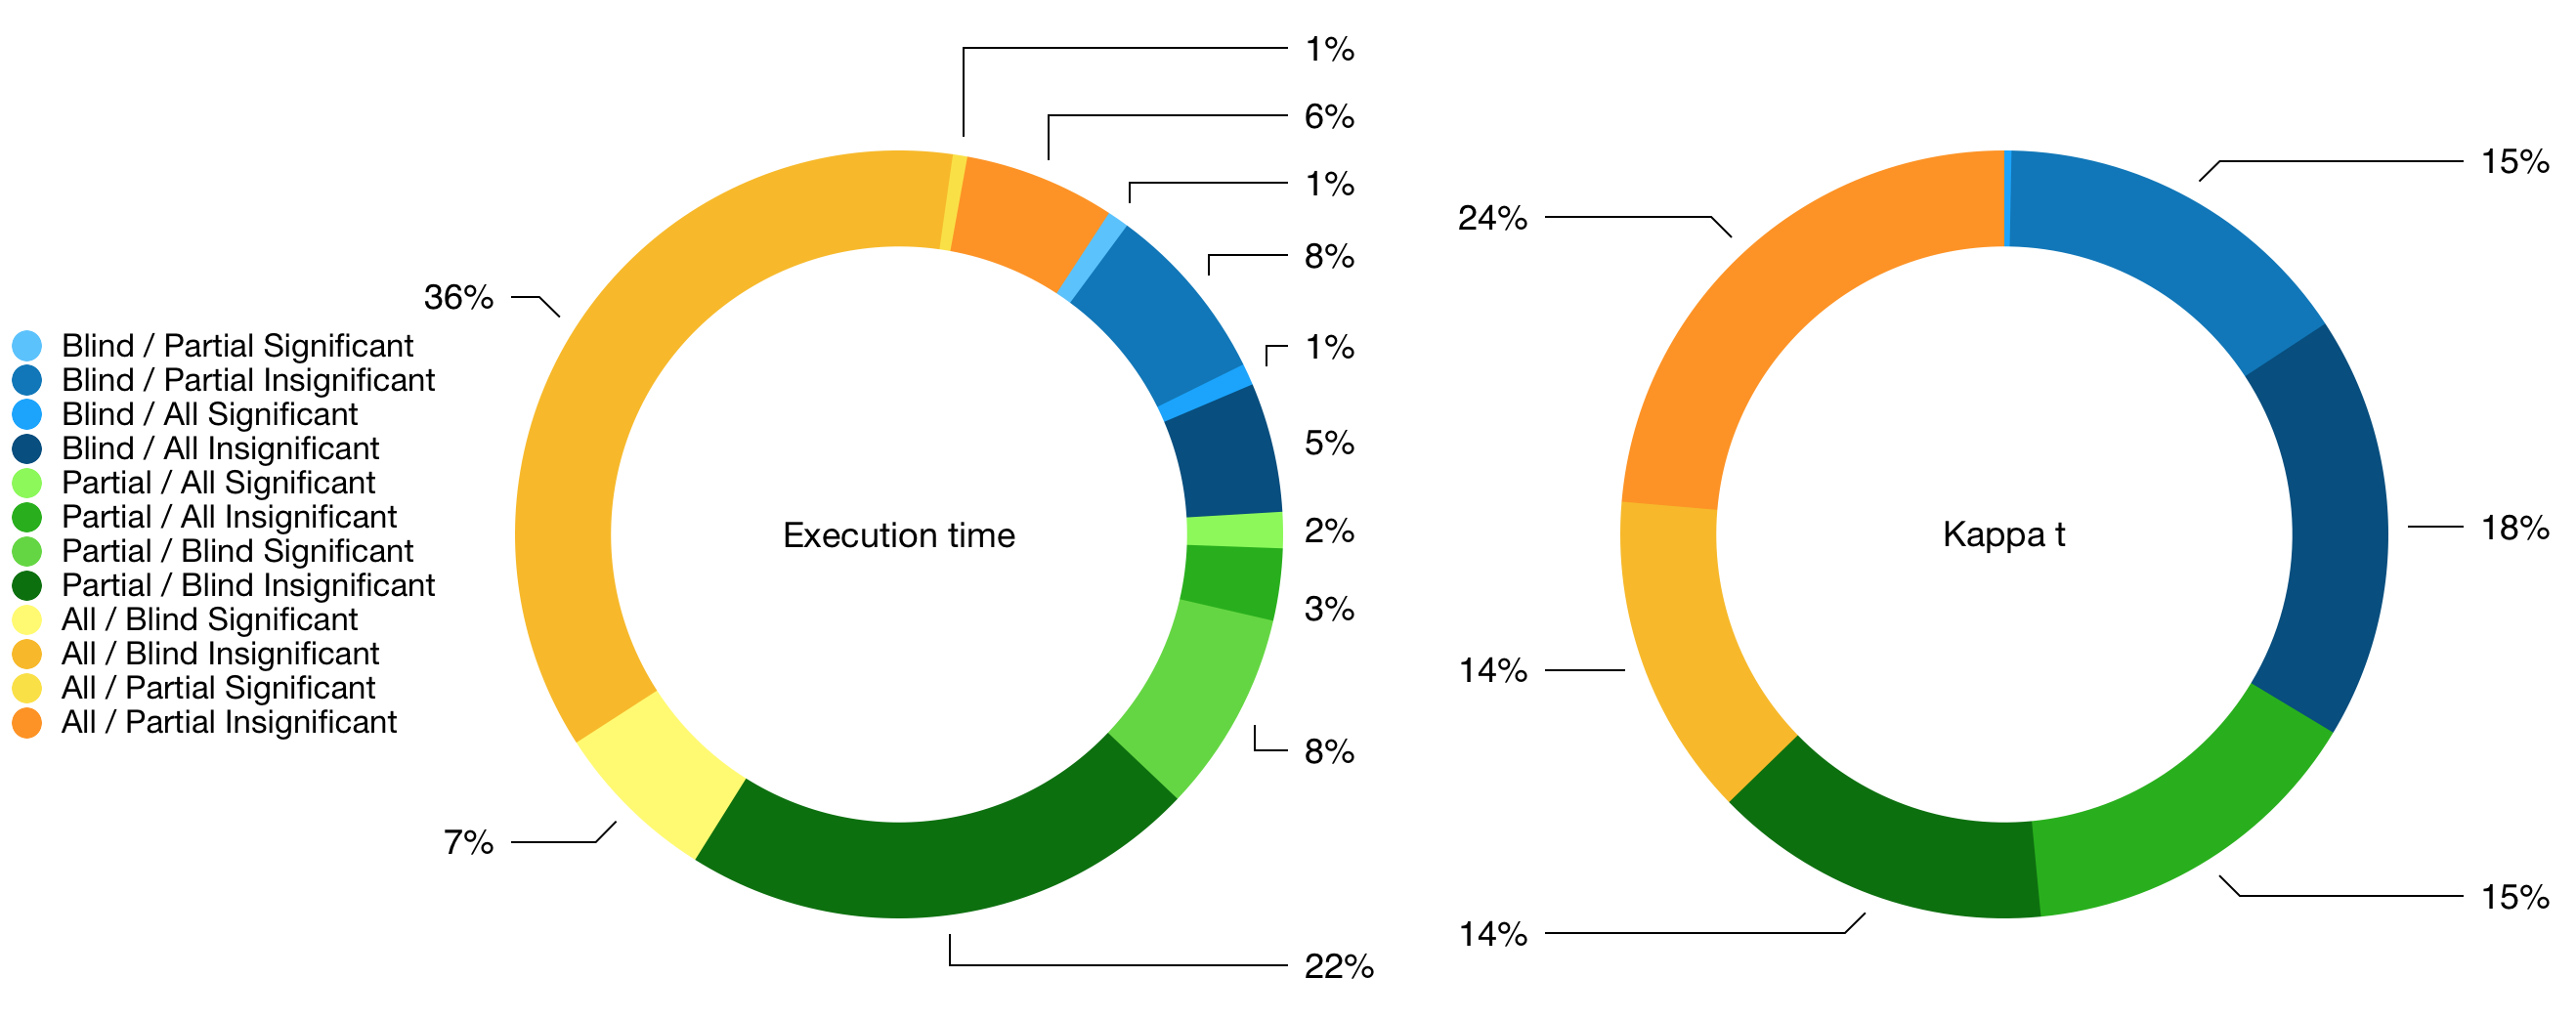
\includegraphics[width=\linewidth]{./images/drift_reset_type_rankings_pie}
\caption{\label{fig:drift_reset_type_rankings_pie}Pie chart illustrating table \ref{table:drift_reset_type_rankings}}
\end{figure}

\subsubsection{Ground Truth}

Let us now investigate the Ground Truth parameter (\textbf{which indicates the percentage of labelled instances used to train our ensemble}). Table \ref{table:nemenyi_significant_breakdown} shows that less than one third of parameter combinations show a statistical significance difference for the $\kappa_t$ metric; but over $84\%$ for the execution time metric. This suggests that the value of the ground truth parameter has a measurable impact on the execution time, across a large portion of the other parameters, (almost) no matter their values.

Table \ref{table:ground_truth_rankings} \textbf{shows that}, for the $\kappa_t$ metric, there are multiple possible options for ranking the parameter values. For those with a statistical significant difference, 100 performs better than 60. 100 ranks first across all parameter combinations over $98\%$ of the time, as expected. This is normal, as we expect our ensemble to better learn to model the streamed data from ground truth rather than from its own predictions of class label values, considering that it can enable our ensemble to learn from erroneously labelled data. It is a good sign, however, that there is no statistical significant difference for parameter values other than 100 and 60. It is logical that selecting a higher percentage of ground truth will lead to higher predictive accuracy, but we can allow for a trade-off between predictive accuracy and time.

\textbf{We can also see}, from table \ref{table:ground_truth_rankings}, that there are a lot of different combinations for ranks and statistical significant different values for the execution time metric. $60\%$ ground truth ranks first across $74.31\%$ of parameter combinations, and $100\%$ ground truth ranks first across only $17.71\%$ of parameter values. When we exclude insignificant results, our previous observation remains true, but across a smaller percentage of parameter combinations, but only by $5\%$ to $10\%$. We can conclude that the using $60\%$ ground truth is more likely to decrease execution time. This is an unexpected finding, as we expected that using less ground truth would cause an increase in execution time by causing more drift detection events and therefore more model resets and retrains. However, it is possible that by using less ground truth, there are no drift detection events because the model is not able to properly learn from the data, so the model is never reset or retrained which might also explain why this parameter value also ranks as one of the worst in predictive accuracy.

When looking at the raw values, as \textbf{depicted} in figure \ref{fig:order_by_ground_truth}, we notice that the $\kappa_t$ metric does not change much over the parameter combinations, but rises noticeably starting when using $80\%$ ground truth. The regular peaks and valleys within each set of ground truth values (separated by black vertical lines) simply represent how other parameters affect $\kappa_t$. We also notice that the amount of ground truth has a strong effect over the sine1, mixed and particularly on the circles data sets. It may be that it is easier to model the data from SEA than from the other data sets, and therefore it does not need as much ground truth to build an accurate model. Not much can be said when looking at the raw values for the execution time metric other than that there may be fewer valleys in the section dedicated for the $60\%$ ground truth parameter.

\begin{table}[]
\centering
\caption{\label{table:ground_truth_rankings}Rankings for ground truth and parameter combination counts}
\begin{tabular}{|l|c|l|c|c|}
\hline
\textbf{Metric} & \textbf{Stat. Sig.} & \textbf{Ranks} & \textbf{Stat. Sig. values} & \textbf{\%} \\ \hline
\multirow{4}{*}{$\kappa_t$} & \checkmark & 100 / x / x / x / 60 & 100 / 60 & 28.80\% \\ \cline{2-5} 
 & \multirow{3}{*}{$\times$} & 100 / x / x / x / 60 & \multirow{3}{*}{} & 65.15\% \\ \cline{3-3} \cline{5-5} 
 &  & 100 / x / x / 60 / 70 &  & 4.55\% \\ \cline{3-3} \cline{5-5} 
 &  & 80 / 100 / 90 / 70 / 60 &  & 1.52\% \\ \hline
\multirow{21}{*}{Execution time} & \multirow{12}{*}{\checkmark} & 100 / 60 / x / x / 70 & 100 / 70 & 9.10\% \\ \cline{3-5} 
 &  & 100 / 60 / 90 / 80 / 70 & \begin{tabular}[c]{@{}c@{}}100 / 70\\ 60 / 70\end{tabular} & 0.51\% \\ \cline{3-5} 
 &  & 100 / 60 / 90 / 70 / 80 & 100 / 80 & 2.02\% \\ \cline{3-5} 
 &  & 100 / 60 / 80 / 70 / 90 & 100 / 90 & 0.51\% \\ \cline{3-5} 
 &  & 60 / x / x / x / 100 & 60 / 100 & 14.16\% \\ \cline{3-5} 
 &  & 60 / x / x / x / 70 & 60 / 70 & 1.02\% \\ \cline{3-5} 
 &  & 60 / x / x / x / 80 & 60 / 80 & 50.51\% \\ \cline{3-5} 
 &  & 60 / 70 / 100 / 80 / 90 & \begin{tabular}[c]{@{}c@{}}60 / 80\\ 60 / 90\end{tabular} & 0.51\% \\ \cline{3-5} 
 &  & 60 / 80 / 70 / 100 / 90 & 60 / 90 & 1.01\% \\ \cline{3-5} 
 &  & 70 / 90 / 80 / 100 / 60 & \begin{tabular}[c]{@{}c@{}}70 / 60\\ 90 / 60\end{tabular} & 0.51\% \\ \cline{3-5} 
 &  & 90 / x / x / x / 100 & 90 / 100 & 2.03\% \\ \cline{3-5} 
 &  & 90 / 70 / 80 / 100 / 60 & 90 / 60 & 3.03\% \\ \cline{2-5} 
 & \multirow{9}{*}{$\times$} & 100 / 60 / x / x / 90 & \multirow{9}{*}{} & 1.02\% \\ \cline{3-3} \cline{5-5} 
 &  & 100 / 60 / x / x / 70 &  & 1.52\% \\ \cline{3-3} \cline{5-5} 
 &  & 100 / 60 / 90 / 70 / 80 &  & 3.03\% \\ \cline{3-3} \cline{5-5} 
 &  & 60 / x / x / 80 / 90 &  & 1.52\% \\ \cline{3-3} \cline{5-5} 
 &  & 60 / x / x / x / 80 &  & 3.55\% \\ \cline{3-3} \cline{5-5} 
 &  & 60 / 100 / 90 / 80 / 70 &  & 0.51\% \\ \cline{3-3} \cline{5-5} 
 &  & 60 / x / x / 80 / 100 &  & 1.52\% \\ \cline{3-3} \cline{5-5} 
 &  & 90 / x / x / x / 100 &  & 2.03\% \\ \cline{3-3} \cline{5-5} 
 &  & 90 / 70 / 80 / 100 / 60 &  & 0.51\% \\ \hline
\end{tabular}
\end{table}

\begin{figure}
  \includegraphics[width=\linewidth]{./images/ground_truth}
\caption{\label{fig:order_by_ground_truth}$\kappa_t$ across all parameter combinations, ordered by ground truth}
\end{figure}

\subsubsection{Voting Type}

And finally, we will investigate the Voting Type parameter. As we can see from table \ref{table:nemenyi_significant_breakdown}, none of the 180 parameter combinations proved to show a significant statistical difference for the $\kappa_t$ metric. However, a large portion of the parameter combinations showed a significant statistical significance for the execution time parameter ($85.56\%$ of combinations). This leads us to believe that the voting type does not have a major influence on the prediction accuracy. However, for execution time, there is a statistical significant difference present across a good majority of parameter combinations, leading us to believe that the significance remains true across a good portion of other parameter values.

As we can see from table \ref{table:nemenyi_significant_breakdown_aggregate}, there are not very many different possible rankings for both metrics. Indeed, there are 4 possible rankings for $\kappa_t$ and 5 for the execution time metric.

Let us now examine table \ref{table:voting_type_rankings}, or better yet the pie charts from figure \ref{fig:voting_type_rankings_pie} for the \textit{Voting Type} parameter.
We will first examine the results for the execution time. At first glance, it is clear that \textit{probability voting} ranks first amongst the majority of parameter combinations ($90\%$ of them), while \textit{weighted averaged probability voting} ranks first amongst the remaining $10\%$ of parameter combinations. We can say with the utmost certainty that \textit{averaged weighted probability voting} is not a good choice for a parameter value if the goal is to keep execution time low, as it ranks last over $99\%$ of parameter combinations. It makes sense that probability voting ranks first in execution time over most parameter combinations as its implementation is such that the two other voting schemes add to the operations computed for probability voting. In other words, for the other two voting schemes, the results obtained through probability voting is an intermediate result.

For the $\kappa_t$ metric, \textit{probability voting} ranks first across about $69\%$ of parameter combinations, and \textit{weighted averaged probability voting} ranking first across the remaining fraction of parameter combinations. Probability voting appears to rank better than the other two voting schemes, but this could be due to the noise that we add when we apply the weights to the prediction probabilities. Furthermore, the ranks do not allow us to determine by how much the voting scheme impacts the actual metrics. Then, to answer why \textit{weighted averaged probability voting} performs better than \textit{averaged weighted probability voting}, it could be that there is less noise introduced by first averaging the prediction probabilities then applying the weight, than doing those operations in the opposite way.

When we look at the raw results from our simulations, and order them by voting type (then by ground truth), as seen in figure \ref{fig:order_by_voting_type}, we can notice that there is no significant difference in the $\kappa_t$ values between probability voting and weighted averaged probability voting. However, we can see a significant difference between probability voting and averaged weighted probability voting.

The best choice here appears to be \textit{probability voting}, but we will be able to better determine the veracity of this statement when ranking all parameter combinations and comparing their raw metric values in the next section. It does not matter whether execution time or predictive accuracy matters more, probability voting is more likely to better model the data, predict new instances all the while taking the least amount of time to do so, as opposed to the other parameter values.

\begin{table}[]
\centering
\caption{\label{table:voting_type_rankings}Rankings for voting type and parameter combination counts}
\begin{tabular}{|l|c|l|c|c|}
\hline
\textbf{Metric} & \textbf{Stat. Sig.} & \textbf{Ranks} & \textbf{Stat. Sig. values} & \textbf{\%} \\ \hline \hhline{=====}
\multirow{4}{*}{$\kappa_t$} & \multirow{4}{*}{$\times$} & PROBA / AVG W / W AVG & \multirow{4}{*}{} & 1.11\% \\ \cline{3-3} \cline{5-5} 
 &  & PROBA / W AVG / AVG W &  & 67.78\% \\ \cline{3-3} \cline{5-5} 
 &  & W AVG / AVG W / PROBA &  & 1.11\% \\ \cline{3-3} \cline{5-5} 
 &  & W AVG / PROBA / AVG W &  & 30.00\% \\ \hline \hhline{=====}
\multirow{5}{2cm}{Execution time} & \multirow{2}{*}{\checkmark} & PROBA / W AVG / AVG W & PROBA / AVG W & 78.33\% \\ \cline{3-5} 
 &  & W AVG / PROBA / AVG W & W AVG / AVG W & 7.22\% \\ \cline{2-5} 
 & \multirow{3}{*}{$\times$} & PROBA / AVG W / W AVG & \multirow{3}{*}{} & 0.56\% \\ \cline{3-3} \cline{5-5} 
 &  & PROBA / W AVG / AVG W &  & 11.11\% \\ \cline{3-3} \cline{5-5} 
 &  & W AVG / PROBA / AVG W &  & 2.78\% \\ \hline
\end{tabular}
\end{table}

\begin{figure}
  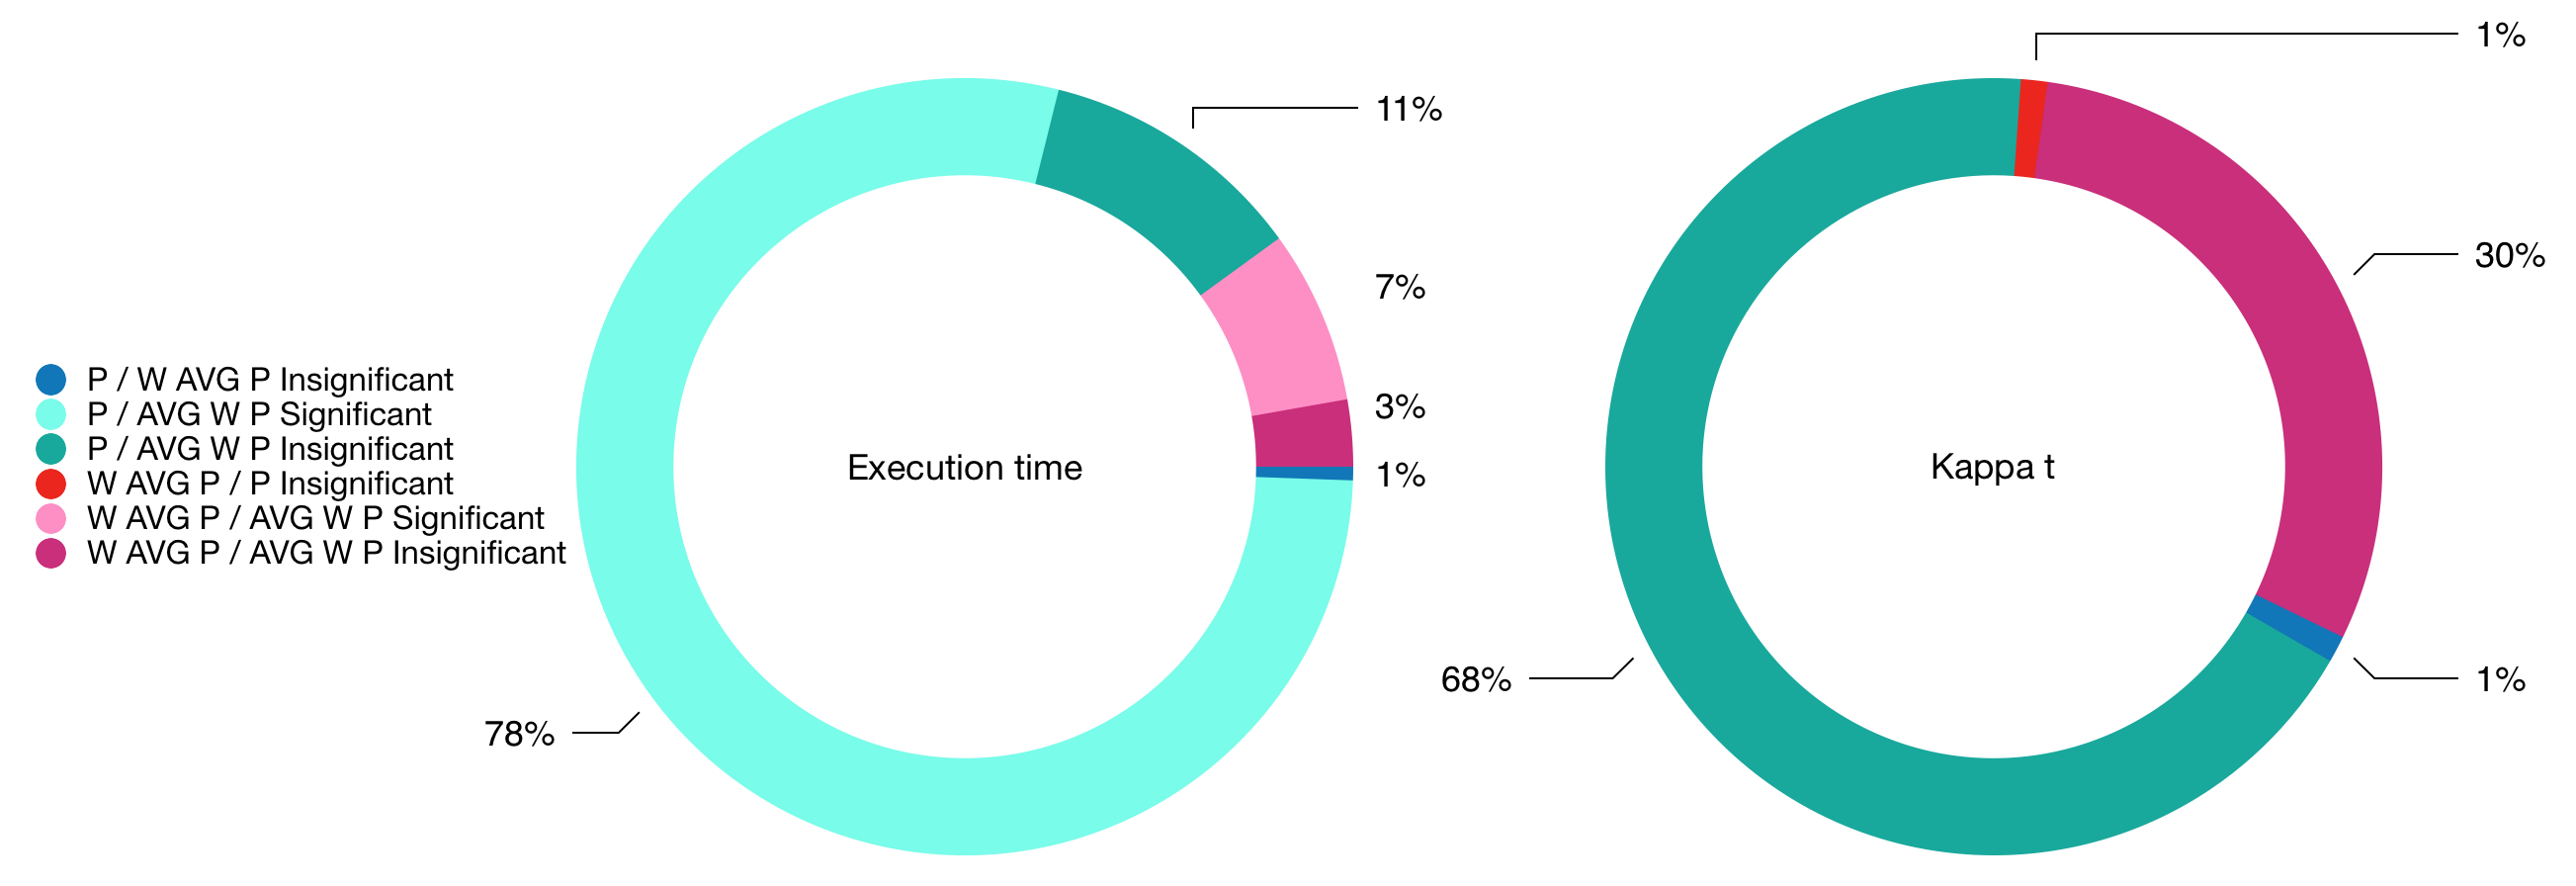
\includegraphics[width=\linewidth]{./images/voting_type_rankings_pie}
\caption{\label{fig:voting_type_rankings_pie}Pie chart \textbf{illustrating} table \ref{table:voting_type_rankings}}
\end{figure}

\begin{figure}
  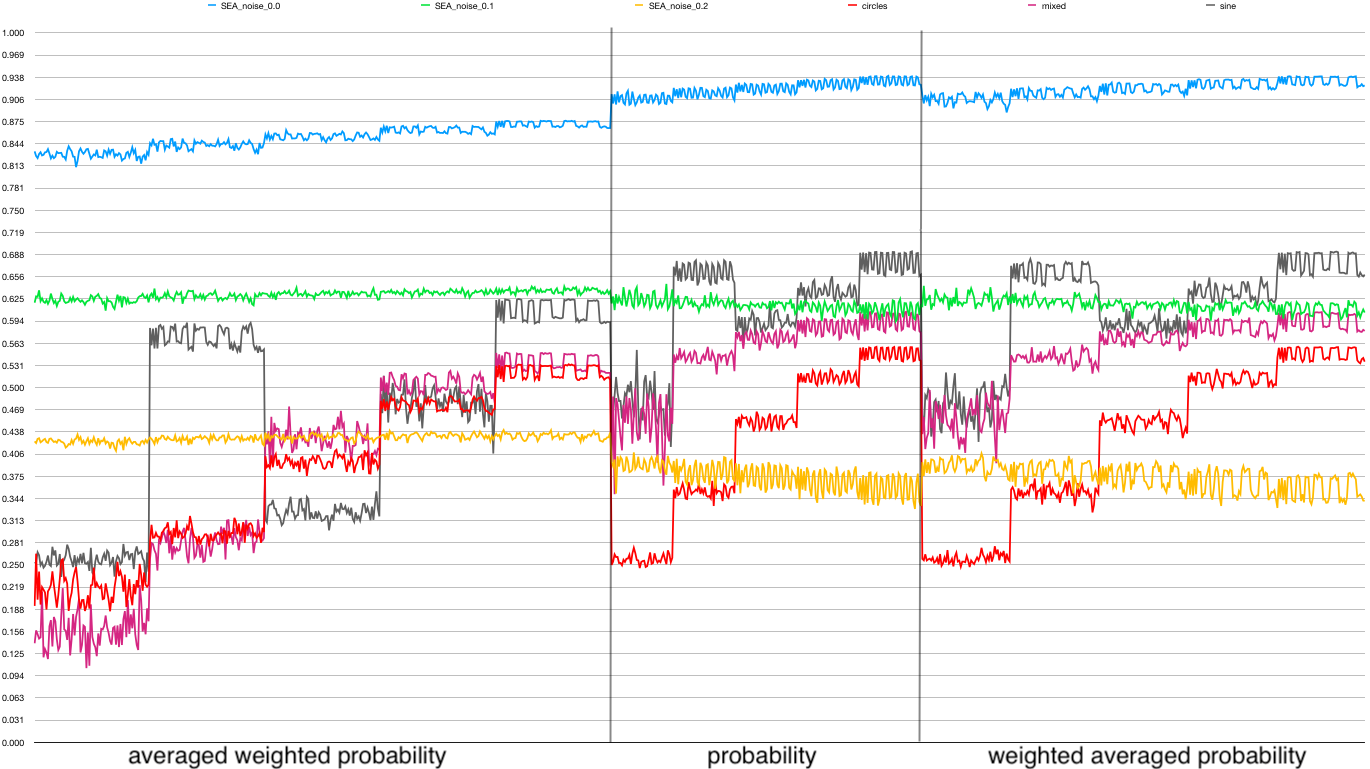
\includegraphics[width=\linewidth]{./images/raw_voting_type}
\caption{\label{fig:order_by_voting_type}$\kappa_t$ across all parameter combinations, ordered by voting type}
\end{figure}

\subsection{Summary}
The above results suggest that it is preferable to use the following parameter combination to obtain higher $\kappa_t$ values: [\textit{sliding, probability, 25, $100\%$, all, 1e}].
\textbf{Otherwise,} to minimise the execution time, the results suggest to use [\textit{hybrid, probability, 100, $60\%$, all, 1e / 1c}].

The differences lie with the window type, the batch size, the ground truth used and partially the drift detector count. The results above indicated that using probability voting,  1 detector per ensemble to detect drifts, and resetting all classifiers when drifts occur would lead to better $\kappa_t$ values and a lower execution time. For the batch size, window type, and the drift detector count, it is completely logical that choosing one value over another would change the execution time as they were, at least partially, implemented as time saving measures.

In the following section, we will rank the parameter combinations to determine if the ones listed two paragraphs above are truly top ranking.

\section{Comparing all parameter combinations}
In this section, we aim to rank all 1110 parameter combinations \textbf{to determine which parameters perform the best, and those that perform the worst}. This will be done in three different configurations:
\begin{enumerate}
\item over $\kappa_t$
\item over execution time
\item over both metrics
\end{enumerate}

For figures \ref{fig:rank_kappa} and \ref{fig:rank_seconds}, the parameter values are shortened to improve readability.
The values are split by vertical lines. See table \ref{table:ranking_parameter_values_mapping} for the mapping between shortened and real parameter values. The order of the parameters in the figures are the following: [\textit{window type, voting type, ground truth, batch size, drift reset type, detector count, detector content}].

\begin{table}[]
\centering
\caption{\label{table:ranking_parameter_values_mapping}Mapping shortened parameter values with full name}
\begin{tabular}{|l|c|l|}
\hline
\textbf{Parameter} & \textbf{Value} & \textbf{Real Value} \\ \hline
\multirow{2}{*}{Window type} & s & Sliding \\ \cline{2-3} 
 & h & Hybrid \\ \hline
\multirow{4}{*}{Voting type} & aw & Averaged weighted probability \\ \cline{2-3} 
 & b & Boolean \\ \cline{2-3} 
 & p & Probability \\ \cline{2-3} 
 & wa & Weighted averaged probability \\ \hline
\multirow{4}{*}{Drift reset type} & a & All \\ \cline{2-3} 
 & b & Blind \\ \cline{2-3} 
 & n & None \\ \cline{2-3} 
 & p & Partial \\ \hline
\multirow{2}{*}{Detector count} & 1c & 1 per classifier \\ \cline{2-3} 
 & 1e & 1 for ensemble \\ \hline
\multirow{3}{*}{Detector content} & b & Boolean \\ \cline{2-3} 
 & p & Probability \\ \cline{2-3} 
 & wp & Weighted probability \\ \hline
\end{tabular}
\end{table}

\subsection{Ranking over $\kappa_t$}
Figure \ref{fig:rank_kappa} shows the post-hoc Nemenyi graph ranking all parameter combinations. Due to the sheer number of parameter combinations, we cannot use the rankings to specify whether a pair of parameter combinations show a significant statistical difference. It does, however, allow us to see which are the top ranking parameter combinations for our algorithm. On the left hand side are the best ranking parameter combinations for the $\kappa_t$ metric, and on the right hand side are the worst performing ones.
We'll consider the 50 top ranking parameter combinations, so the figure was cropped to reduce the size and aid readability.

\begin{figure}
  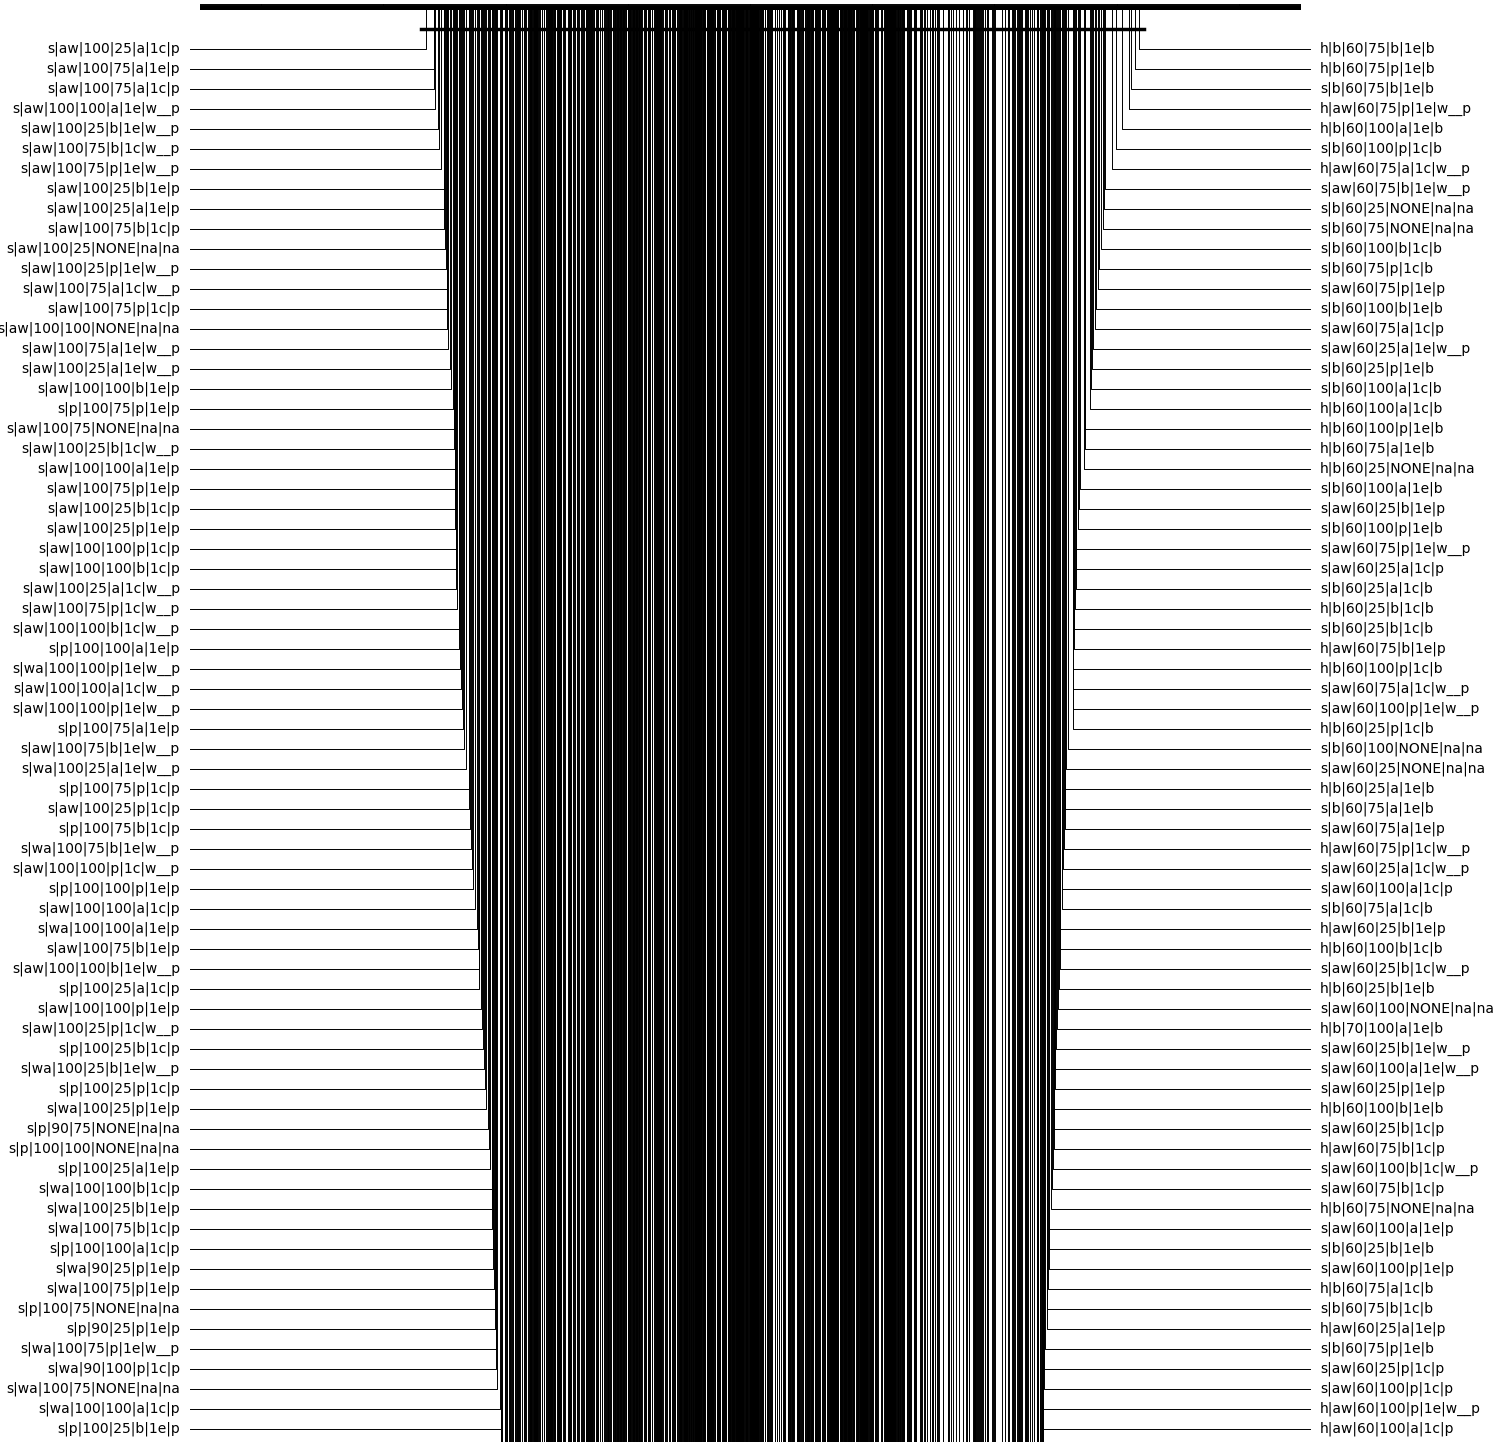
\includegraphics[width=\linewidth]{./images/rank_kappa_cropped}
\caption{\label{fig:rank_kappa}Ranking all parameter combinations, over $\kappa_t$}
\end{figure}
\begin{table}[]
\centering
\caption{\label{table:rank_kappa_breakdown}Breakdown of parameter value frequency in the top 50 ranked parameter combinations for $\kappa_t$}
\begin{tabular}{|l|c|c|}
\hline
\textbf{Parameter} & \textbf{Value} & \textbf{Breakdown} \\ \hline \hhline{===}
\multirow{2}{*}{Sliding type} & h & 10\% \\ \cline{2-3} 
 & s & 90\% \\ \hline
\multirow{3}{*}{Voting type} & aw & 36\% \\ \cline{2-3} 
 & p & 26\% \\ \cline{2-3} 
 & wa & 38\% \\ \hline
\multirow{2}{*}{Ground truth} & 90 & 38\% \\ \cline{2-3} 
 & 100 & 62\% \\ \hline
\multirow{3}{*}{Batch size} & 25 & 34\% \\ \cline{2-3} 
 & 75 & 38\% \\ \cline{2-3} 
 & 100 & 28\% \\ \hline
\multirow{4}{*}{Drift reset type} & a & 26\% \\ \cline{2-3} 
 & b & 26\% \\ \cline{2-3} 
 & n & 12\% \\ \cline{2-3} 
 & p & 36\% \\ \hline
\multirow{3}{*}{Detector count} & 1c & 42\% \\ \cline{2-3} 
 & 1e & 46\% \\ \cline{2-3} 
 & none & 12\% \\ \hline
\multirow{3}{*}{Detector content} & p & 68\% \\ \cline{2-3} 
 & wp & 20\% \\ \cline{2-3} 
 & none & 12\% \\ \hline
\end{tabular}
\end{table}

Table \ref{table:rank_kappa_breakdown} indicates how frequently each parameter occurred in the top 50 ranked parameter combinations for $\kappa_t$. These results suggest that parameter combinations with the following values to score higher on the $\kappa_t$ metric: [\textit{sliding, *, $100\%$, 75 or 25, partial, 1c or 1e, probability}]. The asterisk is used to indicate any value for that parameter.
These findings don't exactly match up with the results found in the previous section. For example, we found that probability voting was more likely to be top ranking in the previous section, whereas we found in this section that weighted averaged or averaged weighted probability voting was more frequently in the 50 top ranked parameter combinations. The same can be said for the drift reset type parameter value.

\subsection{Ranking over execution time}
Figure \ref{fig:rank_seconds} shows the post-hoc Nemenyi ranking results for the execution time metric. As before, the left hand side lists the best ranking parameter combinations, and the right hand side shows the worst performing ones. 
We'll consider the 50 top ranking parameter combinations.

\begin{figure}
  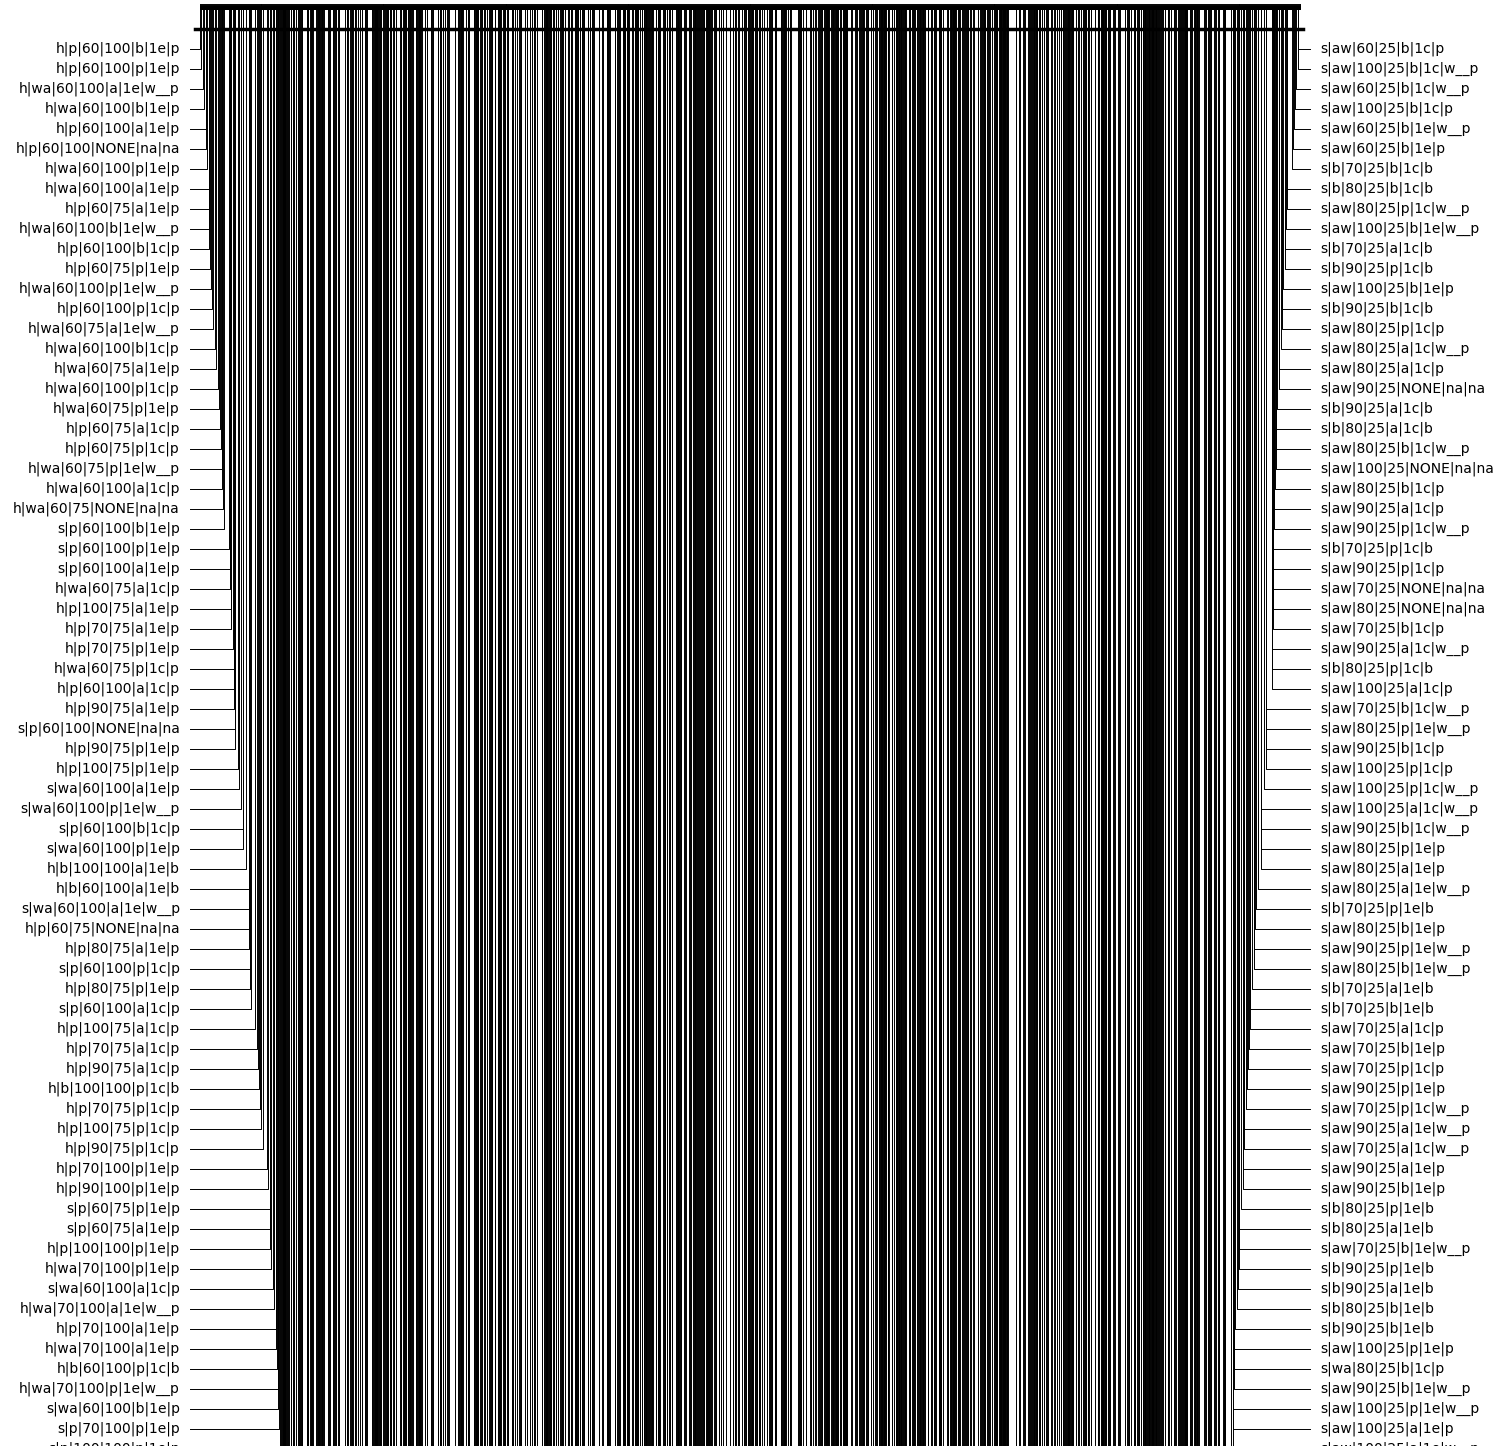
\includegraphics[width=\linewidth]{./images/rank_seconds_cropped}
\caption{\label{fig:rank_seconds}Ranking all parameter combinations, over execution time}
\end{figure}
\begin{table}[]
\centering
\caption{\label{table:rank_seconds_breakdown}Breakdown of parameter value frequency in the top 50 ranked parameter combinations for execution time}
\begin{tabular}{|l|c|c|}
\hline
\textbf{Parameter} & \textbf{Value} & \textbf{Breakdown} \\ \hline \hhline{===}
\multirow{2}{*}{Sliding type} & h & 78\% \\ \cline{2-3} 
 & s & 22\% \\ \hline
\multirow{4}{*}{Voting type} & aw & 0\% \\ \cline{2-3} 
 & b & 4\% \\ \cline{2-3} 
 & p & 56\% \\ \cline{2-3} 
 & wa & 40\% \\ \hline
\multirow{5}{*}{Ground truth} & 60 & 80\% \\ \cline{2-3} 
 & 70 & 4\% \\ \cline{2-3} 
 & 80 & 4\% \\ \cline{2-3} 
 & 90 & 4\% \\ \cline{2-3} 
 & 100 & 8\% \\ \hline
\multirow{3}{*}{Batch size} & 25 & 0\% \\ \cline{2-3} 
 & 75 & 42\% \\ \cline{2-3} 
 & 100 & 58\% \\ \hline
\multirow{4}{*}{Drift reset type} & a & 42\% \\ \cline{2-3} 
 & b & 14\% \\ \cline{2-3} 
 & p & 36\% \\ \cline{2-3} 
 & none & 8\% \\ \hline
\multirow{3}{*}{Detector count} & 1c & 28\% \\ \cline{2-3} 
 & 1e & 64\% \\ \cline{2-3} 
 & none & 8\% \\ \hline
\multicolumn{1}{|c|}{\multirow{4}{*}{Detector content}} & b & 4\% \\ \cline{2-3} 
\multicolumn{1}{|c|}{} & p & 74\% \\ \cline{2-3} 
\multicolumn{1}{|c|}{} & wp & 14\% \\ \cline{2-3} 
\multicolumn{1}{|c|}{} & none & 8\% \\ \hline
\end{tabular}
\end{table}

Table \ref{table:rank_seconds_breakdown} indicates how frequently each parameter occurred in the top 50 ranked parameter combinations for the execution time. These results suggest that parameter combinations with the following values to have lower values for the execution time metric: [\textit{hybrid, probability, $60\%$, 100, partial, 1c or 1e, probability}]. These results almost completely match the results from the previous section, confirming our findings.

\subsection{Ranking over both metrics}

By filtering the raw values from the simulations we ran, in combination with the rankings obtained in the two previous subsections, the best performing parameter combinations will be determined in this subsection.

Figure \ref{fig:rank_both_all} shows the raw values for each data set for both measured metrics. The values are ordered by an average of the ranks for $\kappa_t$ and execution time. To give more weight to the predictive accuracy in the ordering, the equation for the average is the following: $\frac{3\times rank_{\kappa_t}+rank_{execution\ time}}{4}$.

\begin{figure}
  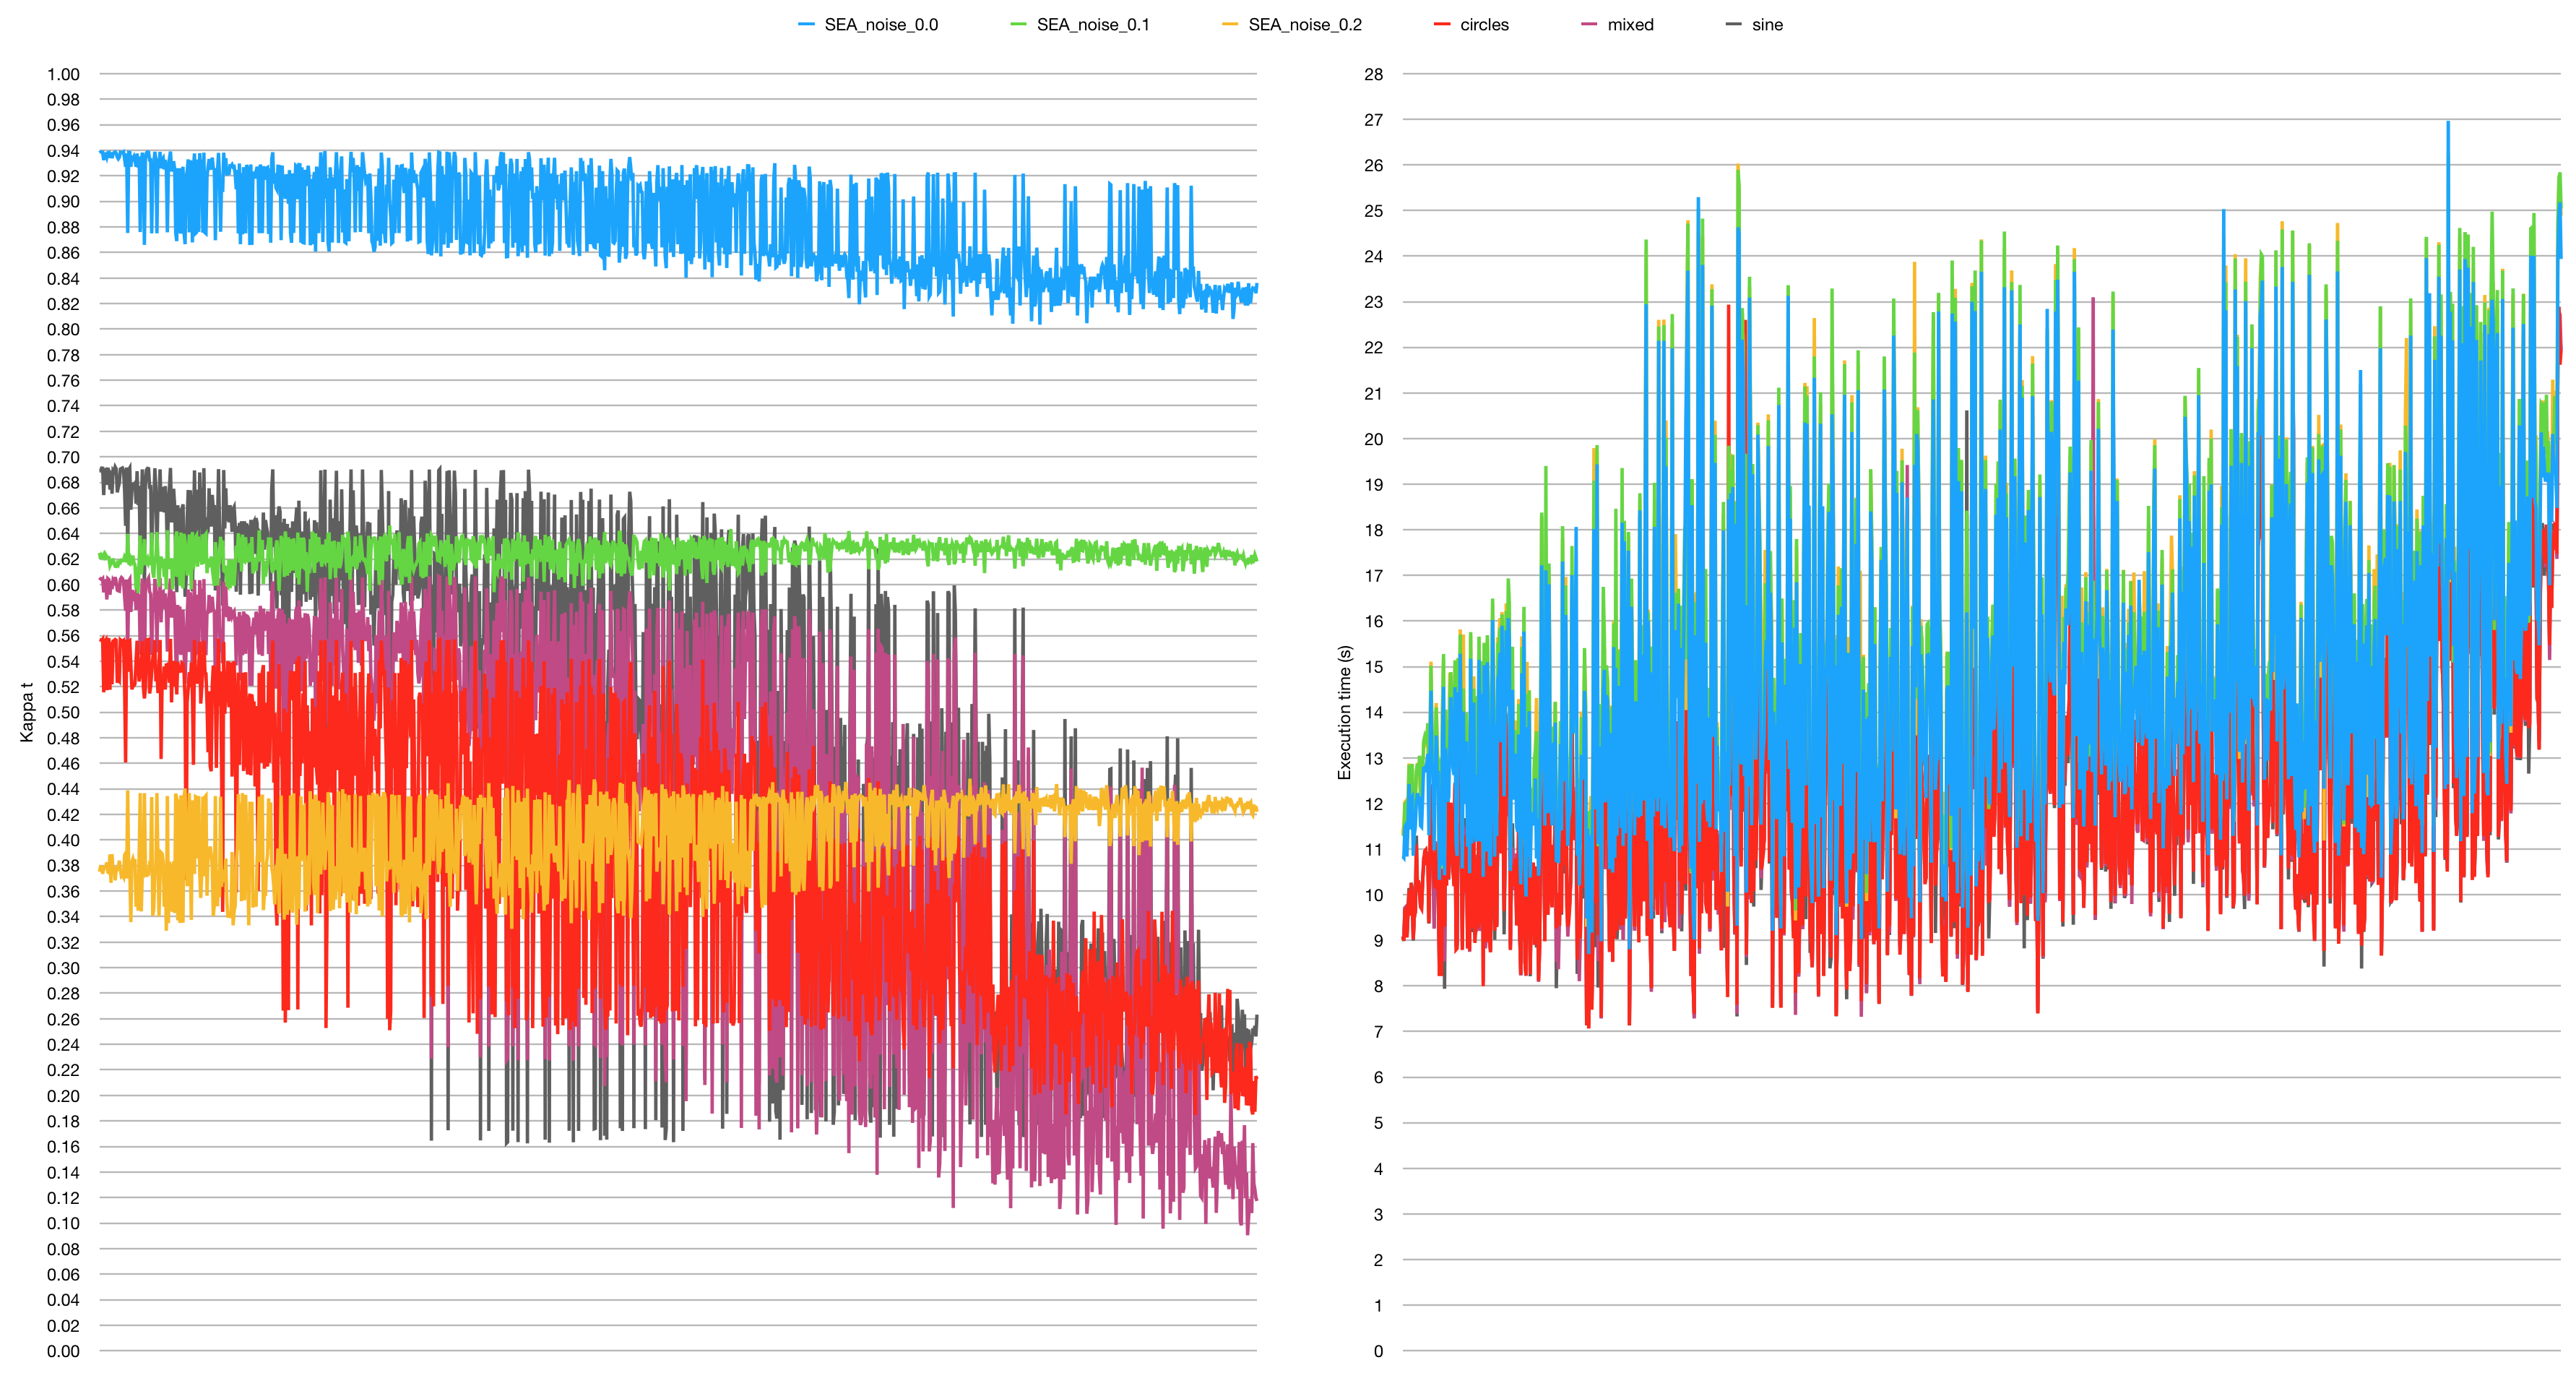
\includegraphics[width=\linewidth]{./images/rank_both}
\caption{\label{fig:rank_both_all}Raw $\kappa_t$ and execution time values ordered by averaged ranks}
\end{figure}

In order to find the right balance, we started to filter out the parameter combinations with the conditions found in table \ref{table:rank_both_filter_dataset}, and then filtered out those whose averaged rank was below 340. We should note that the $\kappa_t$ ranks are in the range of $[228.8, 947.3]$ and that of the execution time in the range of $[1, 1108.2]$. Figure \ref{fig:compare_both_best} shows the remaining parameter combinations, with their raw values for both measured metrics. These filters were selected by intuition and through extensive exploration and inspection, in order to remove very high execution times as well as poor $\kappa_t$ values. We also chose to include the parameter combinations that led to the best overall $\kappa_t$ average metric, and the one with the best average execution time metric.

\begin{table}[]
\centering
\caption{\label{table:rank_both_filter_dataset}Data set filtering conditions}
\begin{tabular}{|l|c|} 
\hline
\textbf{Data set} & \textbf{Condition} \\ \hline \hhline{==}
SEA $0\%$ noise & $\le$ 11 seconds \\ \hline
circles & $\le$ 9.2 seconds \\ \hline
sine & $\le$ 9.2 seconds \\ \hline
mixed & $\le$ 9.1 seconds \\ \hline
\end{tabular}
\end{table}

\begin{figure}
  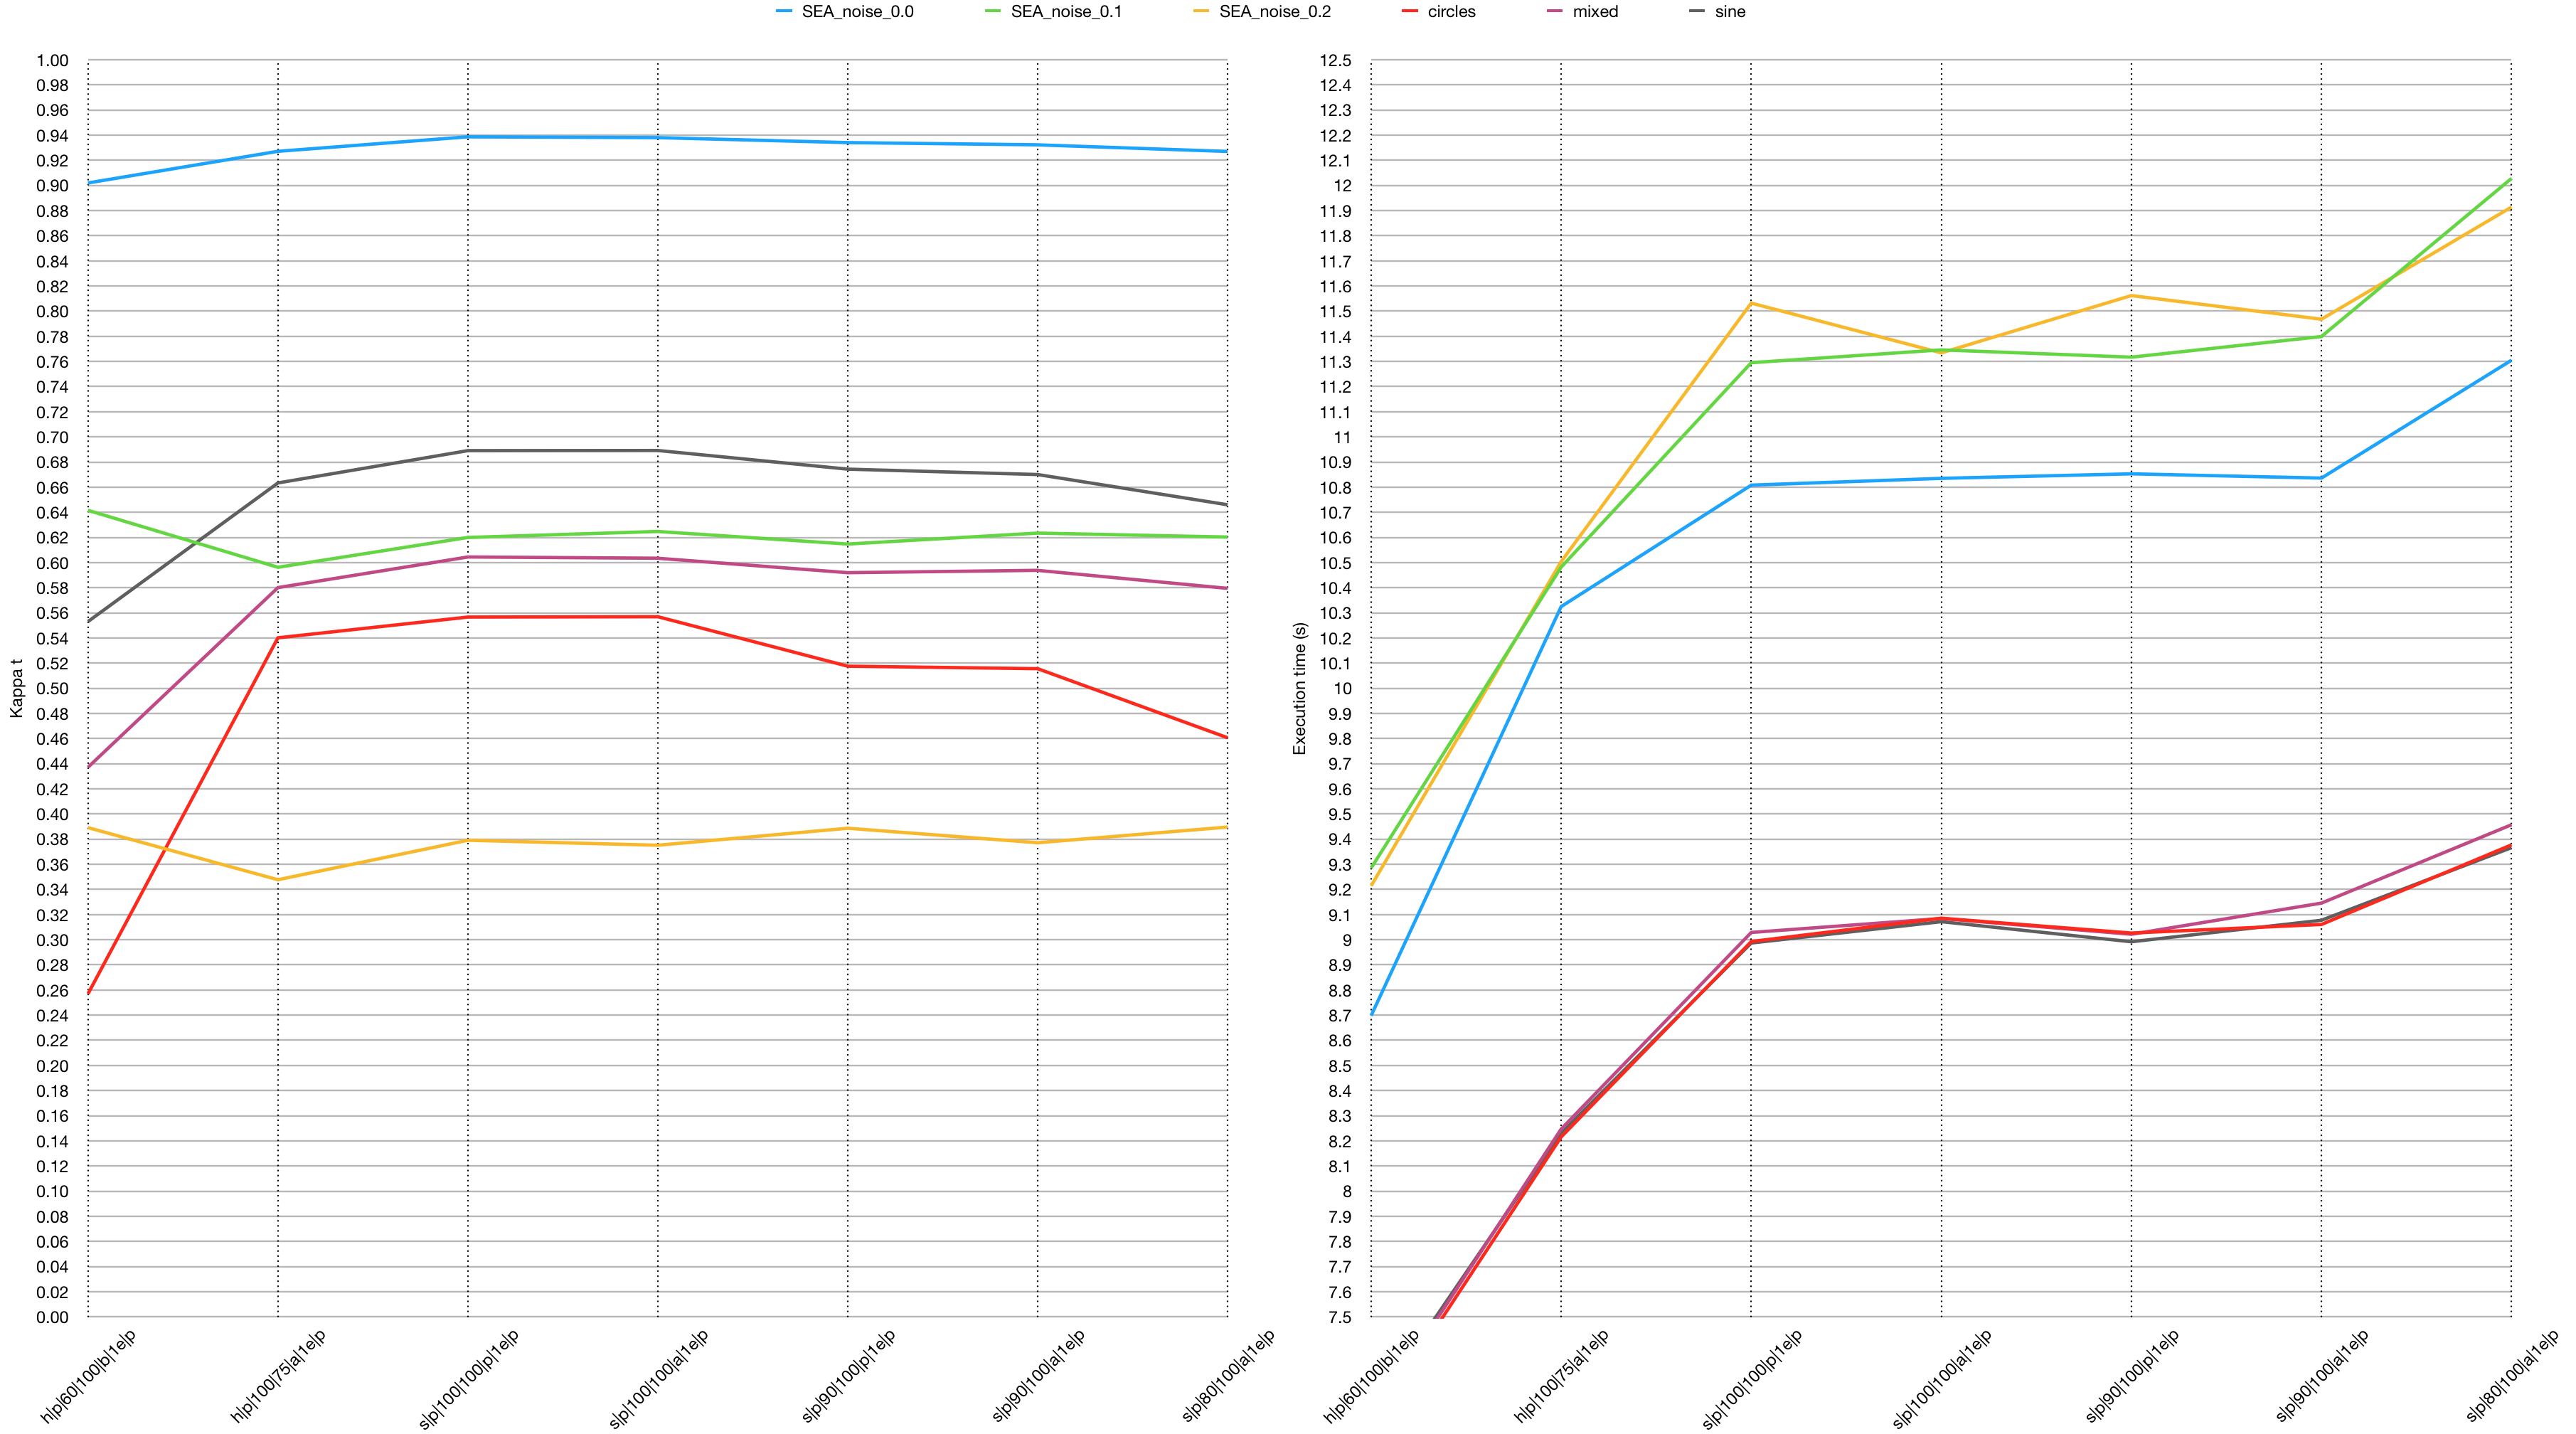
\includegraphics[width=\linewidth]{./images/compare_both_best}
\caption{\label{fig:compare_both_best}Remaining parameter combinations and their raw metric values after filtering}
\end{figure}

For the best resulting predictive accuracy, [\textit{sliding window, probability voting, $100\%$ ground truth, 100 batch size, partial reset, 1 drift detector, probability drift content}] proved to be the best parameter combination. And for the best execution time,  the following combination of parameters proved to be the best: [\textit{hybrid window, probability, $60\%$ ground truth, 100 batch size, blind reset, 1 drift detector, probability content}]. 

However, if we can accept a $1$ to $4\%$ reduction for $\kappa_t$ values, then significant time savings can be achieved by using [\textit{hybrid window, probability voting, $100\%$ ground truth, 75 batch size, reset all, 1 drift detector, probability content}]. Indeed, we can reduce execution time by up to $9.5\%$.

\subsection{Effects of reducing ground truth used for training}
As stated in section \ref{section:vc_reduce_gt}, we want to determine at what ratio of predictions to ground-truth our voting ensemble's prediction accuracy declines and by how much. Figure \ref{fig:ground_truth_drop} shows examples of parameter combinations using varying amounts of ground truth ($10\%$ increments starting at 60). The values shown in the graphs were selected manually after having been ranked with the averaging equation shown above. The selection process was simple, we selected one or two parameter combinations that had the highest averaged rank value for a given percentage of ground truth. The graph indicates that the predictive accuracy of our ensemble doesn't drop until we use $80\%$ of ground truth. The execution times can be reduced by further reducing the predictive accuracy.

One finding that we find particularly odd is that as the use of ground truth diminishes, the predictive accuracy increases for the SEA generated data sets with noise. We are led to believe that for increasing levels of noise in a data set, reducing the ground truth used (to an extent) to train a model increases its predictive accuracy. Further research, outside the scope of this thesis, is needed to ascertain the veracity of this finding.

\begin{figure}
  \includegraphics[width=\linewidth]{./images/chapter5/ground_truth}
\caption{\label{fig:ground_truth_drop}$\kappa_t$ and execution times for parameter combinations using varying amounts of ground truth}
\end{figure}

\section{Comparing to the State of the Art}

Now that we have determined which parameter combinations worked particularly well, we can compare them to the State of the Art.

As previously mentioned, the algorithms which we will be comparing our voting ensemble to will be mainly the Leveraging Bagging algorithm. As we explained in the previous chapter, the Leveraging Bagging will be comprised of 10 Hoeffding Tree estimators, each with its own ADWIN drift detector. We will also be using a regular Hoeffding Tree using the default parameters without any drift detector. Finally, we will also include a no-change and a majority class classifier in our comparison.

\subsection{Choosing a window size for State of the Art algorithms}

\begin{figure}
  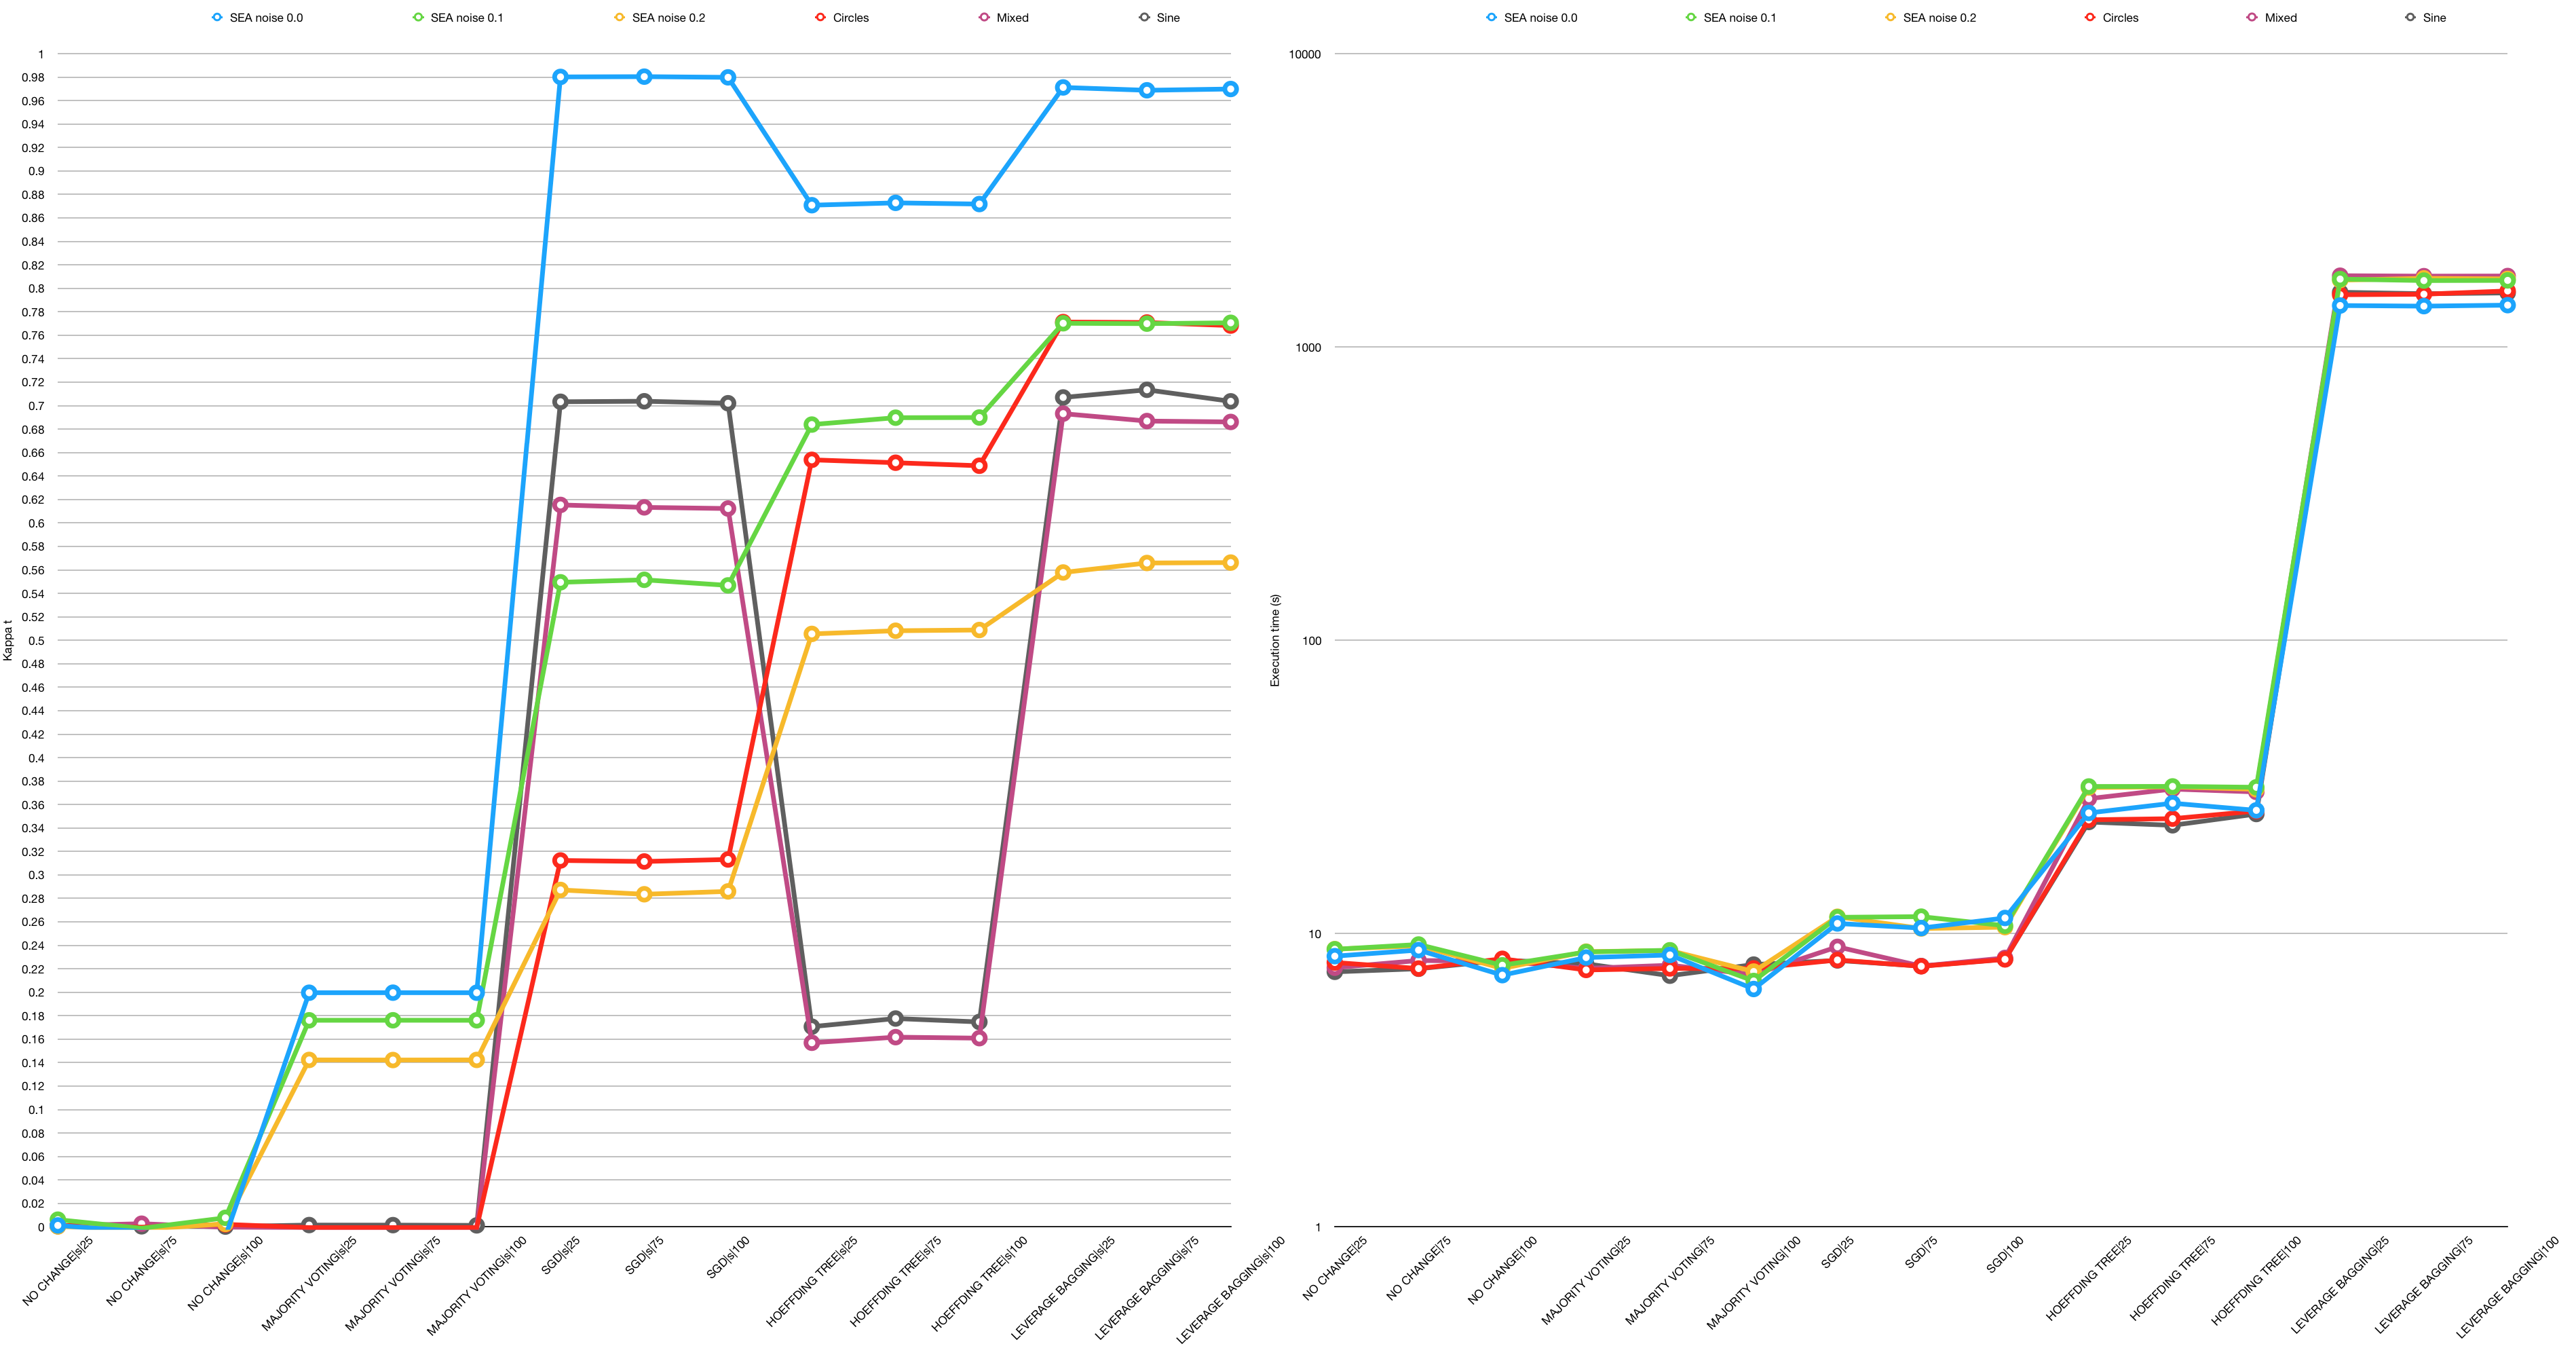
\includegraphics[width=\linewidth]{./images/chapter5/compare_sota}
\caption{\label{fig:raw_compare_sota}$\kappa_t$ and execution times of State of the Art algorithm with varying window sizes}
\end{figure}

For these algorithms, we made sure to use $100\%$ ground truth for the training, sliding windowing and only modified the window size. However, changing the window size did not change the execution times or $\kappa_t$ by much more than $1\%$ or 1 second as can be seen in figure \ref{fig:raw_compare_sota}. For this reason, we chose to simply keep one example for each algorithm, that ranked better with a given window size than other. We should note that applying the Friedman test and Nemenyi tests showed that the window size resulted in confirming the null hypothesis that all window sizes led to similar results for each classifier for the no change, majority voting, and SGD classifiers. Therefore, we simply took the best overall ranking window size. For Hoeffding Trees, window size of 25 showed a significant statistical difference to 100 but only for the execution time. For Leveraging Bagging, window size of 25 showed a significant statistical difference to 100 but only for the $\kappa_t$ metric.

The resulting chosen window sizes are as follows: no change (25),  majority voting (25), SGD (75), Hoeffding Tree (25), Leveraging Bagging (25).

We have opted to compare these algorithms to our voting ensemble with 6 different parameter combinations (1 for each increment of ground truth used, and an additional one using $100\%$ ground truth).


\subsection{Visual comparison}

Finally, we can compare our voting ensemble to the state of the art. Figure \ref{fig:raw_compare_sota_all} shows the raw results, to better visualize how each algorithm, and its parameter combinations affects the data sets that they are trying to model.

\begin{figure}
  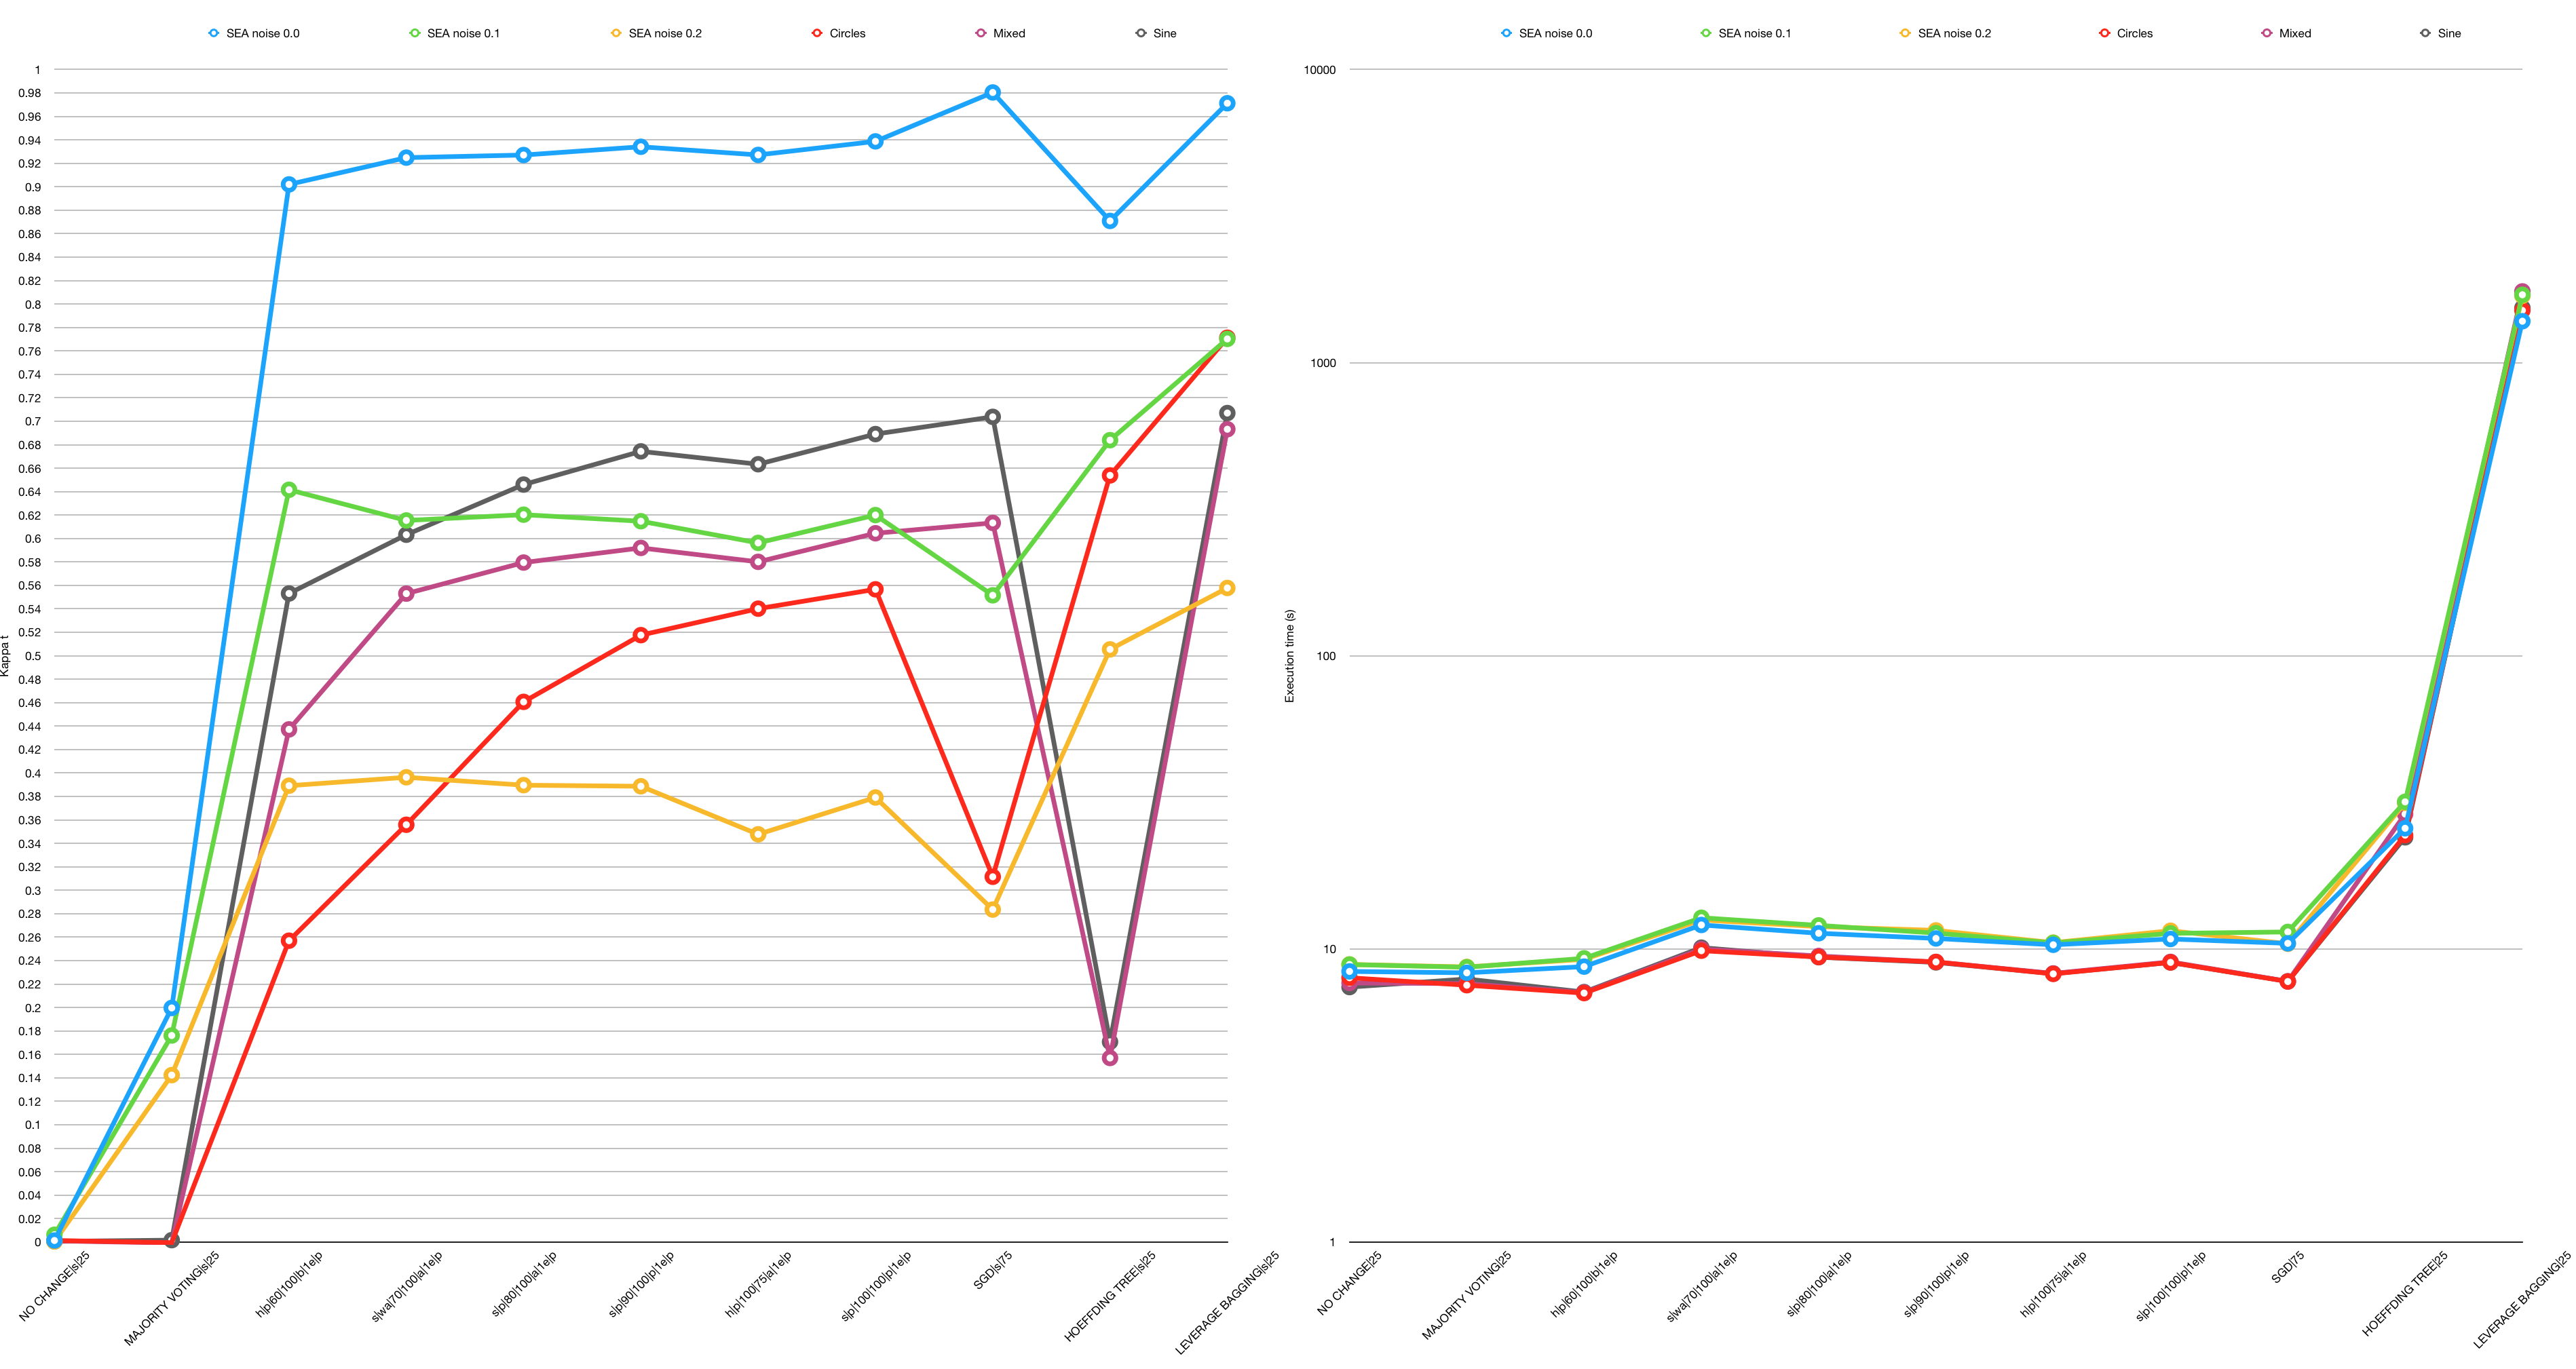
\includegraphics[width=\linewidth]{./images/chapter5/compare_sota_all}
\caption{\label{fig:raw_compare_sota_all}$\kappa_t$ and execution times when comparing our Voting Ensemble to the State of the Art}
\end{figure}

As we can see from these two graphs, Leveraging Bagging (LB) does achieve the best predictive accuracy but the worst execution time. While the difference in predictive accuracy between LB and the other algorithms is noticeable, it isn't glaring. However, when it comes to execution time, we were required to use a logarithmic scale to show its run time while also showing the run times of other algorithms. LB takes more than 2 orders of magnitude longer than the Voting Ensemble, and 1.5 order of magnitude longer than a Hoeffding Tree (HT). Given that LB is comprised of 10 HTs, it makes perfect sense that LB takes so much longer to run.

However, our findings from the graph do not have the weight of a proper statistical analysis, which follows in the next section.

\subsection{Statistical Analysis}
In this final section, we will test the following two null hypotheses:
\begin{enumerate}
\item all algorithms, with their respective parameters predict classes equally well ($\kappa_t$)
\item all algorithms, with their respective parameters run in an equal amount of time.
\end{enumerate}

\subsubsection{For $\kappa_t$}

We will start with the first, using the $\kappa_t$ metric. Again, the Friedman test was used, with a significance level of 0.05. We found that $p < 2.1\times10^{-23}$, thus rejecting the null hypothesis.
To determine which pairs of algorithms actually differ, we used the post-hoc Nemenyi test, yet again. The results can be seen in figure \ref{fig:sota_compare_all_kappa_nemenyi}, where a lower rank means a better predictive accuracy (a better $\kappa_t$).

\begin{figure}
  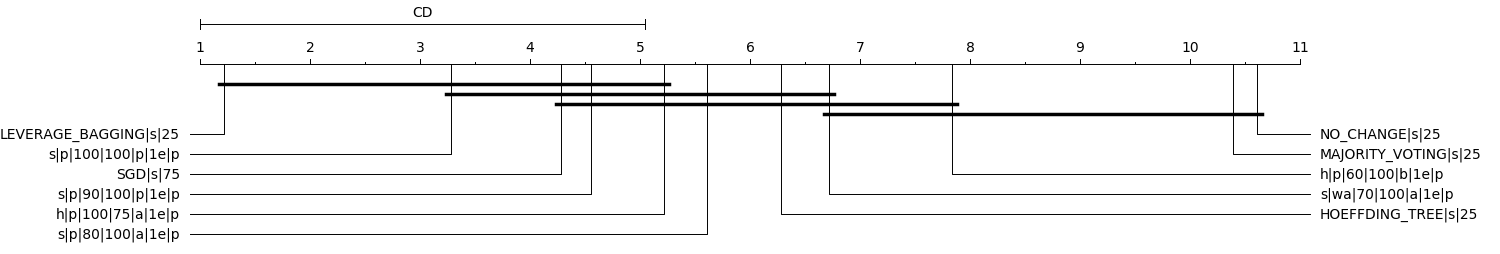
\includegraphics[width=\linewidth]{./images/chapter5/sota_compare_all_kappa_nemenyi}
\caption{\label{fig:sota_compare_all_kappa_nemenyi}Nemenyi graph ranking $\kappa_t$ for various algorithms}
\end{figure}

A Nemenyi graph shows a ranking of algorithms on a scale from 1 to N (typically the number of algorithms compared). A bar labelled critical difference (CD) is shown above the scale, which is the minimum rank length for two algorithms to not show a significant statistical difference in rank. 
Additionally, there may be horizontal bars that link ranked algorithms. Any algorithms that share a same horizontal bar are not significantly statistically different. Pairs of algorithms that are further apart than the CD bar are significantly statistically different.

We can see from the graph that there is not significant statistical difference between LB, our Voting Ensemble using our best overall parameter combination, an SGD classifier, our Voting Ensemble using our hybrid windowing approach, and our Voting Ensemble using only $80\%$ ground truth when training. This confirms the rejection of the null hypothesis for $\kappa_t$. It's also a very good sign, because all of the above mentioned algorithms were statistically significantly better than a single Hoeffding Tree.

As a side note, we can also say that there is a significant statistical difference between both the majority voting and no change classifiers with all algorithms, aside from our Voting Ensemble training with $70\%$ of ground truth or less.

Therefore, this test showed that our Voting Ensemble, using our preferred parameter combinations, did not perform better or worse, statistically speaking, than Leveraging Bagging.

\subsubsection{For execution time}

For the final measure, execution time, we use the Friedman test, with a significance level of 0.05. We found that $p < 1.68\times10^{-31}$, thus leaving no doubt as to the rejection of the null hypothesis. The post-hoc Nemenyi test is used to determine which pairs of algorithms differ. The Nemenyi graph is shown in figure  \ref{fig:sota_compare_all_execution_time_nemenyi}, where a lower rank means a lower execution time.

\begin{figure}
  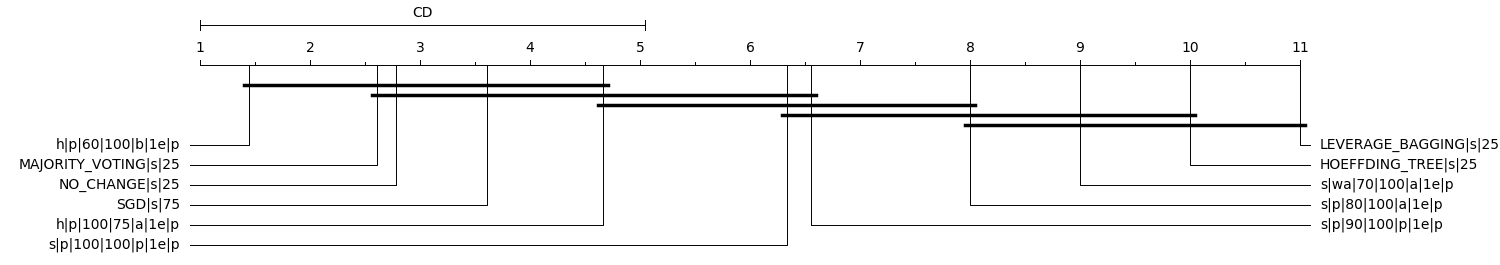
\includegraphics[width=\linewidth]{./images/chapter5/sota_compare_all_execution_time_nemenyi}
\caption{\label{fig:sota_compare_all_execution_time_nemenyi}Nemenyi graph ranking execution times for various algorithms}
\end{figure}

We can see from the graph that Leveraging Bagging ranks last, and Hoeffding Trees ranks second last, which is as expected given the raw values that we saw above. 
The graph also shows that there is a significant statistical difference between Leveraging Bagging (the State of the Art algorithm we're comparing), and our Voting Ensemble (except when using $70\%$ or $80\%$ ground truth). Given that Leveraging Bagging runs in over 2 orders of magnitude longer than our Voting Ensemble, this result is not surprising in the least. It is, however, comforting to have our visual analysis backed by this statistical test.

Therefore, this test statistically showed that our Voting Ensemble runs significantly faster than Leveraging Bagging.

Additional graphs (statistical significance heatmaps and more Nemenyi graphs) can be seen in the appendix: \ref{section:nemenyi-graphs-statistical-analysis}.

\subsubsection{What do these results mean ?}
First of all, our statistical significance tests showed that our Voting Ensemble was able to outperform the State of the Art \textit{Leveraging Bagging} algorithm in execution time, and that it was able to perform on par with \textit{Leveraging Bagging} in regards to the $\kappa_t$ measured metric. It also showed that we could use only $90\%$ ground truth without compromising our Ensemble's predictive accuracy in comparison to \textit{Leveraging Bagging}.

Our algorithm therefore predicts on par with Leveraging Bagging and brings outstanding time savings in algorithm run-time, running somewhere over 160 times faster.

Practically, this means that ensembles should definitely be considered when execution time is an important metric. However, for the applications that strictly require high predictive accuracy, Leveraging Bagging would still be the valid choice.

\section{General discussion and conclusion}

% Chapter 6

\chapter{Conclusion\label{chapter:conclusion}} % Main chapter title

%----------------------------------------------------------------------------------------

This thesis focused on improving semi-supervised learning from evolving streams without the use of clustering techniques, which are computationally expensive \cite{krempl2014open}. The goal of this study was to design fast algorithms to work with fewer labelled examples, and to extend an existing algorithm to detect drifts without relying on ground truth. Experiments were conducted in order to compare the performance of our framework against that of the state of the art in terms of predictive accuracy and execution time, while considering the percentage of labelled instances used at each stage of learning. This chapter discusses our contributions and presents opportunities for future work.

%----------------------------------------------------------------------------------------
 
\section{Contributions}
A great deal of research is being conducted to develop algorithms for supervised learning of evolving streams. These techniques are usually ensemble-based, and typically make use of either boosting or bagging. This research is necessary to understand how well an algorithm can learn from an evolving stream, but the use of supervised training is to online learning as training wheels are to learning how to ride a bicycle. In the real-world, the assumption that true labels will arrive on time is unequivocally unreasonable. We introduce our semi-supervised hybrid-windowing ensembles for learning in evolving streams as our solution to deal with this issue without using clustering techniques.

We first proposed a voting ensemble that uses a modified soft voting approach, by weighting each classifier’s predictive confidence. Next, we developed a novel windowing type for ensembles, as sliding windows are very time consuming and regular tumbling windows are not a suitable replacement. Our windowing technique can be considered a hybrid of the two: we train each sub-classifier in the ensemble with tumbling windows, but delay training in such a way that only one sub-classifier can update its model per iteration. We also extended selective self-training by ignoring its heuristic: training classifiers using all predicted examples, and not only those with high predictive confidence. Finally, we extended an existing concept drift detector to successfully operate without any labelled data, by using a sliding window of our ensemble’s prediction confidence, instead of a boolean value indicating whether, or not, the ensemble predicted correctly.

%----------------------------------------------------------------------------------------

\section{Future Work}
Our framework took very little execution time, far below that of a current state of the art technique, and achieved comparable predictive accuracy to that of state of the art techniques that trained on fully-labelled data sets, while ours only trained on a subset of those labels, and ignoring them completely for detecting drifts. We believe that a higher predictive accuracy can be achieved without significantly impacting the execution time, even when training with less labelled data.

In order to reduce the quantity of labelled data used for (pre-)training, we can introduce specialised domain knowledge into the learning cycle. An interactive active learning approach can be used, as seen in \cite{floyd2017activetext}, where an intuitive online interface is used to request labels, from an oracle, for any number of uncertain data instances to train on instances that are representative of the stream, or those that classifiers find difficult.

Furthermore, our framework can be improved by incorporating ideas that have been proven to work such as intelligent window sizes, and replacing classifiers with a bad predictive accuracy streak. To deal with recurring concepts, we can incorporate weighted summarising classifiers as seen in Learn$^{++}$.NSE \cite{elwell2011incremental}, however, the memory issue would need to be addressed.

Additionally, our framework does not guarantee diversity among the classifiers in the ensemble. A possible approach would be to replace the cyclic training from hybrid windows with a stochastic method. In other words, instead of training the classifiers in the ensemble in the same cyclical sequential manner, a classifier would be chosen at random to be trained from the new hybrid window.

Another area to be explored is how our framework performs when dealing with mixed concept drifts, and perform a study using a real-world data set.

Finally, our framework can be extended to better deal with unbalanced datasets. This would increase its applicability to real-world problems such as intrusion detection, and fraud detection.

%----------------------------------------------------------------------------------------
%	THESIS CONTENT - APPENDICES
%----------------------------------------------------------------------------------------

\appendix % Cue to tell LaTeX that the following "chapters" are Appendices

% Include the appendices of the thesis as separate files from the Appendices folder
% Uncomment the lines as you write the Appendices

% \include{Appendices/AppendixA}
%\include{Appendices/AppendixB}
%\include{Appendices/AppendixC}
\chapter{Graphs} % Main chapter title

\label{Appendix}

%----------------------------------------------------------------------------------------

\section{\label{section:nemenyi-graphs-statistical-analysis}Nemenyi Graphs}

\begin{figure}
  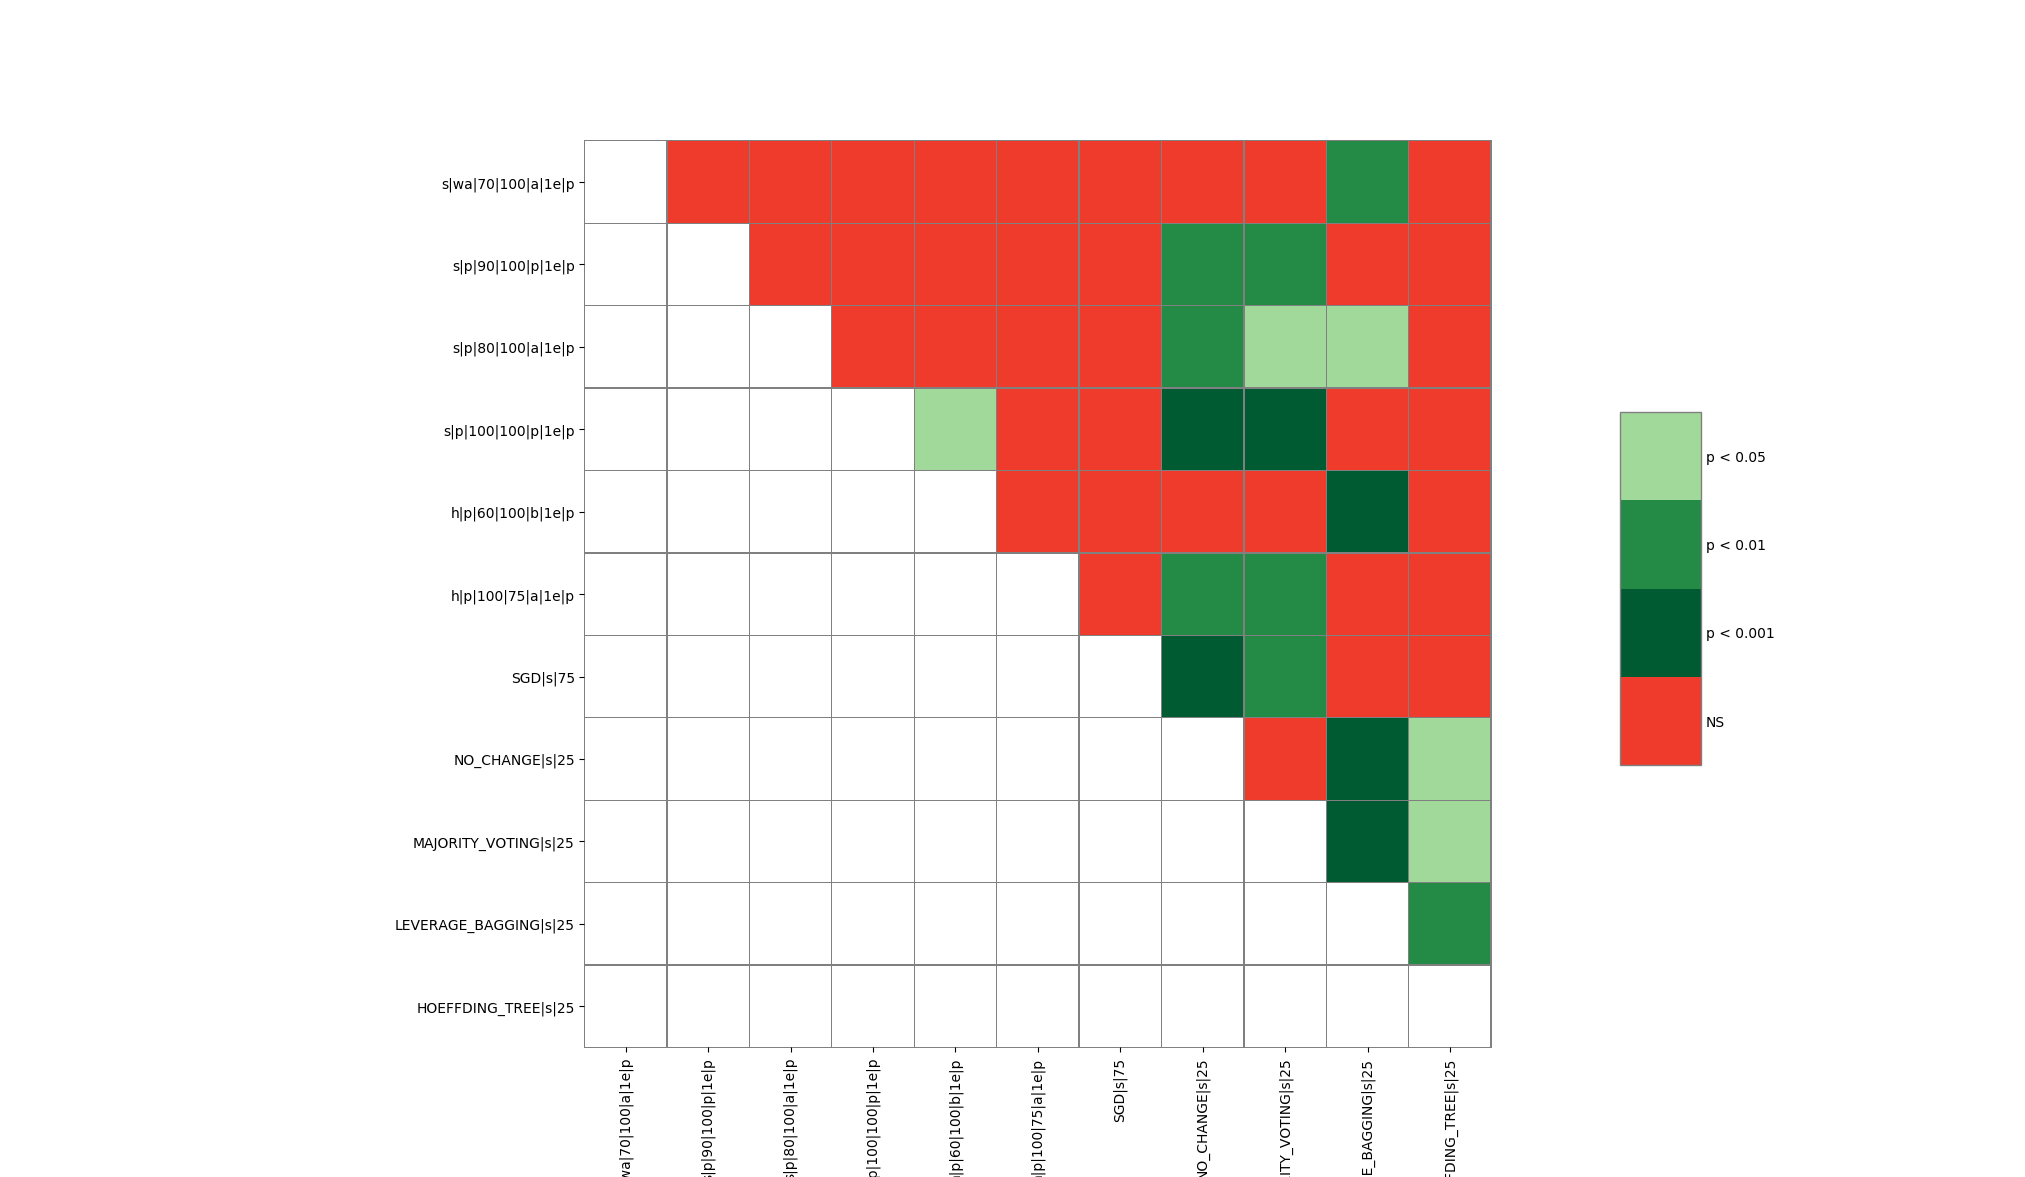
\includegraphics[width=\linewidth]{./images/appendix/heatmap_nemenyi_graphs/kappa_t_heatmap}
\caption{\label{fig:sota_kappa_t_heatmap}State of the Art comparison: $\kappa_t$ heatmap}
\end{figure}

\begin{figure}
  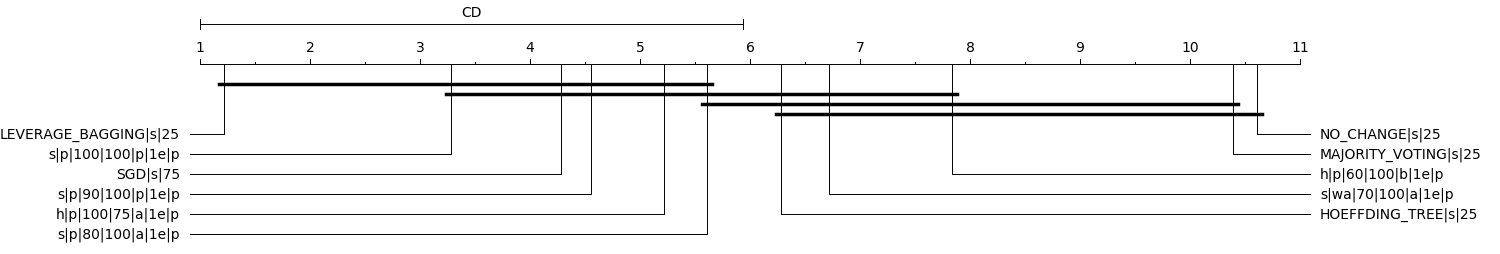
\includegraphics[width=\linewidth]{./images/appendix/heatmap_nemenyi_graphs/sota_compare_all_kappa_nemenyi__0_99}
\caption{\label{fig:sota_kappa_t_099}State of the Art comparison: post-hoc Nemenyi graph for $\kappa_t$, $\alpha=0.01$}
\end{figure}

\begin{figure}
  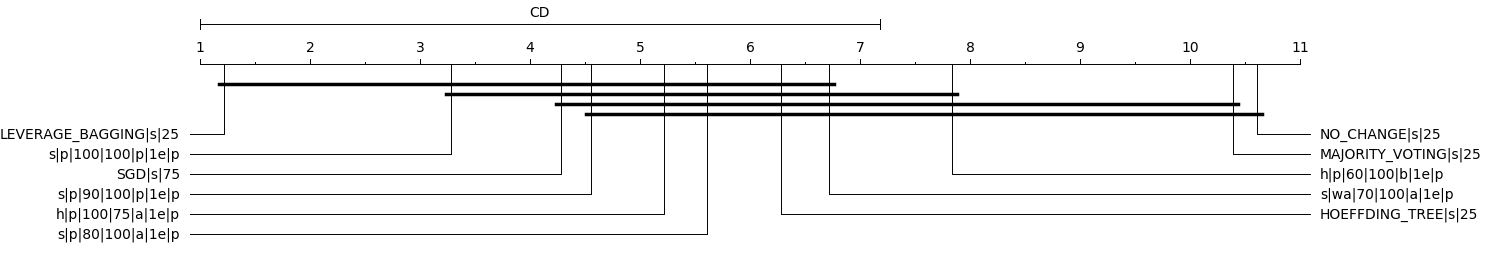
\includegraphics[width=\linewidth]{./images/appendix/heatmap_nemenyi_graphs/sota_compare_all_kappa_nemenyi__0_999}
\caption{\label{fig:sota_kappa_t_0999}State of the Art comparison: post-hoc Nemenyi graph for $\kappa_t$, $\alpha=0.001$}
\end{figure}

\begin{figure}
  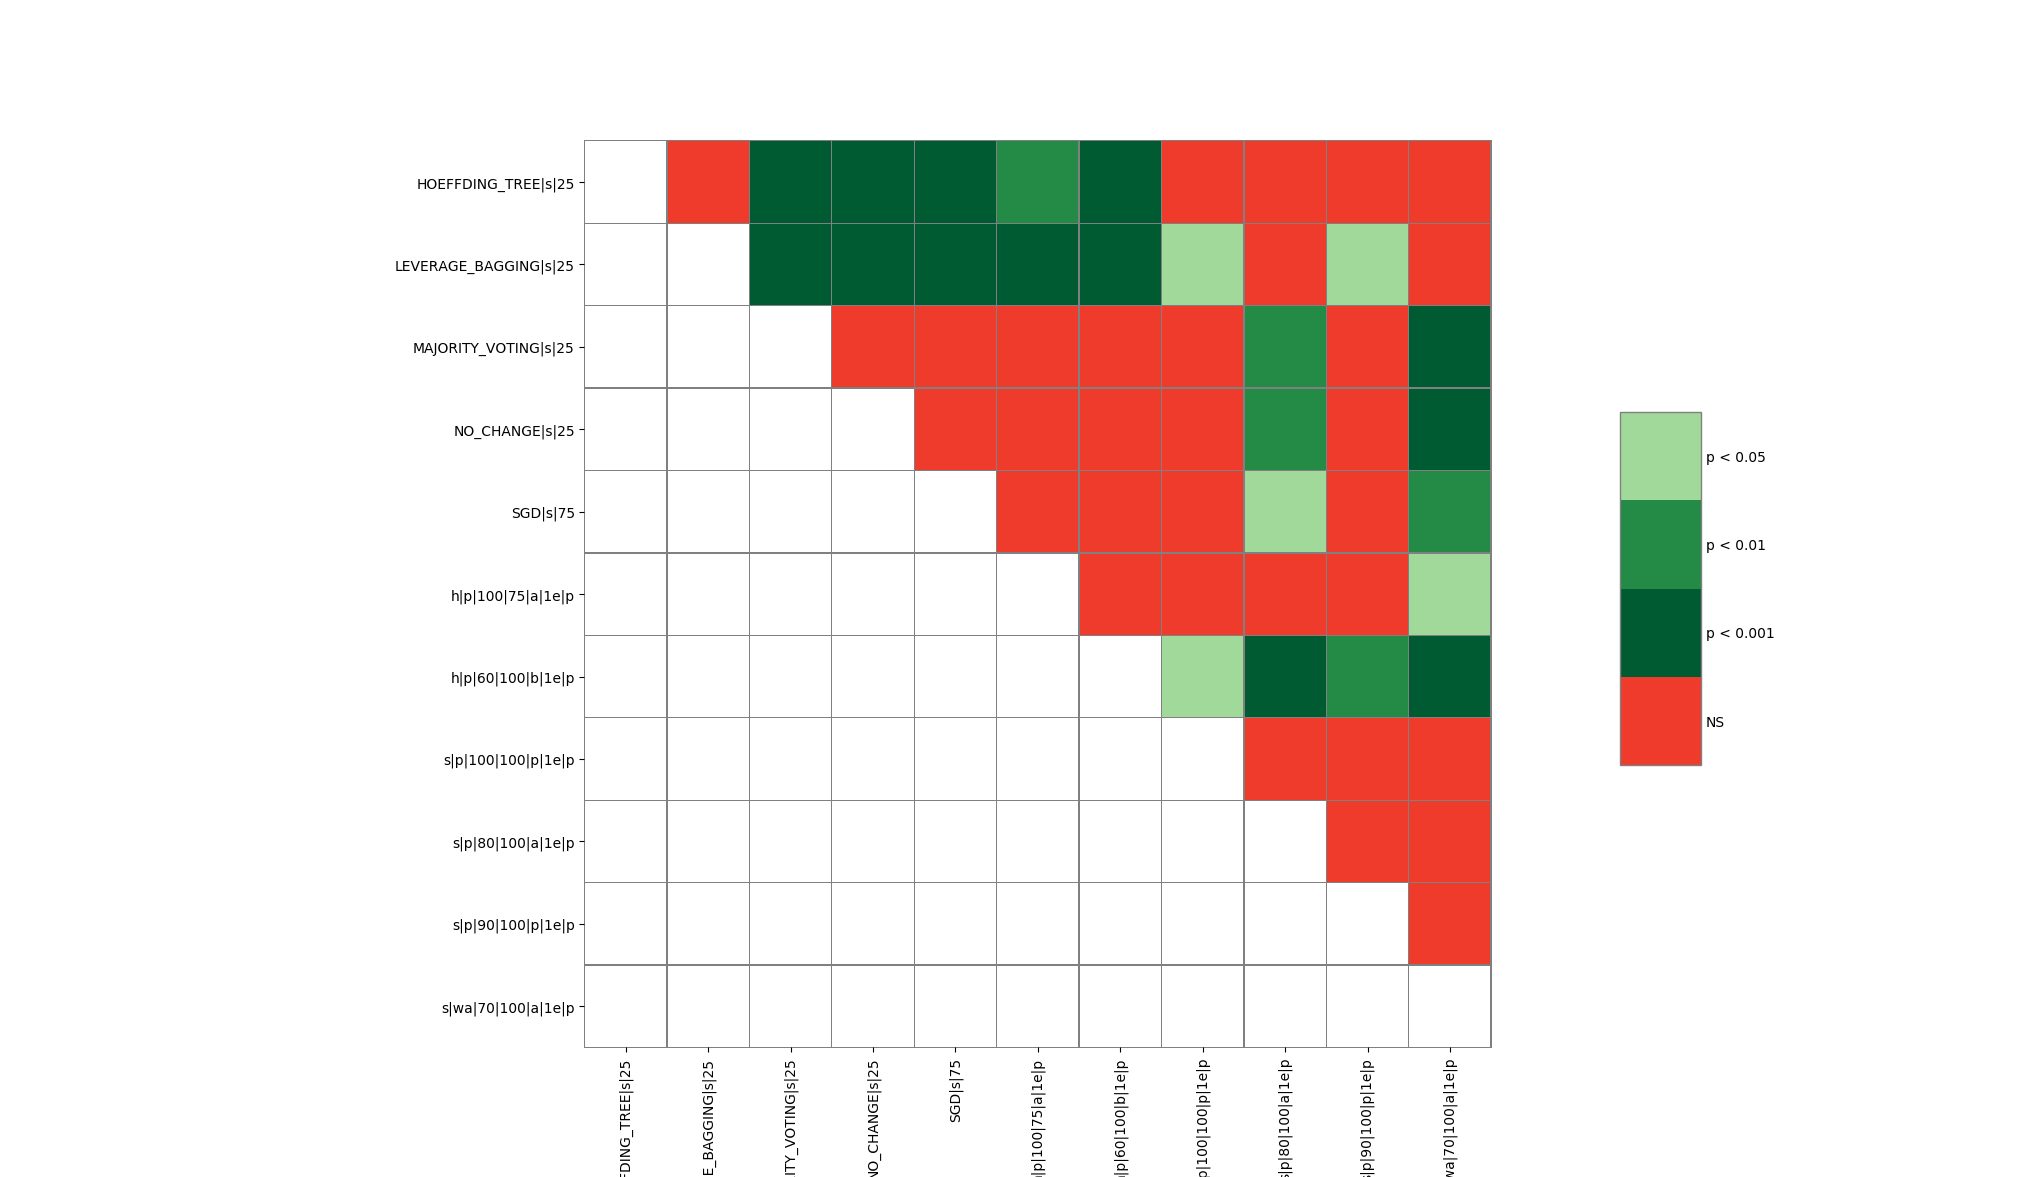
\includegraphics[width=\linewidth]{./images/appendix/heatmap_nemenyi_graphs/seconds_heatmap}
\caption{\label{fig:sota_seconds_heatmap}State of the Art comparison: execution time heatmap}
\end{figure}

\begin{figure}
  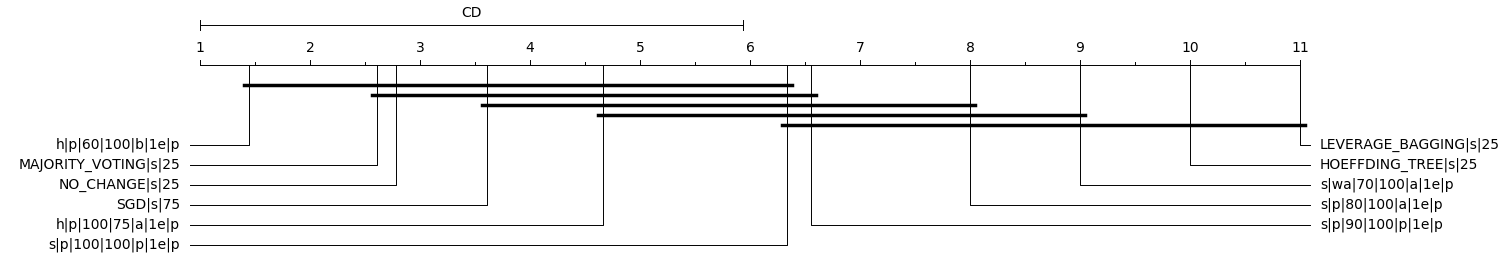
\includegraphics[width=\linewidth]{./images/appendix/heatmap_nemenyi_graphs/sota_compare_all_execution_time_nemenyi__0_99}
\caption{\label{fig:sota_seconds_099}State of the Art comparison: post-hoc Nemenyi graph for execution time, $\alpha=0.01$}
\end{figure}

\begin{figure}
  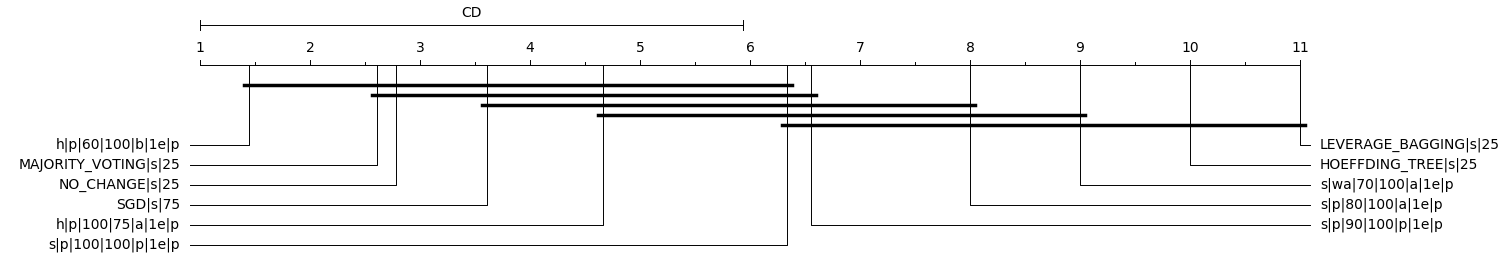
\includegraphics[width=\linewidth]{./images/appendix/heatmap_nemenyi_graphs/sota_compare_all_execution_time_nemenyi__0_99}
\caption{\label{fig:sota_seconds_0999}State of the Art comparison: post-hoc Nemenyi graph for execution time, $\alpha=0.001$}
\end{figure}

\chapter{Summaries}
As recommended by Silyn in \cite[p.~151]{silyn2012writing}, we have created this chapter to collect all of the chapter summaries.

%\section{Chapter \ref{chapter:introduction}: Introduction}

\section{Chapter \ref{chapter:background_work}: Background Work}
This chapter presents the fundamentals of machine learning and the various challenges of extracting knowledge from data streams. We introduce classification as a type of machine learning, for which the goal is to extract knowledge, computationally, from labelled data. Algorithms are developed to model the relationship between the data and the class labels. Semi-supervised learning is also a classification task but with the added constraint of learning from a data set that is not entirely labelled. In this thesis, the data we learn from come from data streams, which are voluminous, volatile and velocious. As such, constraints on time and memory usage must be respected, and a mechanism is required to forget "old data" safely.

We cover specific classifiers: baseline classifiers are usually relatively simple and used as a baseline for comparing classifier performance. We also cover the algorithms that we employed in our framework, as well as the state of the art: Naive Bayes, Stochastic Gradient Descent, Hoeffding Trees and Leveraging Bagging.

We define concept drifts as an evolution in the probability distribution of classes and/or attributes. We describe the main types of concept drifts that can occur, regardless of how self-explanatory they are named: abrupt, gradual and recurring. We then review drift detection strategies presented in the literature, including FHDDM/S which we extend in this thesis. Our review shows a gap in research as it pertains to semi-supervised drift detection.

Next, we define ensembles as an amalgamation of any number of classifiers. As all classifiers must output a prediction, ensembles must as well; we present existing techniques to map these multiple outputs to a single one. Having defined ensembles, we review those that were proposed in the literature using two criteria: the processing method and whether or not they were designed to deal with evolving concepts. The processing method distinguishes if instances are analyzed online (one-by-one) or in batches. Our review shows a gap in research as it pertains to semi-supervised learning from evolving streams.

We expect the audience of this thesis to be comfortable in the field of computer science and to have briefly read about or been introduced to machine learning.

\section{Chapter \ref{chapter:contributions}: Contributions}
In this chapter, we introduce our methodology, entitled Learning from Evolving Streams via Self-Training Novel Windowing Ensembles (LESS-TWE).

We propose a weighted soft voting scheme that uses a hyperbolic tangent function. We choose the $\tanh$ function as it allows us to approximate a logistic function while being less computationally expensive.

Next, we propose a novel windowing technique, exclusive to ensembles. Our technique allows every classifier in the ensemble to train from each data point in the stream \textbf{exactly once} similar to tumbling windows, as opposed to sliding windows where a data point is trained on \textbf{at least once}. As such, our method presents a trade-off between accuracy and execution time. Only one classifier per batch is trained on the window, therefor each classifier trains on a specific data instance at different times, resulting in delayed training. This means that only one classifier in the ensemble is trained on the newest data before the ensemble predicts labels for the subsequent batch.
The motivation for this technique is to determine if we can spend less execution time training the classifiers and to investigate how progressively delaying training of some of the classifiers in the ensemble affects concept drift detection and classification performance.

Our next contribution relates to selective self-training. In this semi-supervised learning algorithm, a classifier assigns a label it predicts to unlabelled data for future learning, if it is highly confident it is correct. There have not yet been any attempts, to the best of our knowledge, to investigate how self-training performs if labelling all unlabelled data, regardless of the classifier's confidence in its predicted label.

Finally, our last contribution is an extension of the Fast Hoeffding Drift Detecting Method for evolving data Streams. In our extension, instead of relying on the prequential accuracy, FHDDMS now makes use of an ensemble's or its classifiers' confidences, or of a boolean indicating if the classifier's and the ensemble's votes were identical for each classifier in the ensemble. Our extension allows FHDDMS to run without any labelled data, therefore making it an unsupervised drift detector.

Finally, we will cover all of our contributions by using a small toy example to explain how data is processed from a stream.

\section{Chapter \ref{chapter:experimental_design}: Experimental Design}
In this chapter, we describe how we conduct our experiments, on a MacBook Pro model \textit{11,4} running Python 3.7.3.

The data sets used for our analysis in the upcoming chapter comprise of generated SEA data with [0, 10, 20] percent noise as well as CIRCLES, SINE1 and MIXED data sets, which contain 10\% noise. Our data sets contain either abrupt or gradual concept drifts.

The estimation technique we use is prequential evaluation, also known as interleaved test-then-train, which consists of infinitely executing a loop where a classifier first predicts labels for new data (without its label), then adapts its model for said data, with the correct label. The prequential evaluation loop is provided by scikit-multiflow, a Python framework backed by A. Bifet.

The performance measures that we use are the execution time, measured in seconds, as well as the $\kappa$-temporal statistic to evaluate a classifier's predictive performance, also called $\kappa^+$ or $\kappa_t$. This $\kappa$ statistic compares our classifier to a no-change classifier and takes into account temporal dependence in the data.

Using the mean values for the entire stream for both of the metrics mentioned above, we use statistical tests to determine whether or not the differences observed are statistically significant and not due to simple coincidence. When comparing two classifiers across multiple data sets, we use the Wilcoxon test, and when comparing more than two classifiers, we use the Friedman test, coupled with the post-hoc Nemenyi test.

We conduct the following experiments:
\begin{itemize}
\item  examine the impact of each parameter value on the mean of each metric,
\item rank the results of each parameter combination in order to establish any trend regarding parameter values across the metrics,
\item compare the top ranking parameter combinations to the state of the art.
\end{itemize}

In the following chapter, we will present the results of our experiments, analyse these findings and discuss their significance.

\section{Chapter \ref{chapter:evaluation_discussion}: Experimental Evaluation and Discussion}
A preliminary examination of our results shows that our framework's execution time is, at most, very loosely tied to its predictive accuracy.

An investigation on the impact of each parameter value on the mean of each metric leads us to determine how to roughly maximise $\kappa_t$ or minimise the execution time.
The differences lie with the window type, the batch size, the percentage of labelled data used and, partially, the drift detector count. Our results indicate that using probability voting, one detector per ensemble to detect drifts, and resetting all classifiers when drifts occur would lead to better $\kappa_t$ values and a lower execution time. For the batch size, window type, and the drift detector count, it is entirely logical that choosing one value over another would change the execution time as they were, at least partially, implemented as time-saving measures.

The findings above are confirmed, and parameter values that tend to rank well are identified by ranking the parameter combinations for each metric. By examining the paired rankings (time and predictive performance), we propose an alternative parameter combination that achieves significant time savings over the one with the best predictive performance, while only reducing $\kappa_t$ by one to four percent.

Our framework runs roughly 160 times faster than the state of the art \textit{Leveraging Bagging} algorithm, and it is comparable in terms of the measured $\kappa_t$ metric. Training with only $90\%$ labelled data does not compromise our framework's predictive accuracy in comparison to \textit{Leveraging Bagging}. Our results also indicate that the predictive accuracy of our ensemble does not drop until we reduce labelled data to 80\%.

Practically, this means that our framework should definitely be considered when execution time is an important metric. However, for the applications that strictly require high predictive accuracy, Leveraging Bagging would still be the preferred choice.

%\section{Chapter \ref{chapter:conclusion}: Conclusion}




%----------------------------------------------------------------------------------------
%	BIBLIOGRAPHY
%----------------------------------------------------------------------------------------

\printbibliography[heading=bibintoc]

%----------------------------------------------------------------------------------------

\end{document}  
